%\documentclass[fleqn,usenatbib,useAMS]{mnras}

\documentclass{aa}  
%
\usepackage{graphicx}
%%%%%%%%%%%%%%%%%%%%%%%%%%%%%%%%%%%%%%%%
\usepackage{txfonts}
%%%%%%%%%%%%%%%%%%%%%%%%%%%%%%%%%%%%%%%%
%\usepackage[options]{hyperref}
% To add links in your PDF file, use the package "hyperref"
% with options according to your LaTeX or PDFLaTeX drivers.
%

\usepackage[T1]{fontenc}
\usepackage{ae,aecompl}

\usepackage{amsmath}
\usepackage{amssymb}
\usepackage{multirow,bigdelim}
\usepackage{mathtools}
\usepackage{siunitx}
\sisetup{tight-spacing=true}

\usepackage[colorlinks=true,linkcolor=blue, citecolor=blue]{hyperref}%

\usepackage{subfig}



\usepackage{graphicx}	% Including figure files
\usepackage{amsmath}	% Advanced maths commands
\usepackage{amssymb}	% Extra maths symbols
\usepackage{multicol}        % Multi-column entries in tables
\usepackage{bm}		% Bold maths symbols, including upright Greek
\usepackage{pdflscape}	% Landscape pages
\newcommand{\kms}{\,km\,s$^{-1}$} % kilometres per second
\newcommand{\bibtex}{\textsc{Bib}\!\TeX} % bibtex. Not quite the correct typesetting, but close enough

\usepackage[T1]{fontenc}
\usepackage{ae,aecompl}


%\usepackage{newtxtext,newtxmath}

%\documentclass[fleqn,usenatbib]{mnras}
%\usepackage{newtxtext,newtxmath}
%\usepackage[T1]{fontenc}

\usepackage{bigints}    %larger integrals
\usepackage{units}
\usepackage{tabularx}
\usepackage{cleveref}
\crefformat{section}{\S#2#1#3} % see manual of cleveref, section 8.2.1
\crefformat{subsection}{\S#2#1#3}
\crefformat{subsubsection}{\S#2#1#3}
%%%%%%%%%%%%%%%%%%%%%%%%%%%%%%%%%%%%%%%%%%%%%%%%%%

\usepackage{ulem}
\usepackage[dvipsnames]{xcolor}

\usepackage{bm}
\usepackage{soul}
\usepackage{comment}

\usepackage{color}

\numberwithin{equation}{section}

\usepackage{etoolbox}
\makeatletter
\patchcmd\@combinedblfloats{\box\@outputbox}{\unvbox\@outputbox}{}{%
  \errmessage{\noexpand\@combinedblfloats could not be patched}%
}%
\makeatother


\newcommand{\mjv}{\textcolor{cyan}}
\newcommand{\edit}{\textcolor{red}}
\newcommand{\Referee}{\textcolor{red}}

\newcommand{\mb}{\textcolor{brown}}


%%%%%%%%%%%%%%%%%%%%%%%%%%%%%%%%%%%%%%%%%%%%%%%%%%

\newcommand{\be}{\begin{equation}}
\newcommand{\ee}{\end{equation}}
\newcommand{\ba}{\begin{eqnarray}}
\newcommand{\ea}{\end{eqnarray}}
\newcommand{\mperh}{\,h^{-1}\,{\rm Mpc}}
\newcommand{\hperm}{\,h\,{\rm Mpc}^{-1}}
\newcommand{\todo}[1]{{\em \textcolour{red}{ #1}}}
\newcommand{\lang}{\langle}
\newcommand{\ra}{\rangle}
\newcommand{\vc}{\bm{c}}
\newcommand{\va}{\bm{a}(z)}
\newcommand{\vb}{\bm{b}(z)}
\newcommand{\vCo}{\bm{C}_{\rm obs}}
\newcommand{\vCoi}{\bm{C}_{\rm obs}^{-1}}
\newcommand{\vCi}{\bm{C}_{\rm int}(z)}
\newcommand{\vCii}{\bm{C}_{\rm int}^{-1}(z)}
\newcommand{\vCt}{\bm{C}_{\rm tot}(z)}
\newcommand{\vCti}{\bm{C}_{\rm tot}^{-1}(z)}
\newcommand{\ep}{\epsilon}
\newcommand{\pars}{\vec{\theta}}
\newcommand{\dev}{\mathrm{d}}
\newcommand{\mstar}{h^{-1}M_\odot}
\newcommand{\mrefz}{m_{i, \mathrm{ref}}}
\newcommand{\mi}{m_{i}}
\newcommand{\dense}{\mathtt{dense}}
\newcommand{\lum}{\mathtt{luminous}}
\newcommand{\dk}{\boldsymbol{w}_{g}^{(k)}}
\newcommand{\dg}{\boldsymbol{\gamma}_{t}}
\newcommand{\dbar}{\overline{\boldsymbol{w}}_{g}}
\newcommand{\njk}{N_{\rm JK}}
\newcommand{\healpix}{\mathtt{HEALPIX}}

%%%%%%%%%%%%%%%%%%% TITLE PAGE %%%%%%%%%%%%%%%%%%%
\begin{document}


\title{Clustering of red-sequence galaxies in the fourth data release of the Kilo-Degree Survey}
\titlerunning{KiDS DR4 LRG clustering}


\author{
Mohammadjavad Vakili\inst{1}\thanks{\emph{E-mail:} vakili@strw.leidenuniv.nl} et al.}

\authorrunning{M. Vakili et al.}

\institute{Leiden Observatory, Leiden University, PO Box 9513, Leiden, NL-2300 RA, the Netherlands
}

\date{Accepted XXX. Received YYY; in original form ZZZ}


\label{firstpage}
\makeatletter
\renewcommand*\aa@pageof{, page \thepage{} of \pageref*{LastPage}}
\makeatother

%\maketitle

% Abstract of the paper
\abstract{We present a sample of luminous red-sequence galaxies to study the large-scale structure in the fourth data release of the Kilo-Degree Survey. The selected galaxies are defined by a red-sequence template, a data-driven model of the colour-magnitude relation conditioned on redshift. In this work, the red-sequence template is built using the broad-band optical+near infrared photometry of KiDS-VIKING and the overlapping spectroscopic data sets. The selection process involves estimating the red-sequence redshifts, assessment of the purity of the sample, and estimating the underlying redshift distributions. After performing the selection, we mitigate the impact of survey properties on the observed number density of galaxies by assigning photometric weights to the galaxies. We measure the angular two-point correlation function of the red galaxies in four redshift bins. After blinding the inverse covariance matrices of the correlation functions, we constrain the large-scale bias of our red-sequence sample. We find consistent linear biases for two luminosity-threshold samples (`dense' and `luminous'). We finally compare our findings with the expectations of the passive evolution model.}

% Select between one and six entries from the list of approved keywords.
% Don't make up new ones.
\keywords{galaxies: distances and redshifts, cosmology: large-scale structure of Universe, methods: data analysis, methods: statistical}
%\textbf{}\clearpage
%%%%%%%%%%%%%%%%%%%%%%%%%%%%%%%%%%%%%%%%%%%%%%%%%%

%%%%%%%%%%%%%%%%% BODY OF PAPER %%%%%%%%%%%%%%%%%%

\maketitle


\section{Introduction}

The Kilo-Degree Survey (KiDS) is an optical galaxy survey primarily designed to map the large-scale structure by studying the weak gravitational lensing of galaxies (\citealt{kuijken2015, hendrick2017, giblin2020, hendrik2020}). This is done by measuring the distortion of the shapes of distant galaxies known as the cosmic shear. The correlation between the cosmic shear estimates across the sky is then compared to the theoretical predictions to test cosmological models. Cosmic shear analysis is the cornerstone of modern cosmological imaging surveys (\citealt{heymans2013,jee2016,hendrick2017,joudaki2017,troxel2017,joudaki2019, hikage2019}). 

However, the full constraining potential of weak lensing studies can only be realized through the joint analysis of the cosmic shear of background galaxies and the positions of foreground galaxies with robust distance estimates. This involves measuring the correlation between the cosmic shear estimates of the background galaxies, the correlation between the positions of foreground galaxies as well as the cross-correlation between the cosmic shear of background galaxies and the positions of foreground galaxies, known as `galaxy-galaxy lensing' (\citealt{cacciato2013, cosmolike, des_y1_cosmology, elvin2017, edo2018, prat2017}). 
The advantages of such combined analyses are two-fold: obtaining tighter constraints on cosmological parameters and the extensions to the standard model of cosmology, and offering a venue for mitigation of a range of observational and theoretical systematics such as photometric redshift uncertainties and intrinsic alignments (\citealt{edo2016, joudaki2018, sam2019}). 

In this work, we focus on selecting a sample of galaxies with robust redshift estimates as well as measuring their angular two-point correlation function in slices of redshift. Following the work of \citet{vakili2019} we construct a sample of red-sequence galaxies by leveraging the fact that the distribution of these galaxies in colour space follows a multivariate Gaussian distribution. The mean of this distribution is a linear function of magnitude. Furthermore, the coefficients of this linear relation as well as the covariance of the Gaussian distribution are determined by the redshift \citep[e.g.][]{bower1992,ellis1997,gladders1998,stanford1998}. 

We can then leverage this empirical distribution to select red-sequence galaxies with the broad-band photometry of imaging surveys (\citealt{gladders_yee2000,hao2009,redmap_sdss,rozo2016,elvin2017,oguri2018,vakili2019}). In this work, we build this data-driven model with the multi-band photometry of the KiDS Data Release 4 (DR4, \citealt{kuijken2019}) and its overlap with the following spectroscopic data sets: SDSS DR13 (\citealt{sdss_dr13}), GAMA (\citealt{driver2011}), 2dFLenS (\citealt{blake2016}), and the GAMA reanalysis of the redshifts in the COSMOS region (hereafter G10-COSMOS, \citealt{davis2015}). 

%A major modification with respect to the red-sequence model of \citet{vakili2019} is the addition of the VIKING $Z$ filter to the KiDS OmegaCAM $ugri$ optical filters.  

Following the $\textsc{redMagiC}$ prescription (\citealt{rozo2016}), we impose a set of luminosity cuts and constant comoving densities, and we construct two samples of red-sequence galaxies with nearly constant comoving density suitable for galaxy clustering and galaxy-galaxy lensing studies. We call these the dense (high density, low brightness) and the luminous (low density, high brightness) samples. The main differences between the red-sequence selection in this work and the previous work of \citet{vakili2019} are: the inclusion of the VIKING $Z$-band magnitudes in the red-sequence template, and the inclusion of the G10-COSMOS in spectroscopic calibration of the model, adding more depth and redshift coverage for our red-sequence model. Furthermore, we apply this method to the fourth data release of KiDS which doubles the sky coverage of the KiDS third data release.%We also use the VIKING $K_{\rm s}$ band to assess the purity of the sample selected based on the red-sequence template.  

Furthermore, we utilize the VIKING $K_{\rm s}$-band magnitudes to investigate the purity of the selected objects within each luminosity threshold sample. Thus the VIKINGs data helps maximize the purity of the catalogue. Given the purity of the samples and the variable depth of the survey, we choose the redshift reaches of the luminosity threshold samples. The redshift reach of each sample is chosen such that the sample remains pure while nearly volume-limited (constant comoving density) below that redshift. Afterwards, we divide the galaxy sample into four redshift bins between 0.15 and 0.8, with the first three redshift bins comprising the galaxies in the dense sample and the last bin consisting of the galaxies in the luminous sample. After modeling the individual redshift distributions of red galaxies in our sample with student-t distribution, we compute the underlying redshift distributions of galaxies in the four redshift bins by summing the individual redshift probabilities.

Given that the galaxy clustering measures the excess probability of finding pairs of galaxies at a given angular or physical separation, accounting for the impact of survey properties on the galaxy density variations across the survey requires a careful treatment. The properties of the galaxy surveys can influence the detection of galaxies as well as the selection process of any galaxy sample in the galaxy surveys \citep[e.g.][]{alam2017,kwan2017,ross2017,elvin2017,crocce2019,kalus2019}. 

%These properties include the variable depth of the survey in the multiple bandpasses, the seeing, the background counts, etc. Furthermore, the on-sky galaxy density variations can be sensitive to star density variations across the survey as well as the galactic extinction (\citealt{leistedt2014, ignacio2018, crocce2019dark, rezaie2019}). 

In order to remove the dependence of the on-sky variations of galaxy number density on the imaging systematics, we assign a set of photometric weights for galaxies in each redshift bin separately. Our strategy is similar to that of \citet{bautista2018sdss, icaza2020clustering} which was incorporated into the clustering analyses of LRGs in the SDSS extended Baryonic Oscillation Spectroscopic Survey (eBOSS, \citealt{dawson2016}). The added advantage of this method over the more traditional weighting schemes (\citealt{ross2017clustering, crocce2019dark}) is that in the process of estimating the photometric weights, possible correlations between the systematic variables are accounted for. Afterwards, we present the angular clustering measurements and their corresponding covariance matrices.

We blind our estimates of the inverse covariance matrices with the method proposed by~\citet{sellentin2019}. With the angular clustering measurements, the photometric redshift distributions, and the blinded inverse covariance matrices at hand, we keep the cosmological parameters fixed (consistent with that of MICE cosmological simulation, \citet{MICE1}) and constrain the large-scale galaxy bias of our sample of red-sequence galaxies. 

%In this investigation, we follow the newly developed technique based on self-organizing-maps (\citealt{johntson2019}) to produce sets of random points that ingest the correlation of galaxy number densities with the survey systematic properties. We demonstrate the performance of the random points in terms of mitigating the galaxy-survey systematic correlations. Lastly, we compute the two-point correlation function and assuming a linear galaxy bias model and a nonlinear matter power spectrum at fixed cosmology, we provide theoretical fits to the compute angular clustering measurements in different tomographic bins. 

This paper is structured as follows. The data, both photometric and spectroscopic, are described in Section~\ref{sec:data}. In Section~\ref{sec:selection} we discuss the sample selection and the photometric redshifts. We then present the galaxy-density systematic correlations and the %production   
derivation of photometric weights in Section~\ref{sec:systematic}. In Section~\ref{sec:clustering} we present the angular two-point correlation functions as well as the theoretical predictions. Finally, we summarize and conclude in Section~\ref{sec:summary}. 
%Note that calculating the comoving densities and distances requires specifying a cosmology. In this work, we assume a flat $\Lambda$CDM cosmology with $\Omega_{m} = 0.3$ and $h=1.0$ \footnote{This is the convention used by \citet{redmap_sdss} in constructing the SDSS redMaPPer catalogue.}. All distances (comoving densities) are quoted in units of $h^{-1}\; \mathrm{Mpc}$ ($h^{3} \; \mathrm{Mpc}^{-3}$) respectively. Also note that the luminosity ratios used for selection of the red galaxies are not sensitive to the choice of $h$ and in this work and we always work with luminosity ratios. Whenever magnitudes are used, they will be provided in the AB system.

\section{Data}\label{sec:data}

\subsection{KiDS photometric data}\label{sec:kids}

The Kilo-degree Survey (KiDS, \citealt{kids}) is a deep multi-band imaging survey conducted with the OmegaCAM camera (\citealt{omegacam}) which is mounted on the VLT Survey Telescope (\citealt{vst}). This survey uses four broad-band filters ($ugri$) in the optical wavelengths. KiDS has targeted approximately 1350 deg$^2$ of the sky in two regions, one on the celestial equator and the other one in the South Galactic cap. 

KiDS broadband photometry in the optical is supplemented by the VISTA Kilo-degree Infrared Galaxy (VIKING) survey (\citealt{irwin2004,lewis2010,Edge2013,Gonz2018}). The VIKING observations of nearly the same regions (by design) with the near infrared filters $ZYJHK_{s}$ significantly increase the wavelength coverage of KiDS, turning the KiDS dataset into a unique wide-field optical+NIR catalogue suitable for cosmological analysis.

In this work we use the fourth KiDS data release (KiDS DR4 \citealt{kuijken2019}) which covers $1006$ deg$^{2}$ of the sky in 1006 tiles superseding the 440 tiles released in KiDS DR3 (\citealt{kids_dr3}) on which \citet{vakili2019} was based. Reduction of the $ugri$ images was performed with the AstroWise pipeline (\citealt{astrowise}).  
The achieved 5$\sigma$ limiting AB magnitudes of the survey are 24.3, 25.1, 24.9, 23.8 in $2$ arcsec apertures in the $ugri$ bands respectively. For a thorough description of the KiDS data processing, we refer the readers to the data release paper (\citealt{kuijken2019}).
The	objects present in the final catalogue were detected from the $r$-band images reduced with the THELI pipeline (\citealt{theli2, theli1}).	

%The KiDS database includes magnitudes in the $r$-band derived by SExtractor (\citealt{sextractor}) such as \texttt{ISO} and \texttt{AUTO}. These magnitudes are determined directly from images with a variety of PSF values, they are therefore not optimal for our purposes where colours independent of such variations are needed. 

%\mb{[here probably short mention of THELI reduction should appear]}

The KiDS data reduction involves a post-processing procedure in which Gaussian Aperture and PSF (GAaP,~\citealt{gaap}) magnitudes are derived (\citealt{kuijken2015}). This procedure is performed in the following way. First, the PSF is homogenized across each individual coadds. Afterwards, a Gaussian-weighted aperture is used to measure the photometry. The size and shape of the aperture is determined by the object's length of the major axis, its length of the minor axis, and its orientation, all measured in the $r$-band. This procedure provides a set of magnitudes for all filters. We refer the readers to \citet{kuijken2015} and \citet{kids_dr3} for a more detailed discussion of the derivation of GAaP magnitudes.

The magnitudes used in this work are the zeropoint-calibrated and foreground dust extinction-corrected magnitudes\footnote{In the final catalogue and for each band, the Galactic extinction corrections ($\mathtt{EXT}_{-}\mathtt{band}$), based on \citet{schlegel98} and \citet{schlafly2011}, are provided in separate columns.}
The default magnitudes in KiDS are GAaP magnitudes, which provide accurate colours but underestimate total fluxes of large galaxies. Total fluxes are, however, needed in our LRG selection procedure to derive luminosity ratios.
The magnitude types that provide total fluxes are  $\mathtt{AUTO}$, or $\mathtt{ISO}$ magnitudes which are only provided in the $r$-band. For the rest of this paper, we work with the $\mathtt{AUTO}$ $r$-band magnitude and GAaP colours. 
%denoted by $\; \mathtt{Mag}_{-}\mathtt{type}_{-}\mathtt{band}_{-}\mathtt{calib}$. 
%In this notation, $\mathtt{calib}$ refers to the zeropoint-calibrated and extinction corrected magnitudes; $\mathtt{type}$ refers to the type of the magnitude, such as GAaP, $\mathtt{AUTO}$, or $\mathtt{ISO}$ magnitudes, and $\mathtt{band}$ refers to the photometric band under consideration (i.e. $ugriZYJHK_{\rm s}$).  Therefore, whenever galaxy fluxes are needed, we use $\mathtt{Mag}_{-}\mathtt{AUTO}_{-}\mathtt{band}$ in our red-sequence modelling. 
%\mb{[1) do we need to mention ISO mags which are never used in this work? 2) for DR4 multi-band, I think AUTO and ISO are only provided for the r-band, yes? and they aren't at all measured for VIKING also in single-band (VIKING is always fo4rced-photometry on the r-band)?]}

%For our choice of colour, GAaP colours are used as they have less scatter and bias than the colours derived from the $\mathtt{Mag}_{-}\mathtt{AUTO}_{-}\mathtt{band}_{-}\mathtt{calib}$ magnitudes. 


The nine-band photometric catalogue is supplemented by a mask that removes the satellite tracks and other imaging artefacts such as stellar halos from the images. In KiDS DR4, the masking is carried out at the sub-exposure level, increasing the effective area of the coadd images as the sky covered by a single exposure has gaps. 

\subsection{Spectroscopic data}\label{sec:spec}

In~\citet{vakili2019} we made use of the spectroscopic data of SDSS DR13 (\citealt{sdss_dr13}), GAMA (\citealt{driver2011}), and 2dFLenS (\citealt{blake2016}). In this work, we also take advantage of the KiDS deep field observation of the COSMOS field. In the COSMOS field we utilize the GAMA-G10 COSMOS spectrocopic data (\citealt{davis2017}), which encompasses a deeper magnitude range, albeit a much narrower area than the other spectroscopic data considered in this work. The GAMA-G10 catalogue consists of a curation of the redshifts of bright galaxies in the COSMOS region. 
It is important to note that the COSMOS region is not within the KiDS DR4 footprint as it was not observed by VIKING. Instead, the sufficiently KiDS-VIKING-like photometric data collected in this area serves as one of the deep photometric redshift calibration samples in KiDS DR4. 

%The redshifts of the bright galaxies in this sample are believed to be more robust than the redshifts obtained by the rest of the spectroscopic campaigns targeting the cosmos field \citep[e.g.][]{lily2009}.
%\mb{[do we need to mention that COSMOS isn't within DR4 footprint as wasn't observed by VIKING, but we still have the relevant photometry there?]}

A brief description of these spectroscopic catalogues is provided in Table~\ref{tab:zspec}. In our spectroscopic compilation, we exclude the objects in SDSS that are present in the GAMA catalogue, and we exclude the objects in 2dFLenS that are present in the SDSS and GAMA catalogues, and homogenize the reference frame in which the redshifts are measured\footnote{The redshifts of SDSS DR13 and GAMA galaxies are reported in the heliocentric frame while the redshifts of the 2dFLenS galaxies are reported in the CMB rest frame.}. We note that for the luminous red galaxies, the redshifts obtained by GAMA, SDSS, and 2dFLenS are consistent at a <0.0005 level with a scatter that increases with redshift. We note that these differences can only mildly impact the uncertainty over the mean values of the redshift distributions.

\begin{table*}
	\centering
	\caption{{ Spectroscopic Data: Summary of the Spectroscopic data used in this work. The columns are the total number of objects in KiDS, unique number of objects, the (16\%, 50\%, and 84\%) percentiles of the spectroscopic redshifts, and the (16\%, 50\%, and 84\%) percentiles of the $r$-band magnitudes. For each row, the unique number of objects is obtained after removing the objects that are already included in the GAMA catalogue (GAMA \& SDSS catalogues) in the case of SDSS (2dFLenS).} 
    }
	\label{tab:zspec}
	\begin{tabularx}{1.95\columnwidth}{lcccccccr} % four columns, alignment for each
		\hline
		Data &  \# objects in KiDS & \# unique objects & $z_{16\%}$ & $z_{50\%}$ & $z_{84\%}$ & $m_{r, 16\%}$ & $m_{r, 50\%}$ & $m_{r, 84\%}$\\
		\hline
		GAMA     & 233046 & 233046 & 0.12  & 0.22 & 0.34 & 18.7 & 19.6 & 20.1  \\
		SDSS     & 99253 &  77371  & 0.09  & 0.37 & 0.57 & 17.7 & 19.7 & 21.1  \\
        2dFLenS  & 37462 &  34253  & 0.13  & 0.30 & 0.59 & 18.3 & 19.5 & 21.0  \\
        COSMOS (GAMA-G10)   & 20324 &  20324  & 0.32 & 0.68 & 1.24 & 21.6 & 22.9 & 24.0 \\
		\hline
	\end{tabularx}
\end{table*}



%\subsubsection{GAMA}
%Galaxy And Mass Assembly (GAMA,~\citealt{driver2011}) is a spectroscopic survey  which used the AAOmega spectrograph mounted on the Anglo-Australian Telescope. This survey spans five fields: G09, G12 and G15 on the celestial equators, and G02 and G23 on the Southern Galactic Cap. The only GAMA field outside the KiDS DR4 footprint is G02. The magnitude limited sample of GAMA is nearly complete down to $r=19.8$ mag for galaxies in the equatorial fields and down to $i=19.2$ mag for galaxies in the G23 region (\citealt{likse2015}). The GAMA spectra in the four fields that overlap with KiDS amount to a total of $\sim 230,000$ KiDS objects with high-quality spectroscopic redshifts with $\langle z \rangle = 0.23$. 

%\subsubsection{SDSS}

%The Sloan Digital Sky Survey (SDSS, \citealt{york2000}) is a photometric and spectroscopic survey of $14,555$ deg$^2$ of the sky encompassing more than one third of the celestial sphere using a dedicated 2.5-m telescope (\citealt{gunn2006}). In particular, we make use of the spectroscopic dataset from the Data Release 13 (DR13, \citealt{sdss_dr13}) of the SDSS-IV project. We only use objects with class `GALAXY'. 

%The overlap between SDSS and KiDS in the equatorial fields above $\delta =-3$ ($\delta$ denotes the declination of objects on the sky) gives us $\sim 99252$ SDSS spectroscopic galaxies with KiDS photometry. However those with $r<19.8$ are mostly included in GAMA, and after removing the latter we are left with nearly $43,000$ unique SDSS spectroscopic galaxies with KiDS photometry. 

%The SDSS-matched KiDS galaxies (after removing the overlap with GAMA) span higher redshifts than the GAMA-matched KiDS objects. This sample of galaxies mostly encompasses LRGs that are observed in the Baryonic Oscillation Spectroscopic Survey (BOSS, \citealt{dawson2013}) and the extended BOSS (eBOSS, \citealt{dawson2016}). This makes them ideal candidates for building as well as testing the performance of the red-sequence model.   

%\subsubsection{2dFLenS}
%The 2-degree Field Lensing Survey (2dFLenS, \citealt{blake2016}) is a spectroscopic survey performed at the Australian Astronomical Observatory covering an area of 731 deg$^2$. By expanding the overlap with the KiDS field in the southern galactic cap, this survey aims to provide a dataset suitable for joint clustering and lensing analyses (\citealt{amon2018b,joudaki2018}), photometric redshift calibration (\citealt{johnson2017,wolf2017,kids_annz}), and lensing systematic tests (\citealt{amon2018a}).

%In KiDS DR4 there are nearly $37461$ galaxies with 2dFLenS spectra. After excluding the galaxies in common with GAMA and SDSS, we have approximately $9,000$ unique 2dFLenS galaxies with KiDS photometry.

%\subsubsection{GAMA-G10}

%the Galaxy And Mass Assembly (GAMA) 10$^{\rm h}$ region (G10) (hereafter GAMA-G10) targets the data in the Cosmic Evolution Survey region (COSMOS). The GAMA-G10 consists of a curation and verification of approximately 16$k$ redshifts of bright galaxies in the COSMOS region (\citealt{davis2017}). Creation of this bright galaxy sample does not involve any target selection. All the 1d and the 2d spectra were process by the GAMA pipeline and were manually checked. Overall, the redshifts in this sample of bright galaxies are believed to be more robust than the redshifts obtained by the rest of the spectroscopic campaigns targeting the cosmos field \citep[e.g.][]{lily2009}.

\begin{figure*}
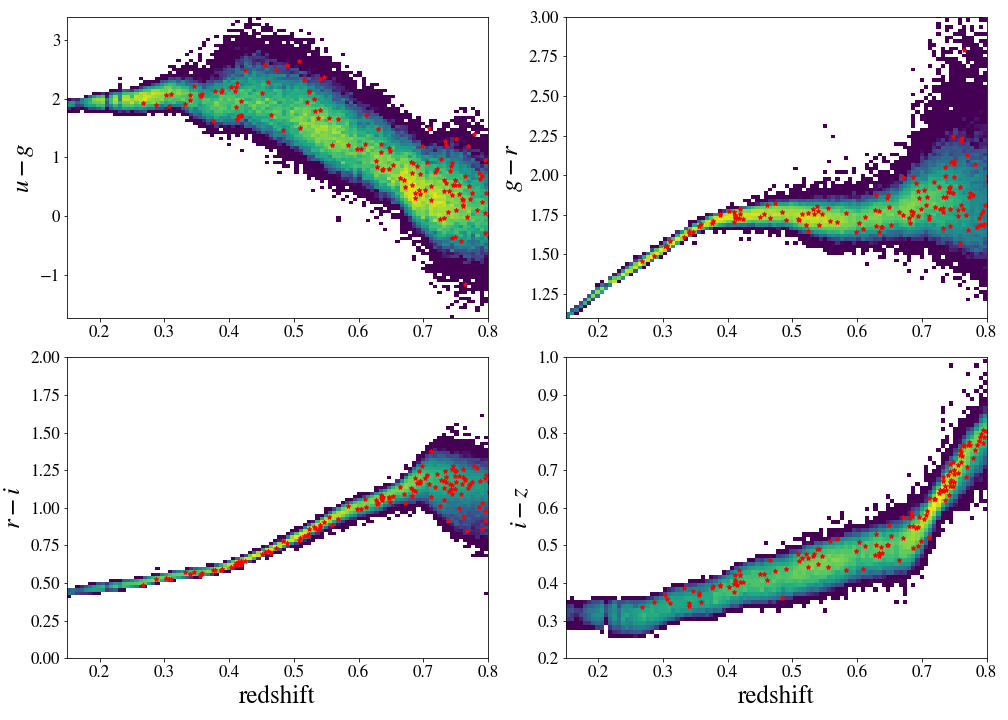
\includegraphics[width=\textwidth]{figures_tmp/cosmos_color.png}
\caption{Distribution of the selected luminous red-sequence galaxies in colour  space as a function of redshift (colour map). The COSMOS-G10 galaxies are shown as red stars. In each panel, the colour  scale denotes the number density of luminous red galaxies in the colour -redshift space, with yellow corresponding to higher number densities and blue corresponding to lower number densities.} 
\label{fig:cosmos_color}
\end{figure*}

\begin{figure}
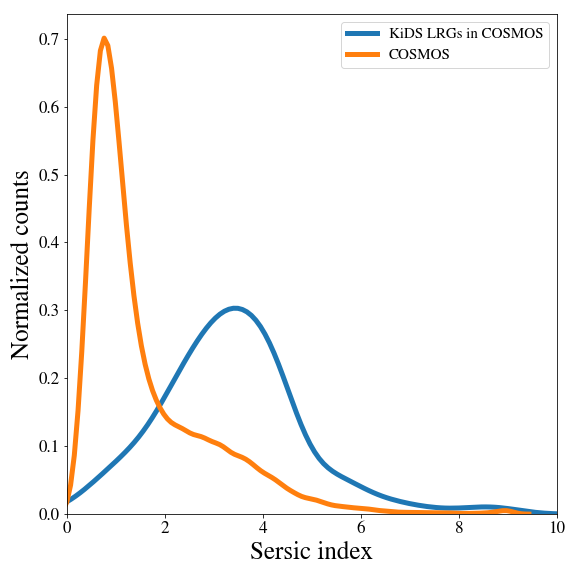
\includegraphics[width=\columnwidth]{figures_tmp/cosmos_sersic.png}
\caption{Distribution of S\'{e}rsic indices of luminous red-sequence galaxies in COSMOS (blue) versus the that of all galaxies in COSMOS (orange). The selected red-sequence galaxies tend to have larger values of S\'{e}rsic indices compared to all galaxies in the COSMOS region.}
\label{fig:cosmos_sersic}
\end{figure}

\begin{figure*}
\begin{tabular}{cc}
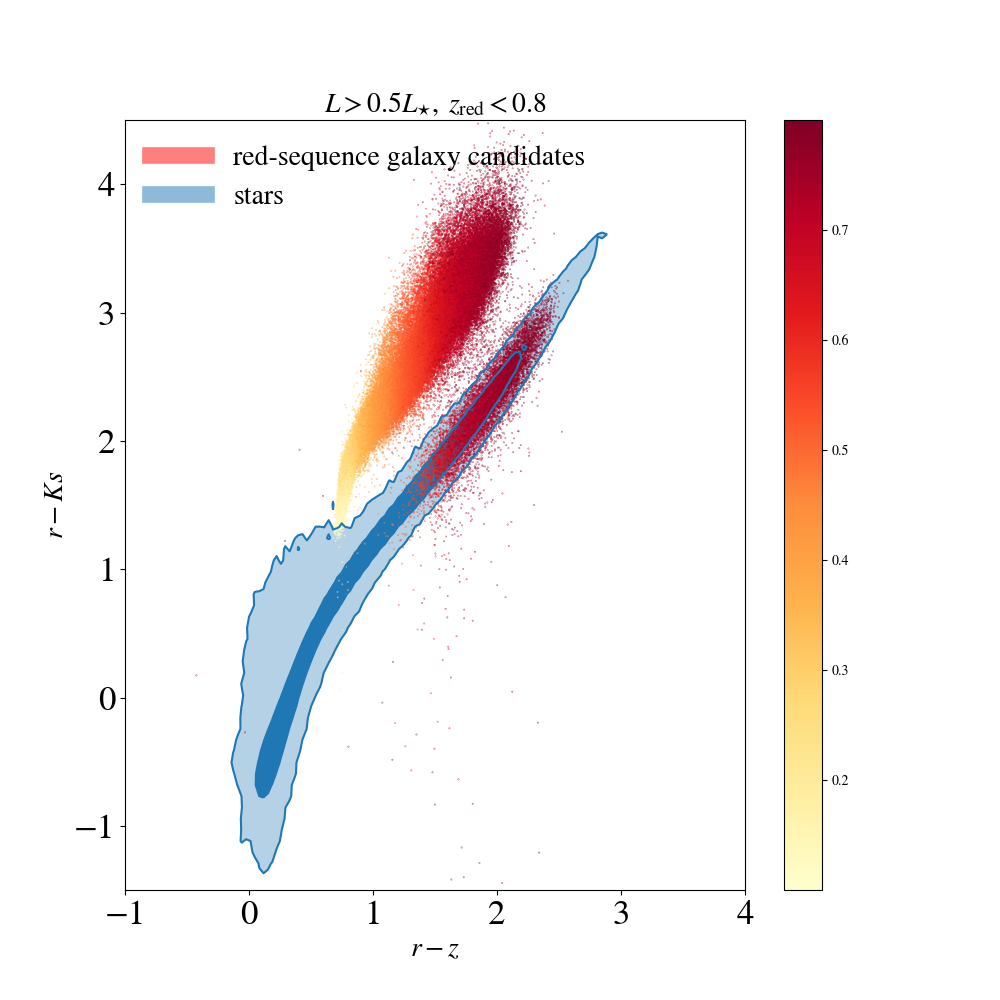
\includegraphics[width=0.5\textwidth]{figures_tmp/red_vs_star_dense.png}
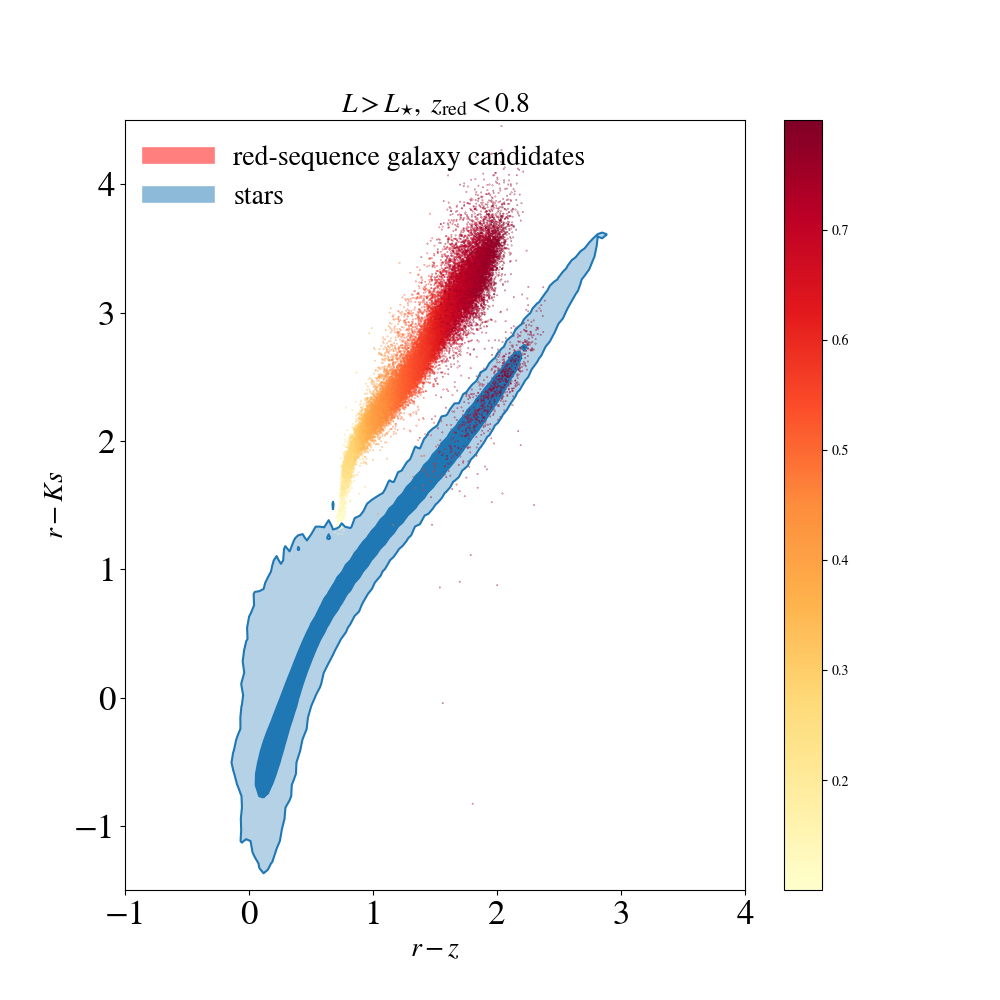
\includegraphics[width=0.5\textwidth]{figures_tmp/red_vs_star_lum.png}
\end{tabular}
\caption{ Demonstration of the use of optical+NIR colours for the identification of likely stellar objects amongst the red-sequence galaxy candidates. 
In each panel, the points colour-coded with redshift show the red-sequence candidates in the $(r-K_{\rm s}) \times (r-z)$ space, while the blue contours show the 68\% and 95\% confidence regions of the distribution of high confidence stars. Left Panel: At high redshifts ($z_{\rm red}>0.6$), the considerable overlap between the distribution of red-sequence candidates in the dense sample ($L>0.5L_{\star}$) and that of the high confidence stars becomes clear. Right Panel: In the case of the red-sequence candidates in the luminous sample ($L>L_{\star}$), the overlap between the two distributions is less apparent.} 
\label{fig:star_galaxy_I}
\end{figure*}


\begin{figure*}
\begin{tabular}{cc}
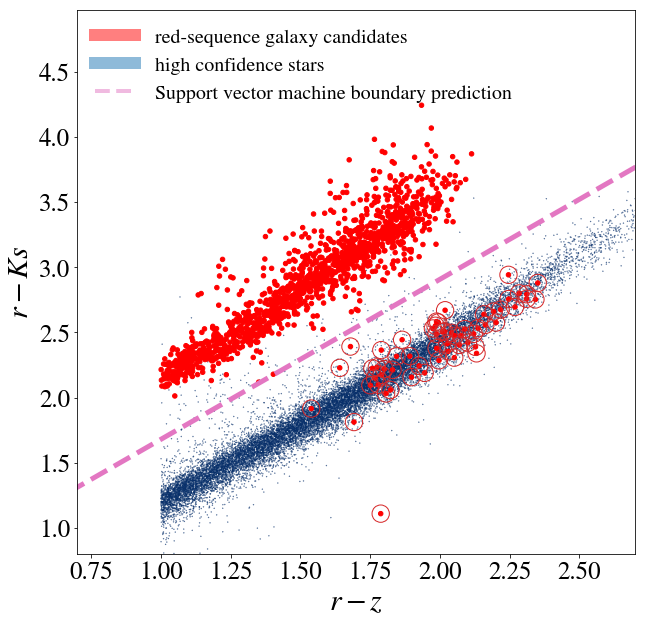
\includegraphics[width=0.5\textwidth]{figures_tmp/stars_SVM_lum.png}
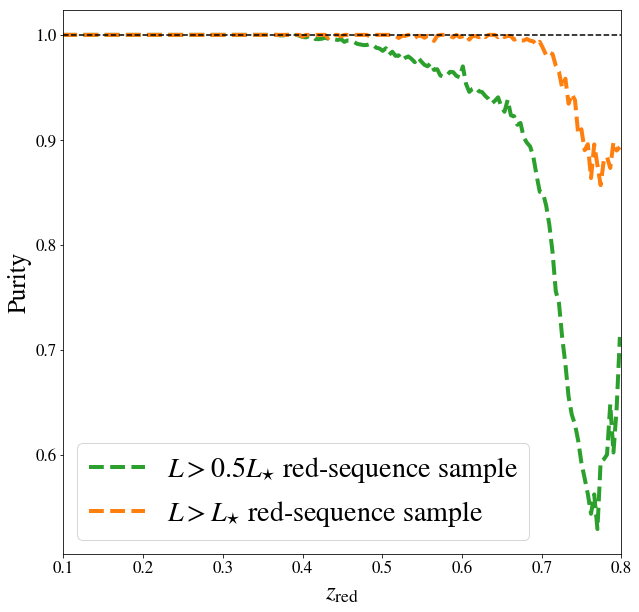
\includegraphics[width=0.5\textwidth]{figures_tmp/lrg_purity.png}
\end{tabular}
\caption{ Left Panel: At redshifts above $z_{\rm red}>0.4$ red-sequence galaxies (shown in red) and high confidence stars (shown in blue) reside in separated regions of the two-dimensional $(r-K_{\rm s}) \times (r-z)$ colours. Shown in pink dashed line is the predicted decision boundary between the two classes. The red-sequence candidates falling below the predicted boundary are marked by open circle. These objects are flagged as likely stellar objects in the final catalogue, and thus removed from our large-scale structure analysis. Right Panel: Purity fraction of the dense  (green dashed line) and the luminous (orange dashed line) samples as a function of redshift.}
\label{fig:star_galaxy_II} 
\end{figure*}

\begin{figure}
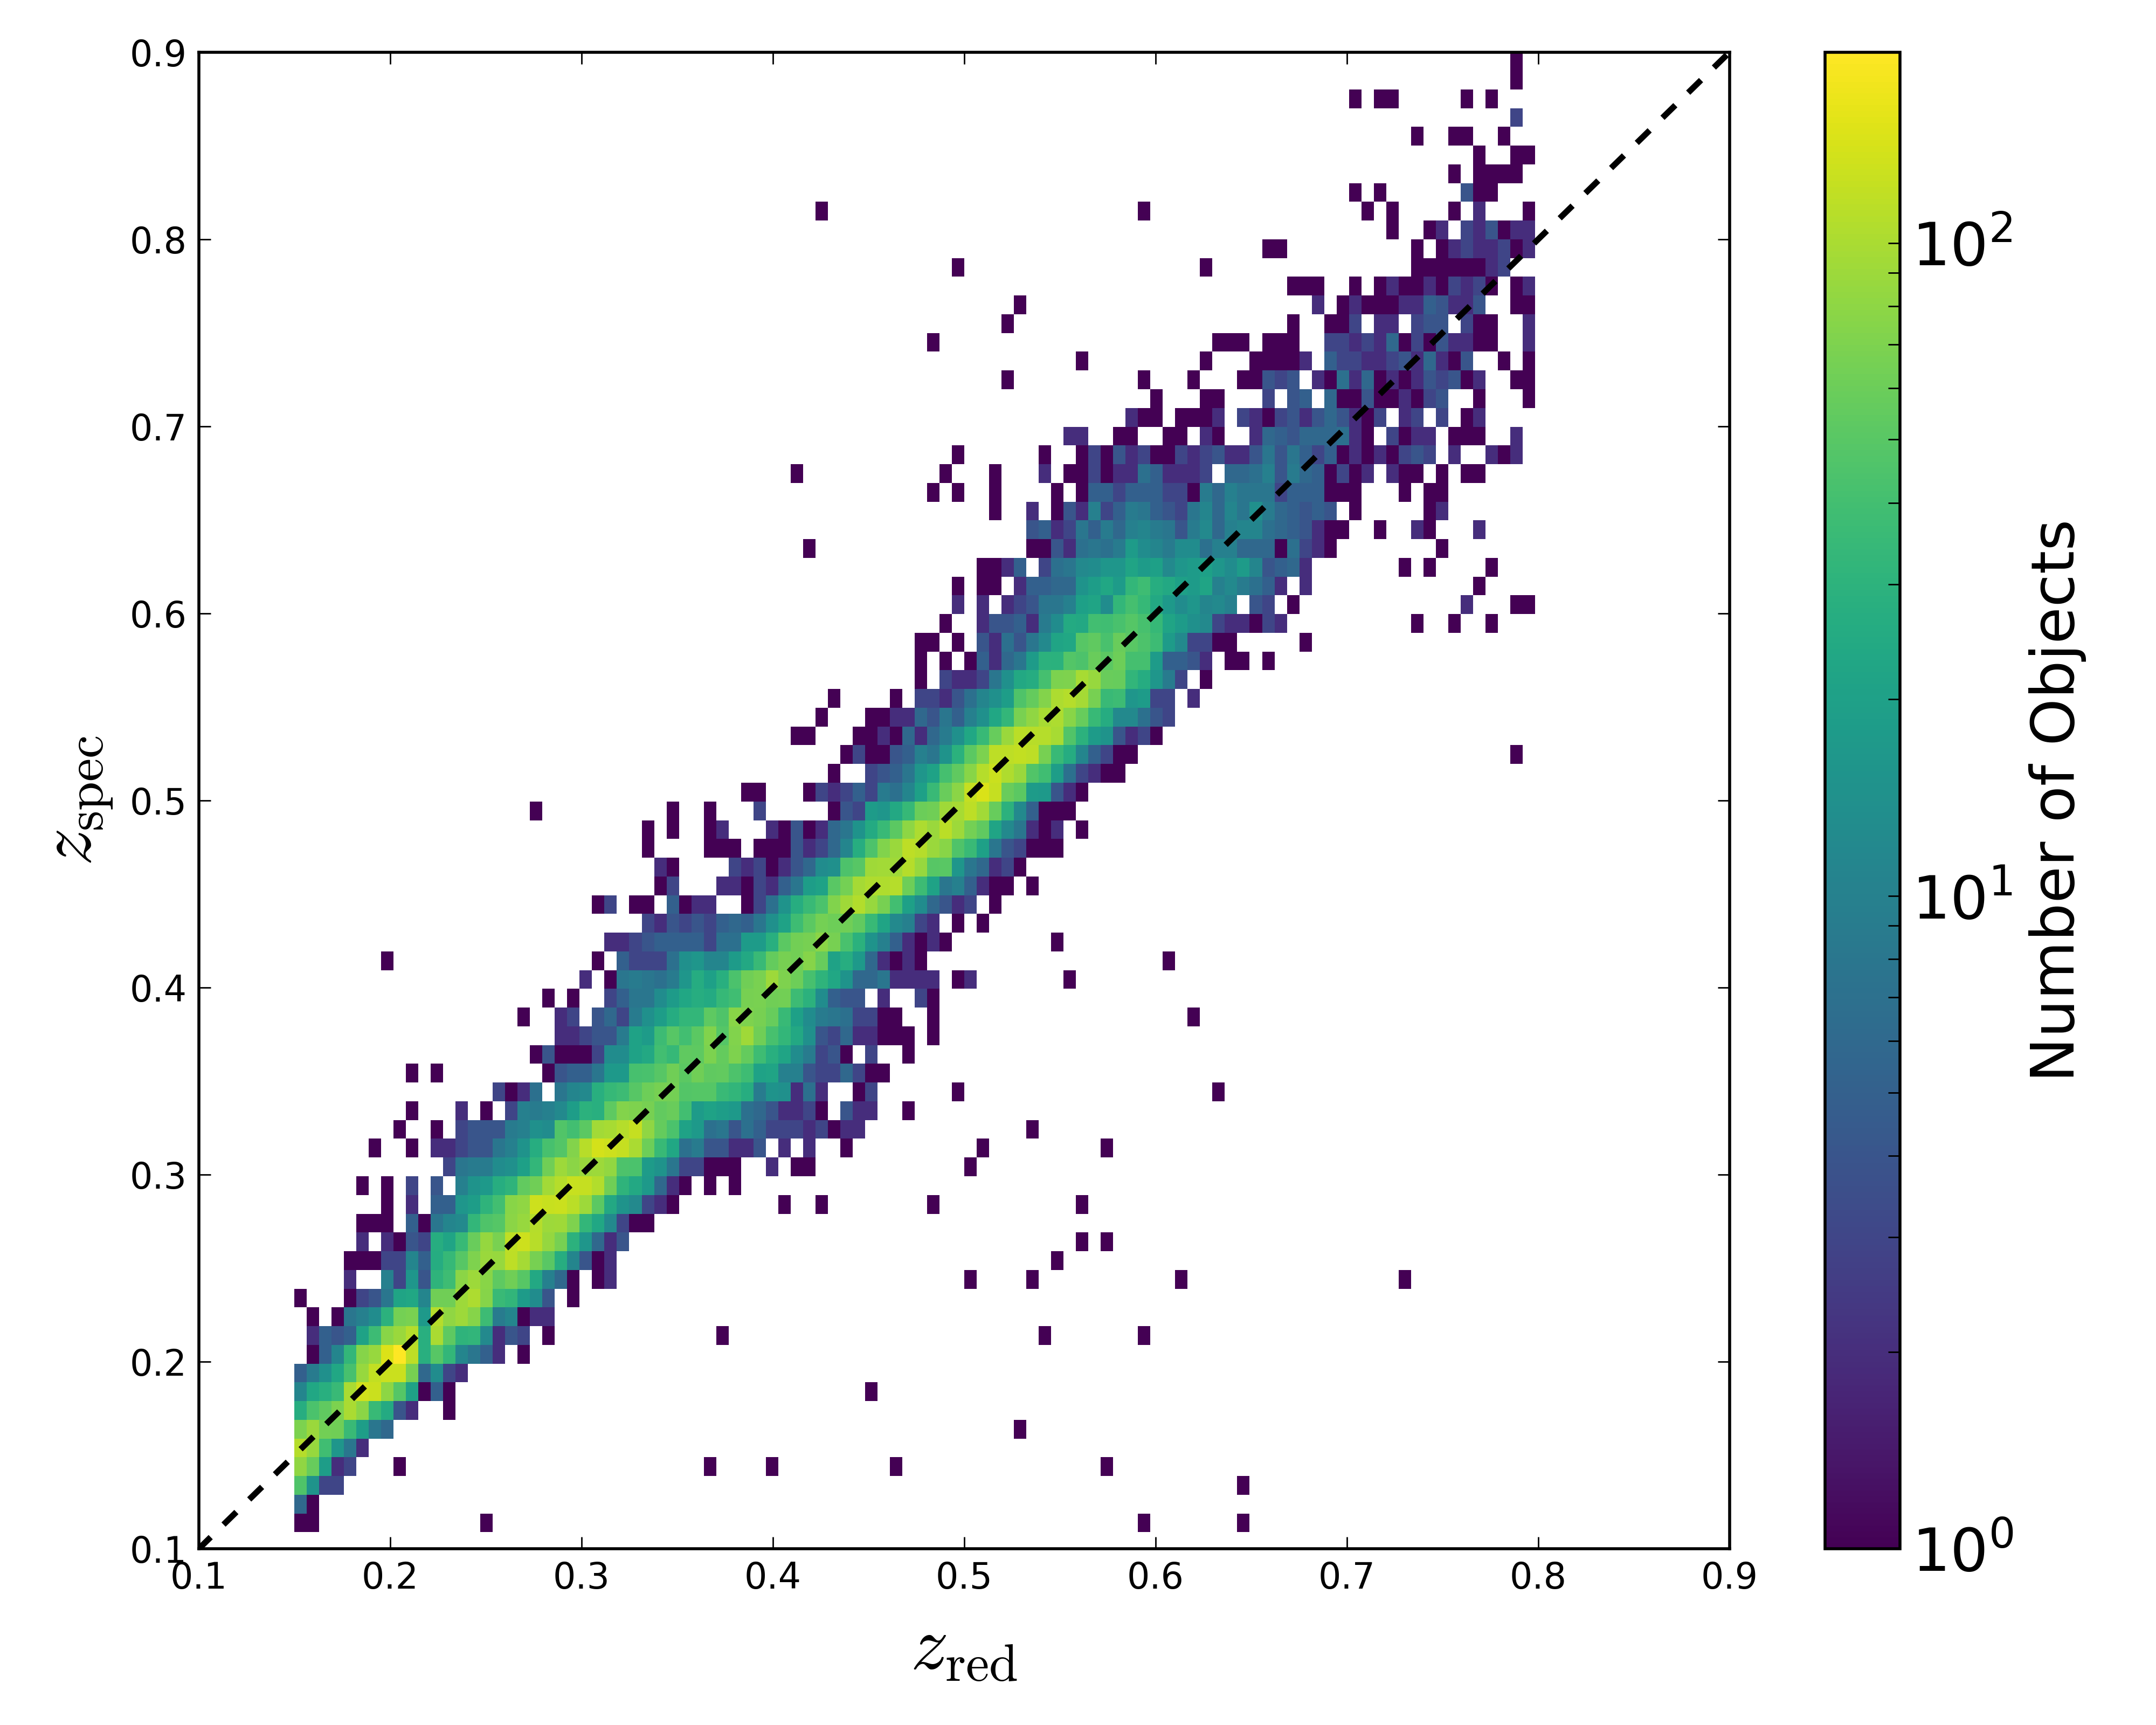
\includegraphics[width=\columnwidth]{figures_tmp/zphotscatter_new.png}
\caption{Comparison between the estimated red-sequence redshifts and spectroscopic redshifts for galaxies with spectroscopy.} 
\label{fig:zphotscatter}
\end{figure}


%\begin{figure}
%    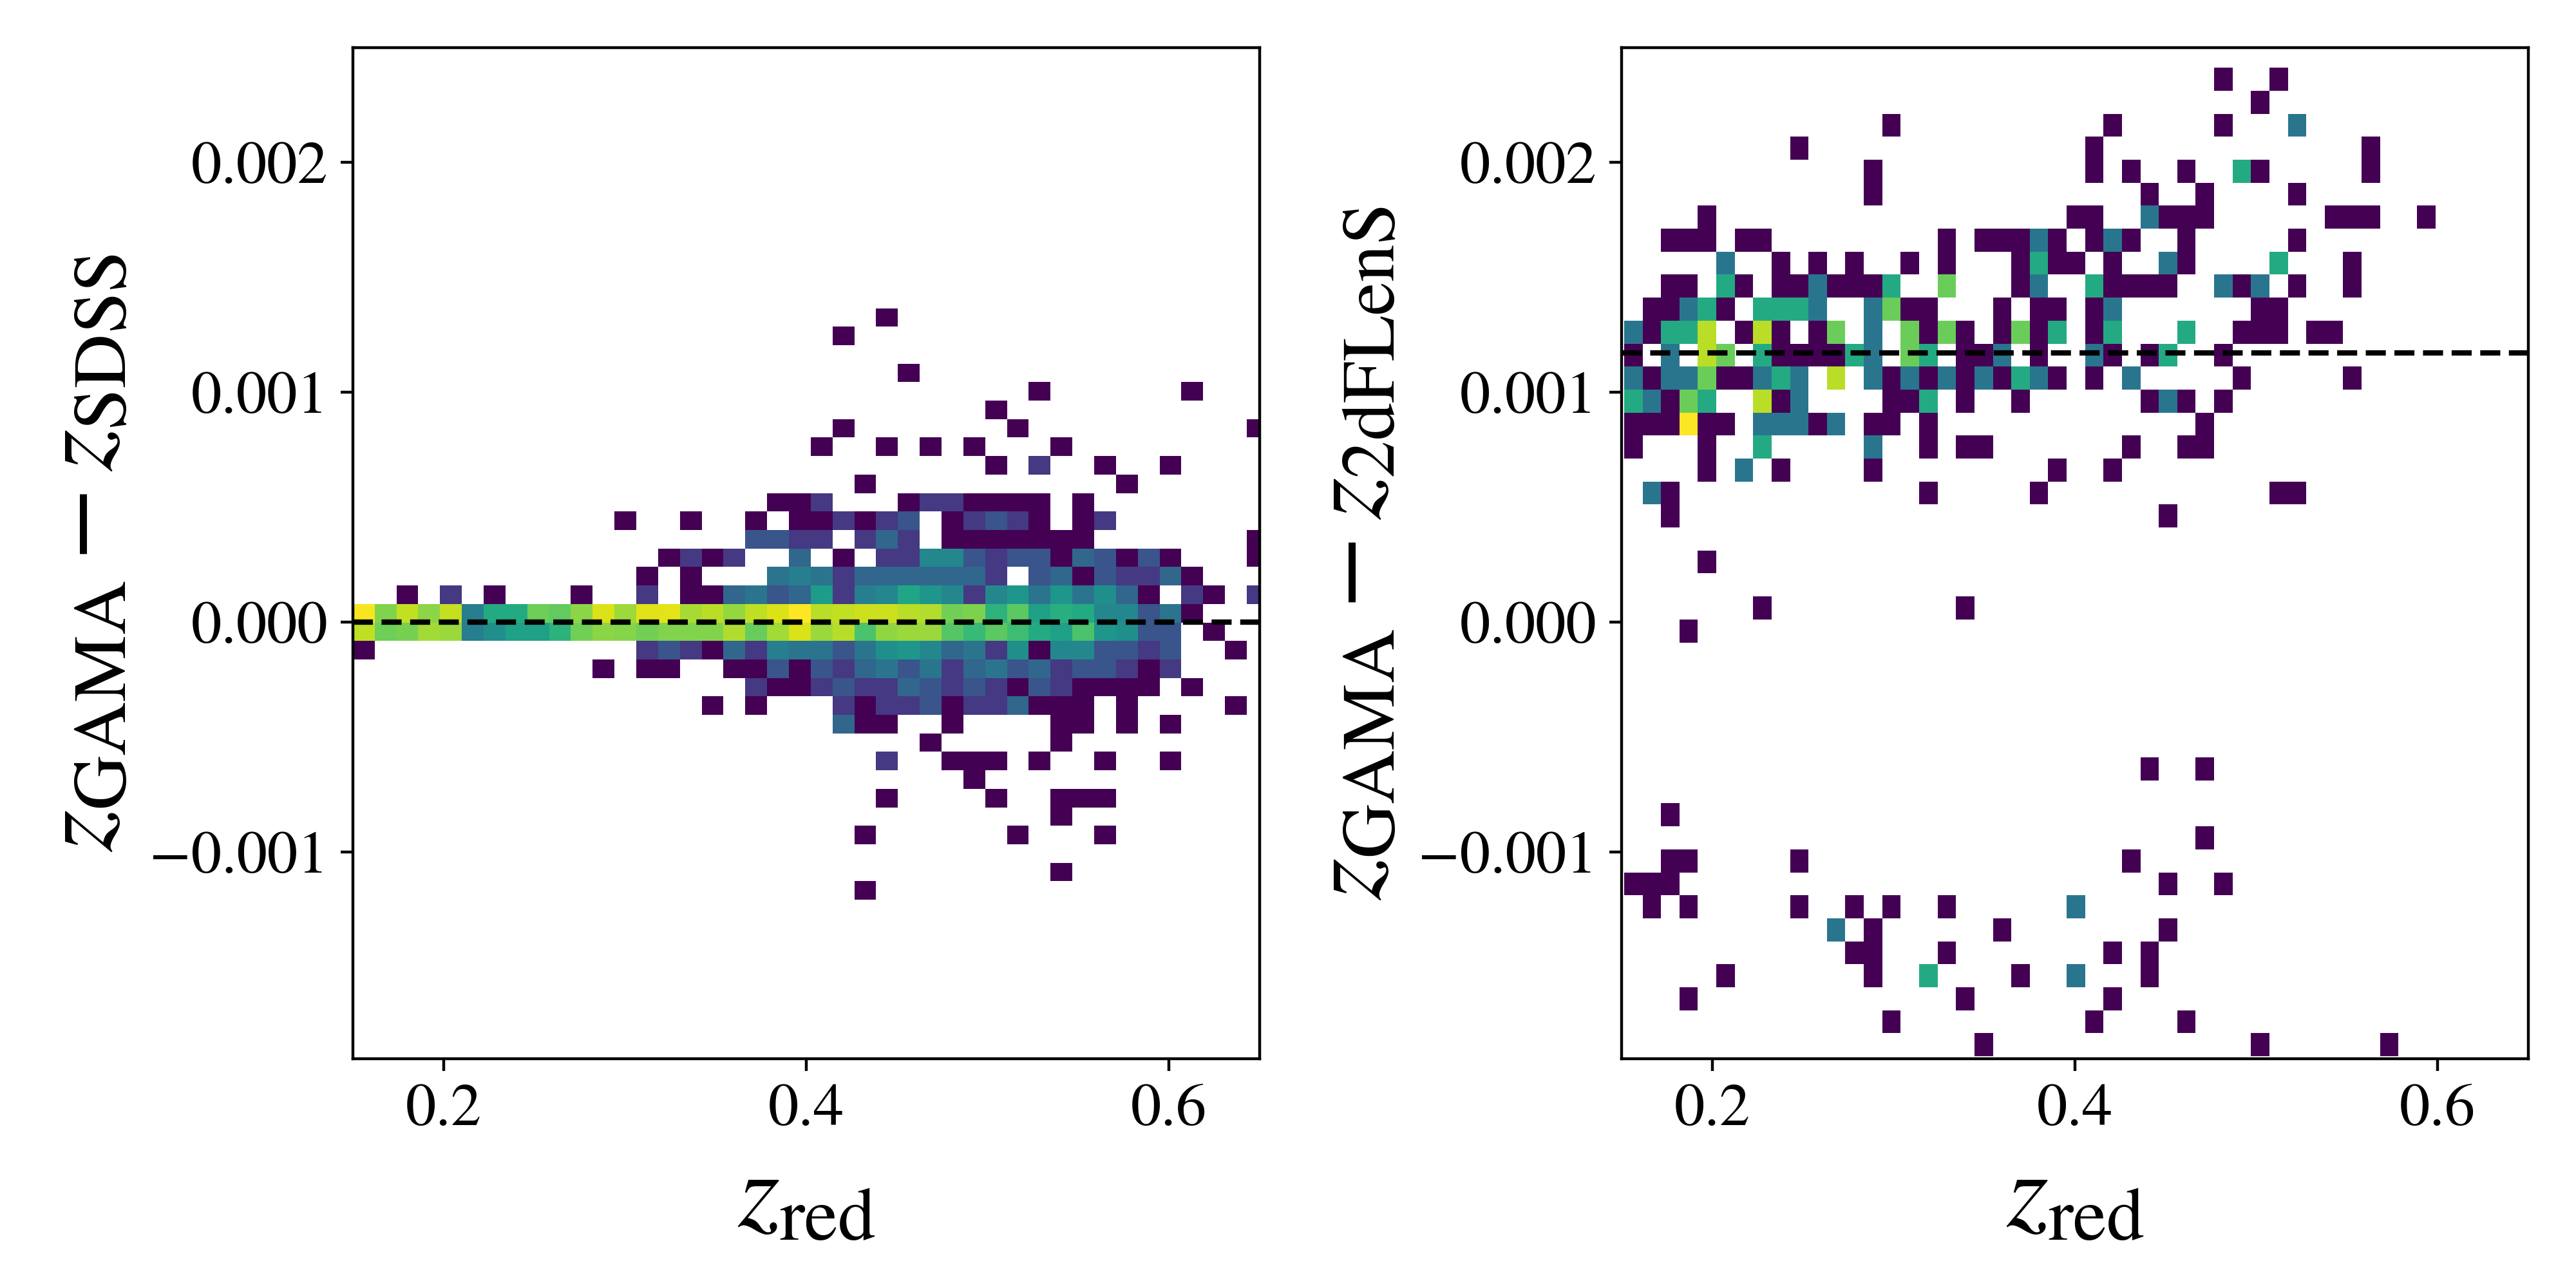
\includegraphics[width = \columnwidth]{figures_tmp/diff_spec.png}
%    \caption{Test of consistency between the spectroscopic data sets for the selected red-sequence galaxies targeted by multiple spectroscopic surveys. Left (right) Panel: Joint distribution of $z_{\rm red}$ the offset between $z_{\rm GAMA}$ and $z_{\rm SDSS}$ ($z_{\rm 2dFLenS}$). In each panel, the median of the difference between the spectroscopic redshifts.}
%    \label{fig:student-t}
%\end{figure}


\begin{figure}
    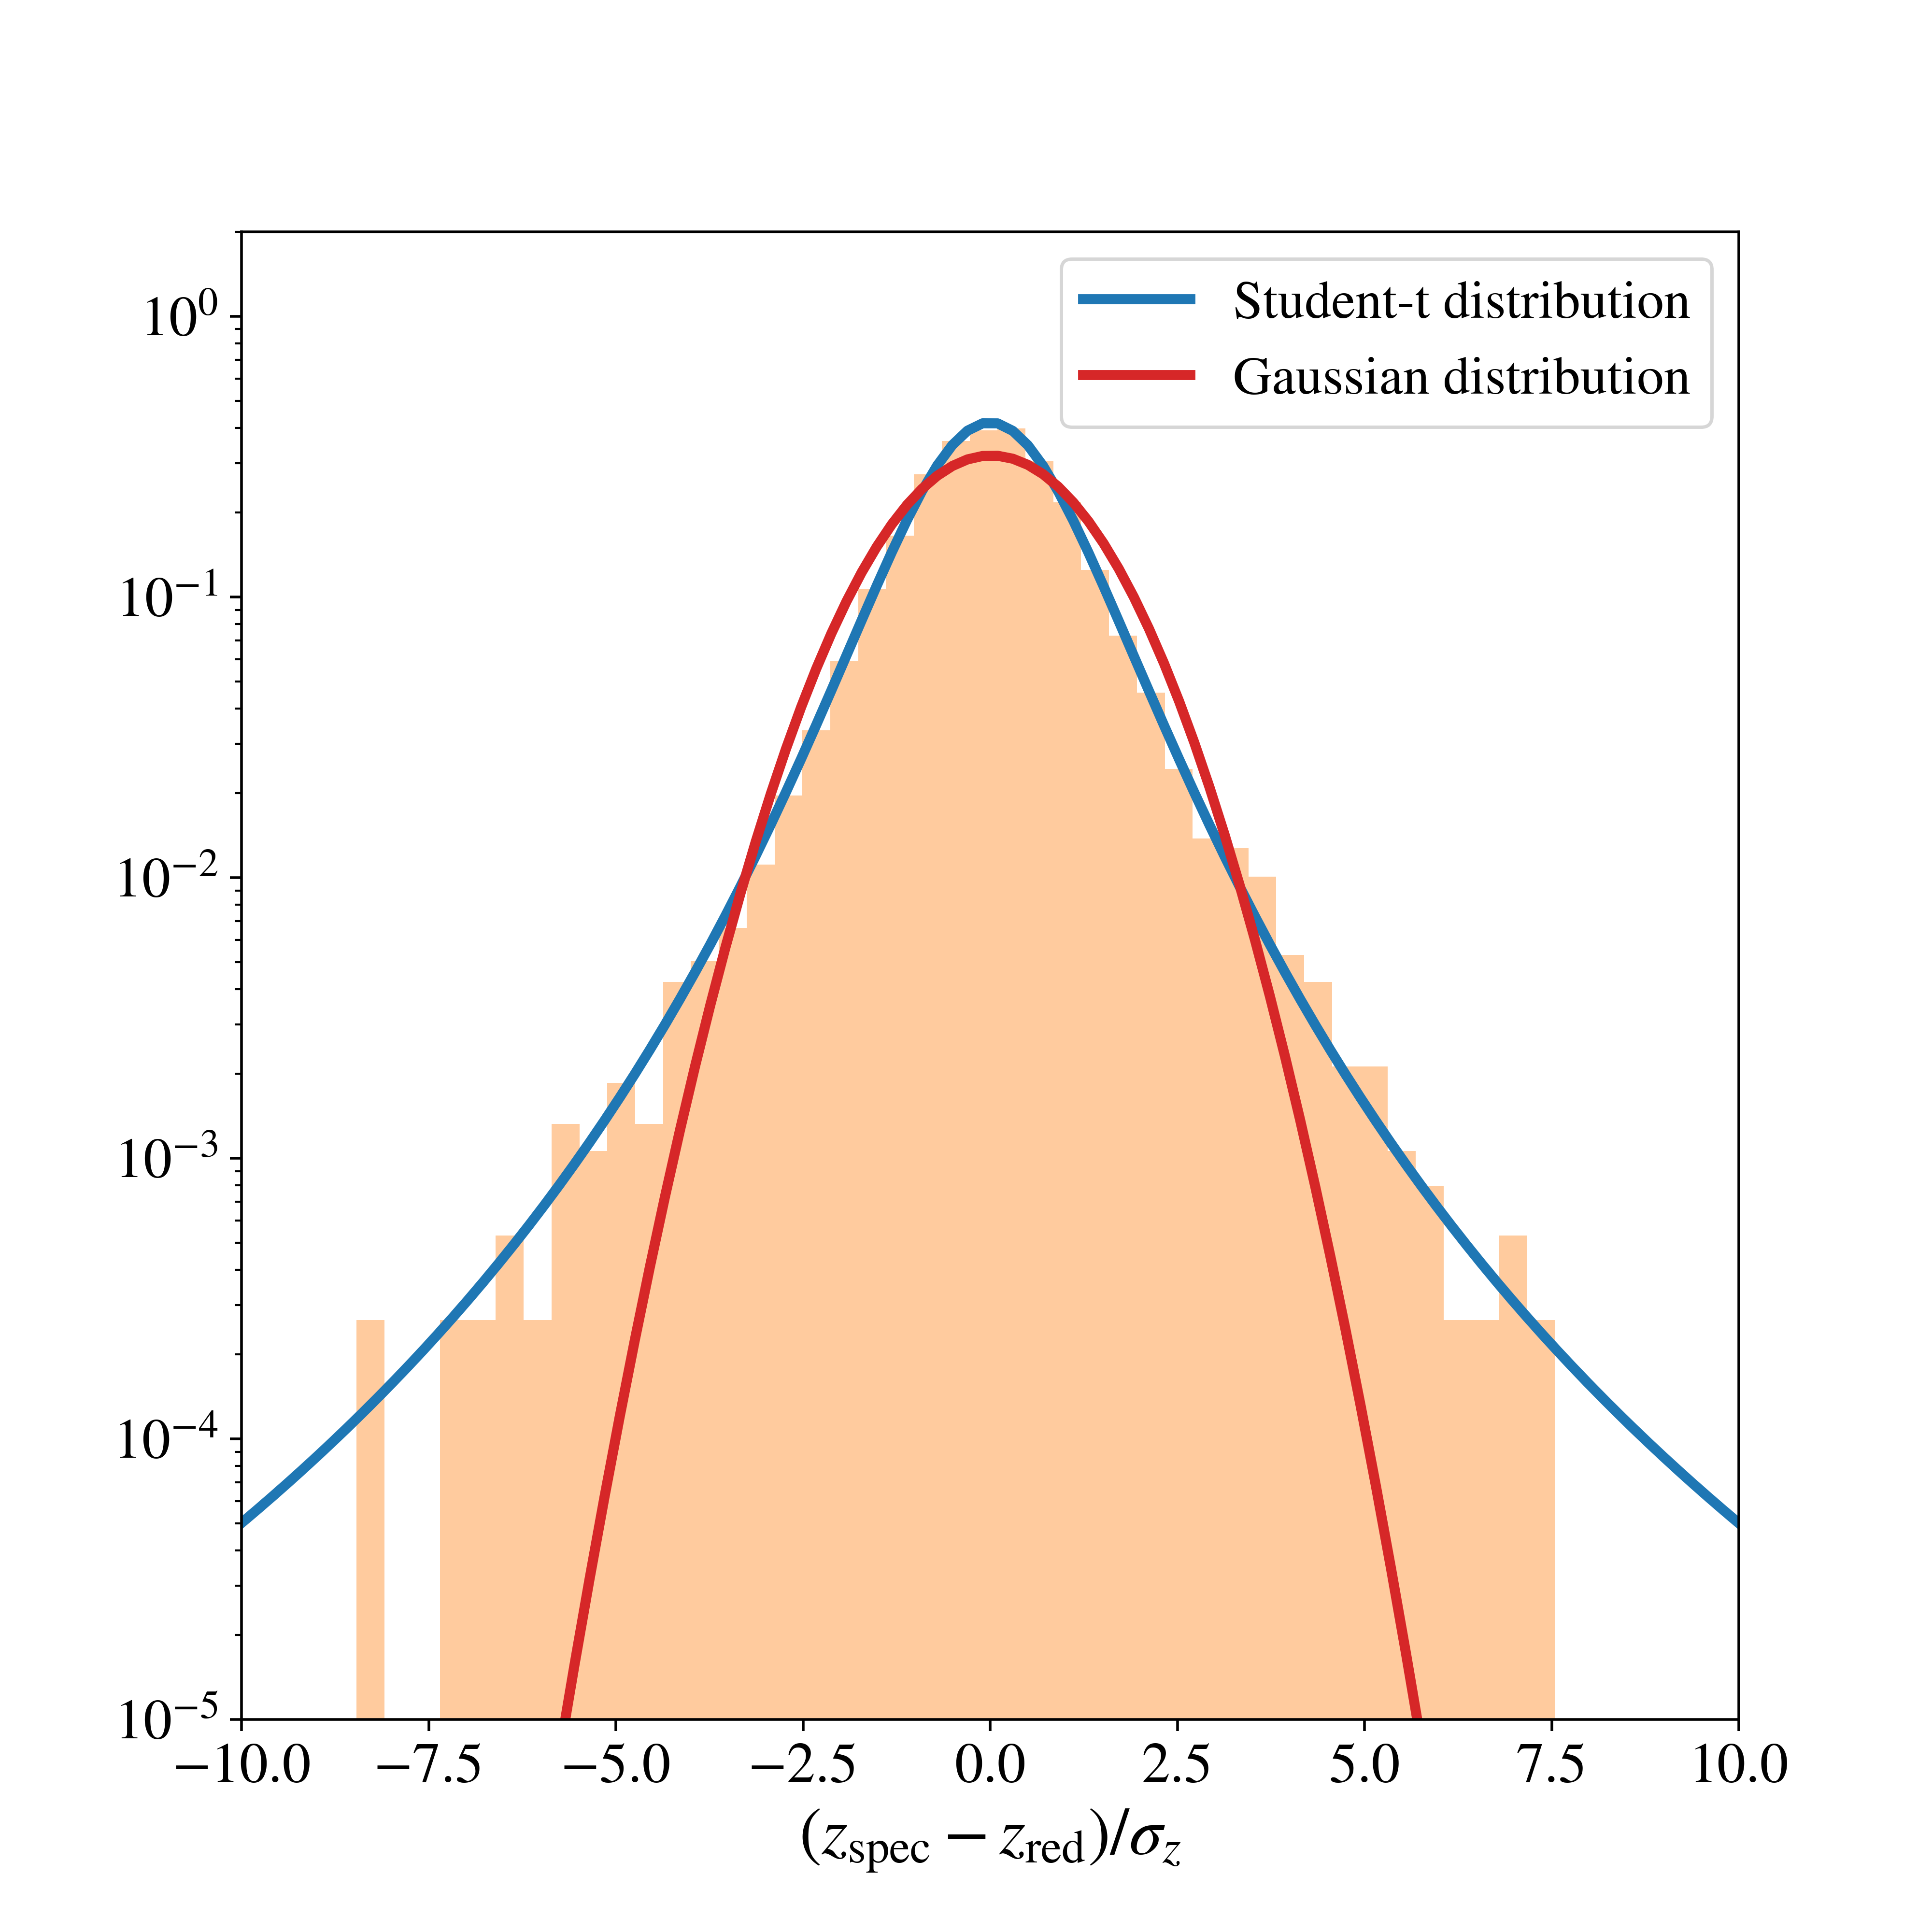
\includegraphics[width = \columnwidth]{figures_tmp/student_t.png}
    \caption{The distribution of the quantity $(z_{\rm spec} - z_{\rm red})/\sigma_z$ is shown in orange. Shown in blue (red) is the best-fit Student-t (Gaussian) distribution. A Student-t distribution provides a better description of the long-tails of the redshift distributions of individual galaxies.}
    \label{fig:student-t}
\end{figure}


\begin{figure}
    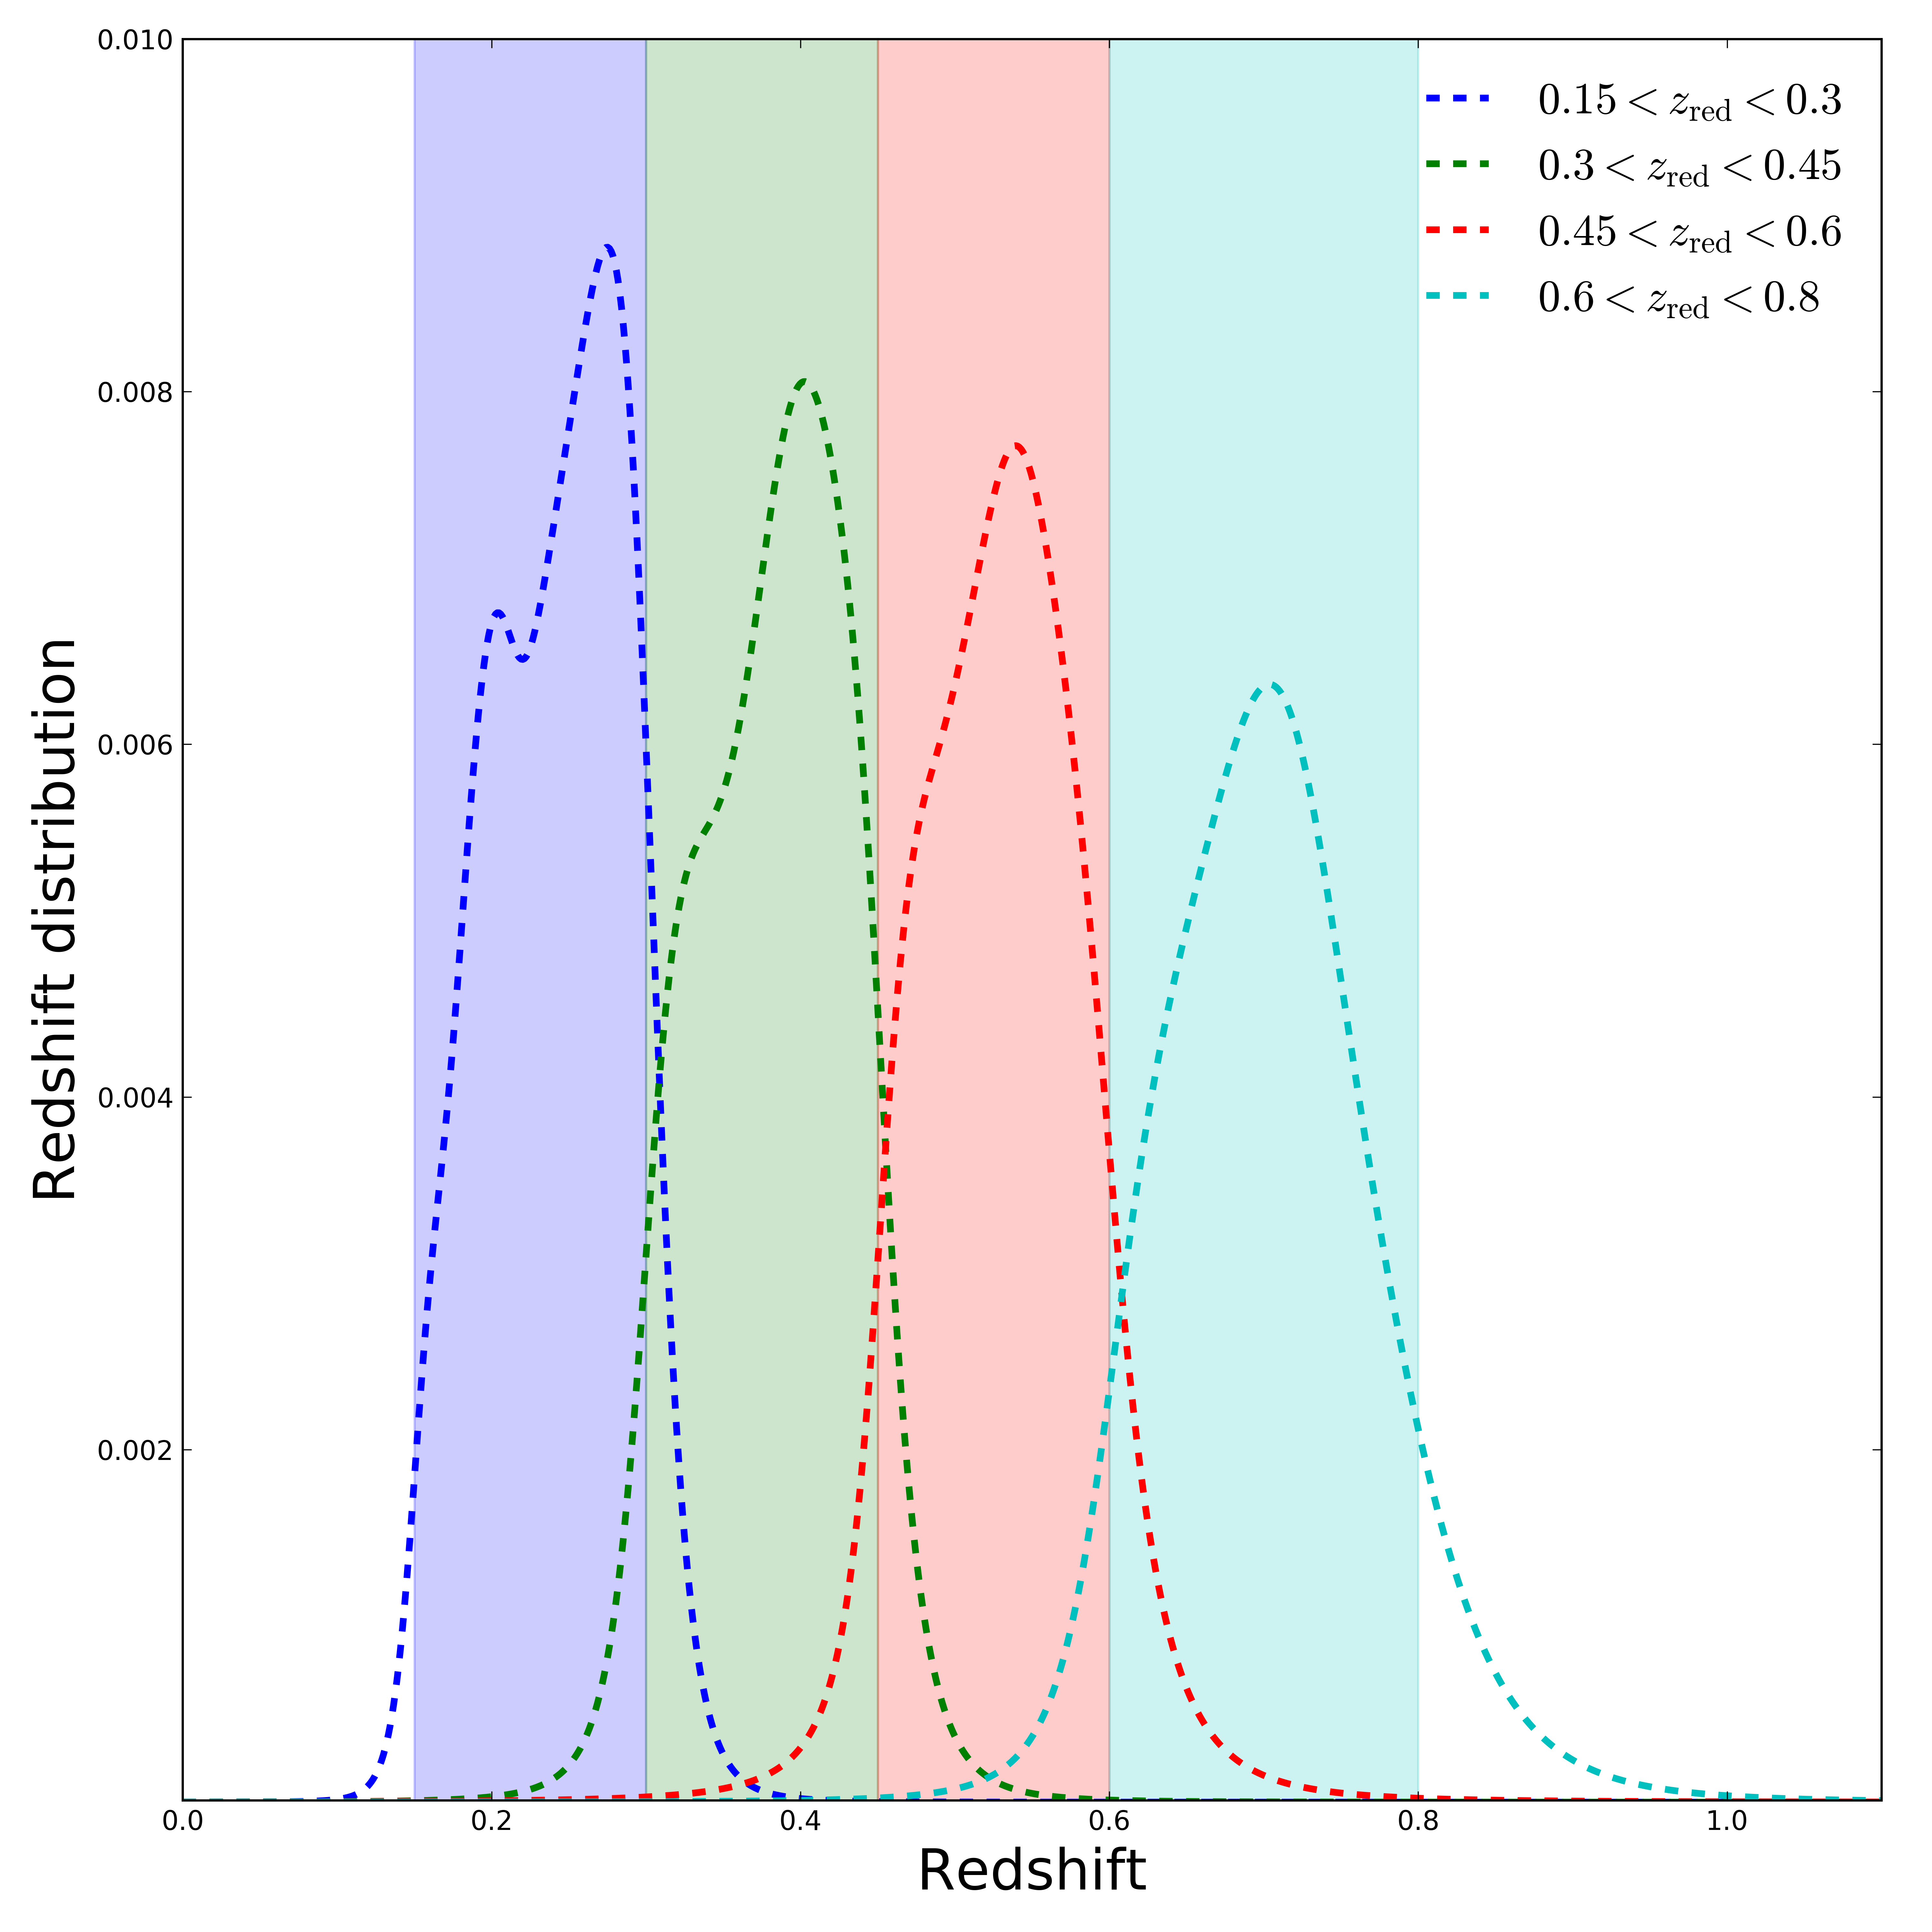
\includegraphics[width = \columnwidth]{figures_tmp/nzs.png}
    \caption{The redshift distributions of the four redshift bins designed for studying the large-scale structure.The shaded regions mark the redshift boundaries used for defining the redshift bins.}
    \label{fig:nzs}
\end{figure}

%'gama', 0.15, -0.003315041887105681)
%('sdss', 0.15, 0.0037563046212067785)
%('df', 0.15, -0.0023803744911023695)
%('cosmos', 0.15, 0.00173914528107969)
%('gama', 0.3, -0.0009886939301030784)
%('sdss', 0.3, -0.0010892662824363753)
%('df', 0.3, -0.0001029462380064855)
%('cosmos', 0.3, 0.003765066560434964)
%('gama', 0.45, 0.004774418194529906)
%('sdss', 0.45, -0.004102710197294344)
%('df', 0.45, -0.002175855388768679)
%('cosmos', 0.45, 0.0014348330273191298)
%('gama', 0.6, 0.007963050133684446)
%('sdss', 0.6, 0.0016848169637070582)
%('df', 0.6, 0.0038241223404244648)
%('cosmos', 0.6, -0.0157947535517734)





\section{Sample selection}\label{sec:selection}

\subsection{Red-sequence model}

Several aspects of the selection procedure in this work are similar to what has been outlined  in~\citet{vakili2019}. In what follows we describe the main distinctions. Previously, we only utilized the KiDS optical photometry for our red-sequence model. In this work, we also include the VIKING $Z$ band in the red-sequence template.
The added advantage of the $Z$ band is the additional constraining power on the redshifts of the red-sequence galaxies at higher redshifts ($z>0.7$)\footnote{In principle, one can also include the $YJHK_{\rm s}$ bandpasses of VIKING in the red-sequence model. However, we decided to exclude those bands in the modelling as they would increase the computational cost of the following steps: Selection of a set of seed galaxies (with spectroscopic redshifts) for estimating the parameters of the red-sequence template, and eventually computing the conditional probability of colours conditioned on the redshift and magnitudes for all the objects in the survey. \mb{[I believe this footnote should be within main text]}}.
%This allows the complexity of our model to be similar to that of~\citet{rozo2016} with the exception of the presence of the $u$ band.

%\mb{[the same was already said in the data section - I suggest removing this paragraph]}
%As we discussed in Section~\ref{sec:data}, we use the apparent $\mathtt{AUTO}$ magnitude in the $r$-band which is provided in KiDS DR4 as $\mathtt{MAG\_AUTO}$\footnote{The $\mathtt{AUTO}$ magnitudes are not provided for the rest of the KiDS-VIKING bands in KiDS DR4.} As discussed in Section~\ref{sec:data}, we use the GAaP $\{u-g,g-r,r-i,i-Z\}$ colours, which provide a more precise estimate of the colours of objects (\citealt{kuijken2019}). 

Our data-driven model of the colours of the red-sequence galaxies is fully characterized with the probability of the colours of red galaxies conditioned on their apparent magnitudes and redshifts: $p(\boldsymbol{c}|m,z)$. After evaluating this probability distribution for every object in the survey, we proceed in a similar fashion as described in detail in \citet{rozo2016, vakili2019}. We construct two luminosity-threshold sample with the luminosity ratio is defined as
\begin{equation}
    \log_{10}\Big(\frac{L}{L_{\star}}\Big) = -0.4\big(m_{r} - m_{r}^{*}(z)\big), 
\end{equation}
in which the characteristic magnitude $m_{r}^{*}(z)$ is evaluated using the EZGAL (\citealt{ezgal_paper}) implementation of the \citet{bc03} stellar population model. The two luminosity-threshold samples are called the dense sample with $L>0.5 L_{\star}$ and the luminous sample with $L>L_{\star}$. Additionally, we run our selection algorithm on the galaxies in the GAMA-G10 catalogue which are not present in KiDS DR4.%\mb{[see my comment above regarding COSMOS not being within DR4]}.

For the luminous sample, we show the evolution of the GAaP colours with respect to the estimated red-sequence redshifts in Figure~\ref{fig:cosmos_color}. The red points show the red-sequence galaxies with $L>L_{\star}$ in the GAMA-G10 COSMOS field. These galaxies are selected in a consistent manner and hence, they follow the redshift-dependent colour distribution of the luminous red-sequence sample in KiDS DR4. 

Figure~\ref{fig:cosmos_color} offers an intuitive picture of how different colours contribute to determination of the redshifts of red galaxies\footnote{Note that in this intuitive description we have neglected the magnitude dependence of the red-sequence template which plays an additional constraining role in determining the redshifts.}. At low redshifts, the $g-r$ colour rises sharply with increasing redshift. As the 4000 \AA break moves between the broadband filters, the $g-r$ colour reaches a relative plateau while the $r-i$ colour starts a rapid increase. At high redshifts however, it is the $i-Z$ colour that shows a higher sensitivity to the redshift of red galaxies. The $u-g$ colour shows a slow and noisy decline considering that red galaxies become fainter in the $u$ filter at higher redshifts. 

%\begin{figure}
%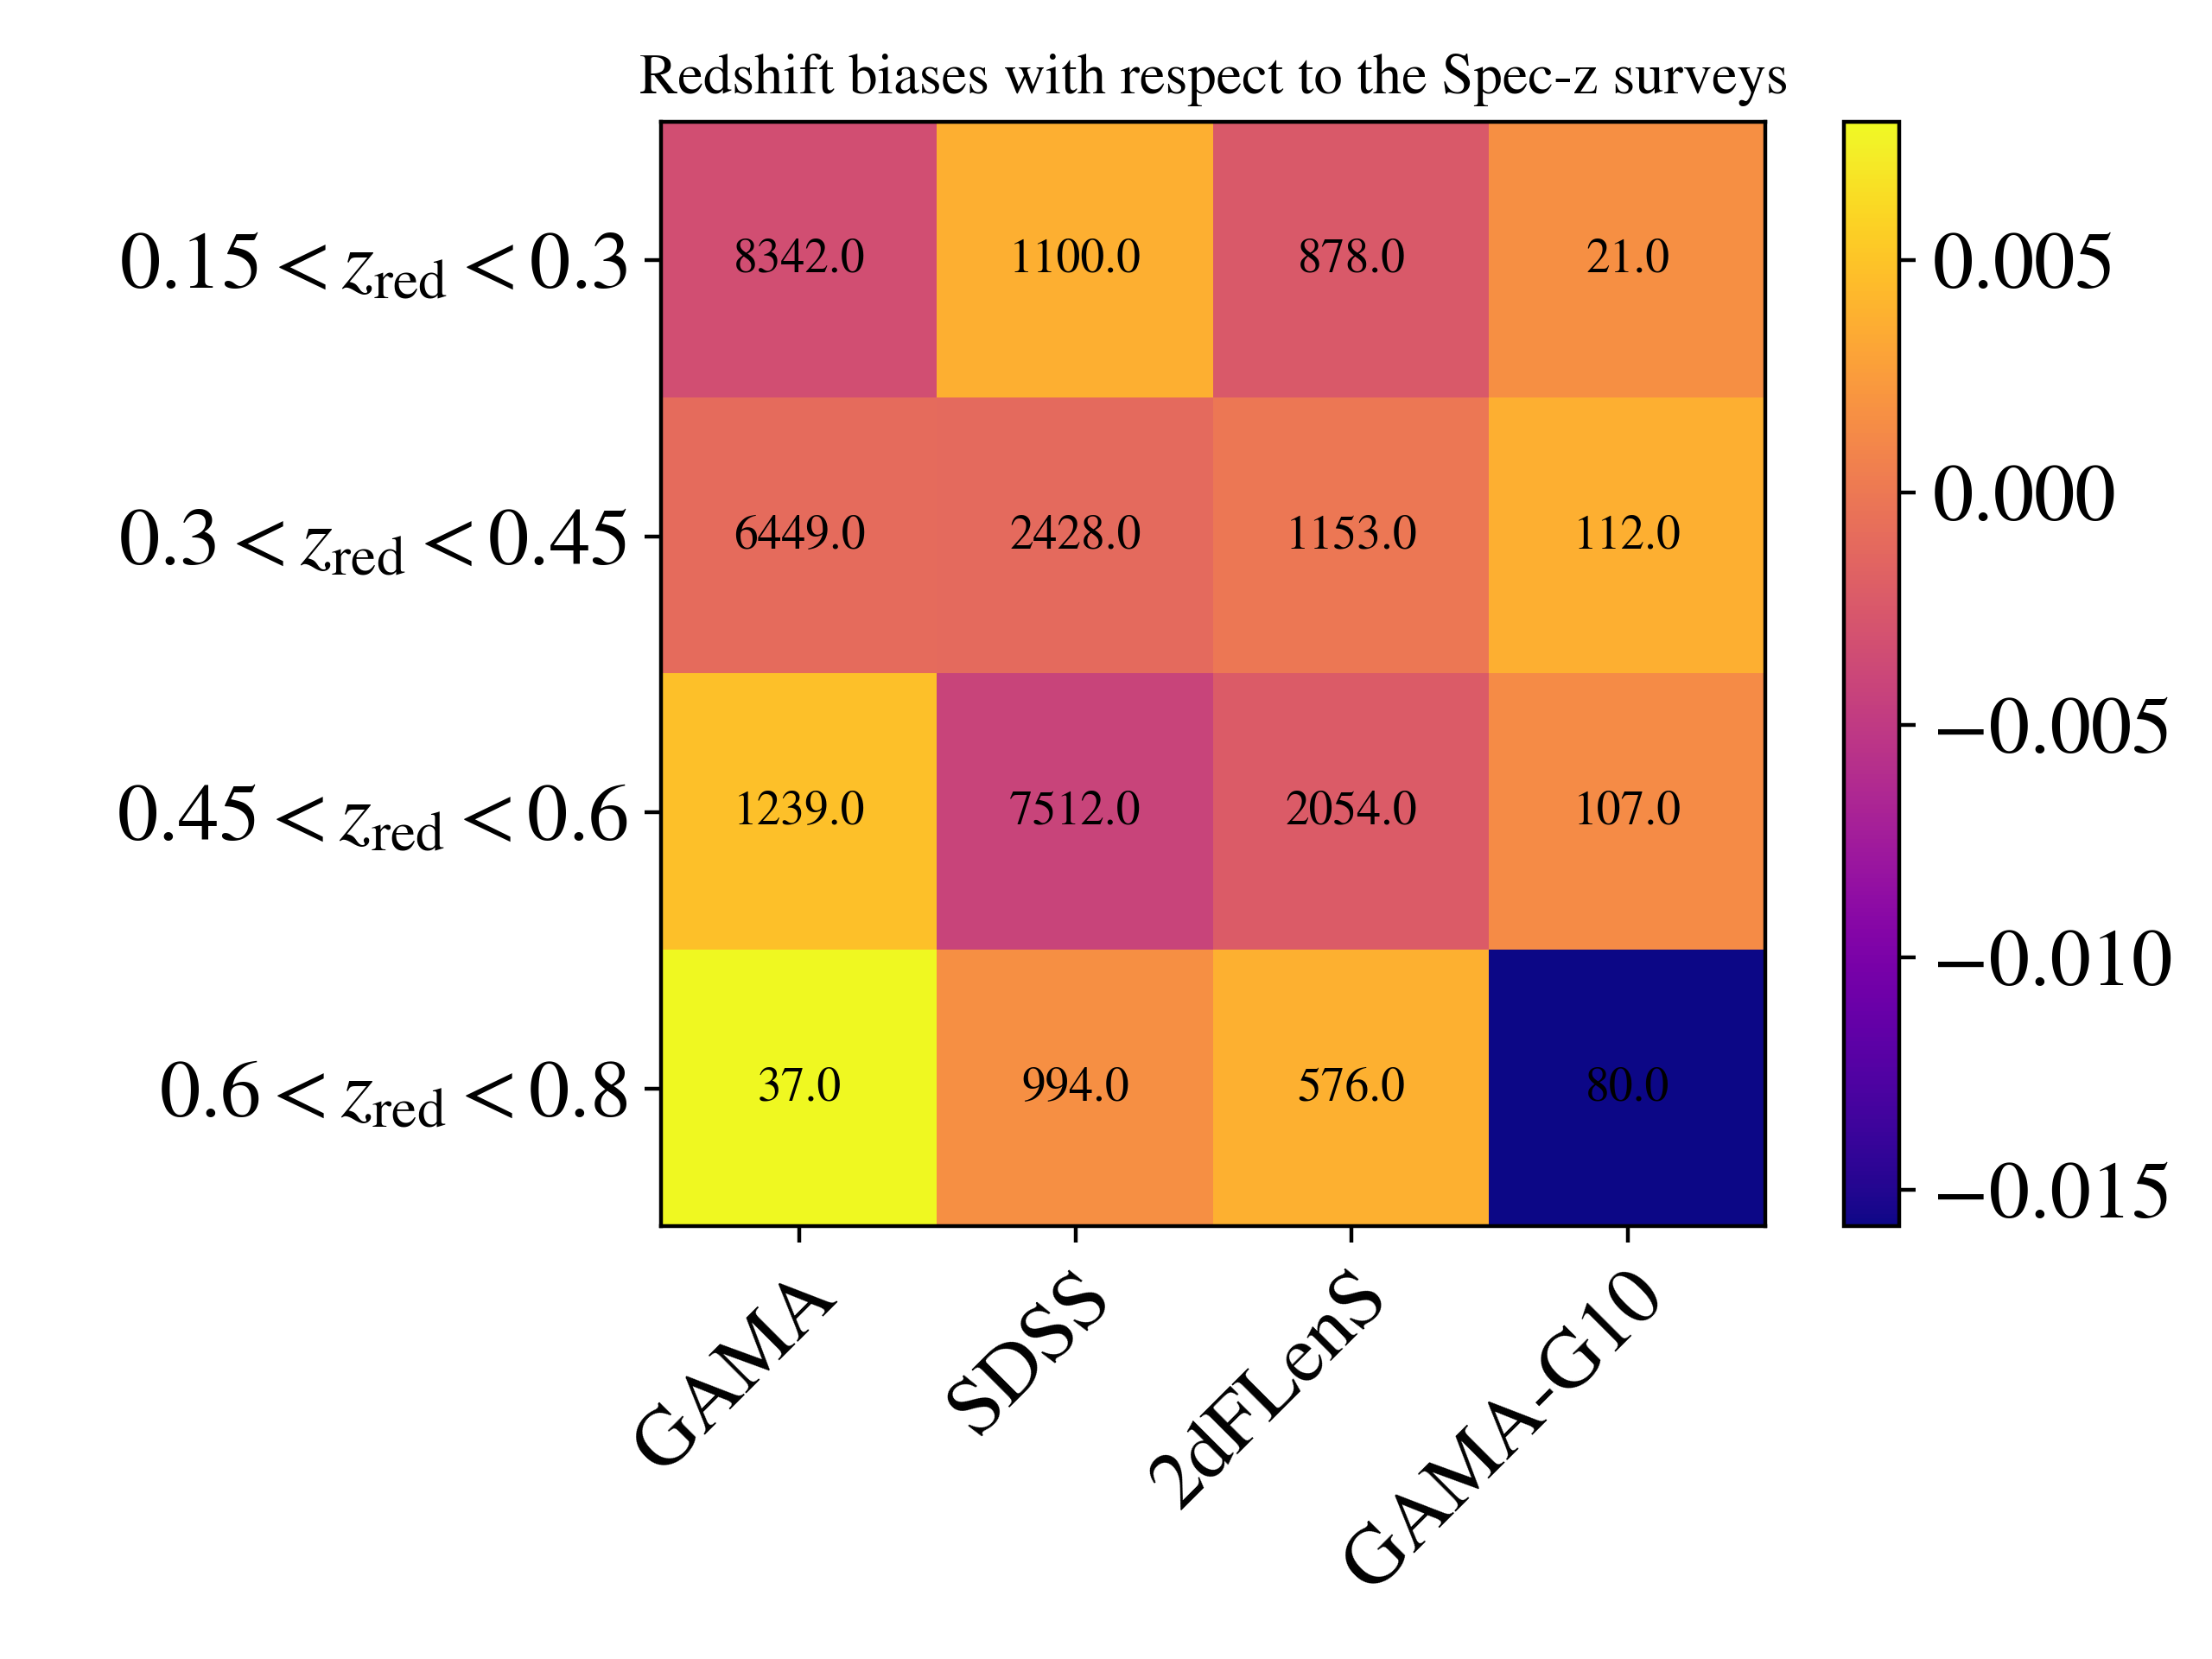
\includegraphics[width=\columnwidth]{figures_tmp/sys/photoz_bias.png}
%\caption{\label{fig:photoz_bias}Comparison between the estimated red-sequence %redshifts and spectroscopic redshifts of galaxies with spectroscopy.} 
%\end{figure}



We are also interested in the morphological properties of the selected sample, i.e. whether the selected galaxies tend to have elliptical morphology. We match the red-sequence galaxies in the GAMA-G10 field with the Zurich Structure and Morphology catalogue (\citealt{scarlata2007, sargent2007}). This catalogue contains the best-fit parameters of the Single-S\'{e}rsic GIM2D model applied to the HST ACS imaging data of the COSMOS galaxies. We extract the $\mathtt{SERSIC\_N\_GIM2D}$ column of this catalogue which represents the best-fit S\'{e}rsic index. In Figure~\ref{fig:cosmos_sersic} the distribution of the S\'{e}rsic indices of red-sequence galaxies in GAMA G10 is shown in blue, while that of all galaxies in the Zurich catalogue is shown in orange. It is clear that S\'{e}rsic indices of the selected red galaxies in GAMA-G10 tend to have higher values, consistent with the picture that these galaxies are better described by a bulge-dominated morphology common amongst galaxies with old stellar populations.

\subsection{Purity and completeness}\label{sec:purity}

We furthermore assess the purity of the sample by inspecting the distribution of the selected objects in the $(r-Z, r-K_{\rm s})$ space. 
In this 2D colour space we focus on the selected red-sequence galaxies and the objects classified as high confidence star candidates in KiDS DR4, i.e. the objects that have\footnote{The $\mathtt{SG\_FLAG}$ parameter makes use of the size-peakiness relation of objects in order to determine whether they can be classified as star or not.} $\mathtt{SG\_FLAG}= 0$.
In Figure~\ref{fig:star_galaxy_I}, we show the distribution of red-sequence galaxies and high confidence stars in this 2D space. 
The left (right) panel of figure~\ref{fig:star_galaxy_I} shows this distribution for the selected objects in the dense (luminous) sample colour-coded by the estimates redshifts. The contours show the 68\% and 95\% of the distribution of high confidence stars in this space. 

As evident in the left panel of Figure~\ref{fig:star_galaxy_I}, there is some overlap between the distribution of the colours of galaxies in the dense sample with $z_{\rm red}>0.6$ and the distribution of the colours of high confidence stars. In contrast, there is a clear distinction between the colour distribution of objects in the luminous sample and that of the high confidence stars. In both cases, there is clearly a gap between the objects labeled as stars and a large majority of the selected red-sequence objects.

We use Support Vector Machines (hereafter SVM, see~\citealt{cortes1995, cristianini2000, scholkopf2000}) to estimate a decision boundary (a line) that maximizes the margin between the objects in the two classes in 2D space. SVMs are a class of maximum margin classifiers in which a decision boundary is chosen such that the margins between multiple classes are maximized.

It is important to note that we have made an explicit choice of feature engineering for this task. That is motivated by our observation of the gap between the distribution of the two labels in the $(r-Z, r-K_{\rm s})$ plane. Our motivation for using SVM is that in this 2D space, there is a clear margin between the two labels and therefore our choice of a maximum margin classifier for this task is appropriate.

%\mb{[I think the now hidden footnotes could be well included in the main text as they contain valuable information]}
%\footnote{Our motivation for using SVM is that in this 2D space, there is a clear margin between the two labels and therefore our choice of a maximum margin classifier for this task is appropriate. The aim of SVM is to find the hyperplane (which is a line in our case) that maximizes the minimum distance of points (in the two classes) to the line}
%\footnote{It is important to note that we have made an explicit choice of feature engineering for this task. That is motivated by our observation of the gap between the distribution of the two labels in the $(r-Z, r-K_{\rm s})$ plane. We note that in the absence of a complete (representative) catalogue with clean star/red-sequence galaxy labels, we are limited to our noisy labels. Our use of SVM classification is not motivated by the goal of finding a perfect star/red-sequence galaxy classifier. We only aim to minimize the possible overlap between the selected red-galaxies and the objects that are classified as stars, albeit with some uncertainty.}
%\footnote{In an $N$-dimensional Euclidean space, the decision boundary is an $(N-1)$-dimensional hyperplane which in our case is a line in the $(r-Z, r-K_{\rm s})$ space In the case where a non-linear kernel for SVM is used, the $(N-1)$-dimensional hyperspace can be extended a $(N-1)$-dimensional manifold. Here we simply use a linear SVM since the two classes are linearly separable. The SVM is trained only on objects in a quarter of the survey footprint.}.

The left panel of Figure~\ref{fig:star_galaxy_II} shows the predicted decision boundary (the pink dashed line) separating the two red-sequence objects and the high confidence stars. The selected red-sequence galaxy candidates on the right hand side of the decision boundary---shown by red open circles---are likely stellar objects that cannot be differentiated from galaxies with morphological information only. Such objects are removed from the red-sequence samples in order to maximize the purity of the sample. The red-sequence sample purity (impurity) can be quantified as the fraction of red-sequence candidates that lie above (below) the decision boundary shown in the left panel of Figure~\ref{fig:star_galaxy_II}. The right panel shows the redsfhit-dependence of the estimated purity of red-sequence objects in the dense (luminous) sample shown in green (orange).

Evidently, the estimated purity of galaxies in the dense sample drops significantly for $z_{\rm red}>0.6$. On the other hand, the purity of the luminous sample remains nearly above 90\% across the entire redshift range $0.1<z_{\rm red}<0.8$. Excluding the contaminants from the dense sample undermines the completeness of this sample for redshifts higher than 0.6. 

\begin{table}
	\centering
	\caption{{\bf Redshift bin information:} 
    The tomographic bins, the mean redshifts and their corresponding scatters. The scatter is defined as the standard median absolute deviation of $\frac{(z_{\rm red} - z_{\rm spec})}{1+z_{\rm spec}}$}
	\label{tab:pz}
	\begin{tabularx}{0.5\textwidth}{lcccr} % four columns, alignment for each
		\hline
		Redshift bin & Sample & \# objects & $\langle z_{\rm red} \rangle$ & scatter \\
		\hline
		$0.15 <z_{\rm red}<0.3$  & $\mathtt{dense}$ & 32225  & 0.241 &  0.014  \\
		$0.3  <z_{\rm red}<0.45$ & $\mathtt{dense}$ & 78086  & 0.383 &  0.016  \\
        $0.45 <z_{\rm red}<0.6$  & $\mathtt{dense}$ & 124668 & 0.531&  0.012  \\
        $0.6  <z_{\rm red}<0.8$  & $\mathtt{luminous}$ & 56880  & 0.704 &  0.019 \\
		\hline
	\end{tabularx}
\end{table}


\begin{table*}
	\centering
	\caption{{\bf Photo-z bias divided into four redshift bins and four spec-z data sets.} In each redshift bin, we compare the photo-z biases, summarized with mean and standard deviation, with respect to the four spectroscopic surveys. The number of spectroscopic redshifts available in each redshift bin and spectroscopic data set is shown in parenthesis.}
	\label{tab:bias}
	\begin{tabularx}{0.75\textwidth}{lcccr} % four columns, alignment for each
		\hline
		Redshift bin & $\rm Bias_{\; GAMA} \times 10^{4}$ &  $\rm Bias_{\; SDSS}\times 10^{4}$ &  $\rm Bias_{\; 2dFLenS}\times 10^{4}$ &  $\rm Bias_{\; G10}\times 10^{4}$ \\
		\hline
		$0.15 <z_{\rm red}<0.3$  & $-5\pm 2 \; (1100)$  & $50\pm 5 \;(8342)$  & $8 \pm 6 \;(847)$  & $40 \pm 4 \;(21)$ \\
				%\hline
		$0.3  <z_{\rm red}<0.45$ & $3 \pm 3 \;(2428)$  & $-10 \pm 5 \;(6449)$  & $0.5 \pm8 \;(1105)$  & $80 \pm 50 \;(112)$ \\
				%\hline
        $0.45 <z_{\rm red}<0.6$  & $50\pm6 \;(7499)$  & $-10 \pm2 \;(1237)$ & $5 \pm9\; (1965)$ & $60 \pm40\;(107)$ \\
        		%\hline
        $0.6  <z_{\rm red}<0.8$   & $50\pm40\;(994)$  & $30 \pm10\;(37)$ & $-10\pm30\;(541)$ & $-10 \pm70\;(80)$  \\
		\hline
	\end{tabularx}
\end{table*}


%%%%%%%%%%%%%%%%%%%%%%%% THE ERROR ON <ZMEAN>  %%%%%%%%%%%%%%%%%%%%%%%%%%%%
%[array([0.2416499 , 0.24206495]), array([0.38275911, 0.38326989]), array([0.5307959 , 0.53142202]), array([0.70226505, 0.70434979])]


Another important factor to take into consideration is the variable depth of the survey in the bands used in the red-sequence model. In the fourth data release, the variable depth is provided by the GAaP limiting magnitudes denoted by $\mathtt{MAG}\_\mathtt{LIM}\_\mathtt{band}$, where $\mathtt{band}=ugriZYJHK_{\rm s}$. We inspect the distribution of the selected objects in a two dimensional space spanned by GAaP magnitude and the GAaP limiting magnitude. In particular, we aim to set the redshift reach of the samples such that the distribution of galaxies in this space is not bounded by the limiting magnitude of the survey. We carry out this investigation for the $ugriZ$ bands. 

For the $griZ$ bands the distribution of galaxies is not limited by the depth of the survey as long as a redshift cut of $z_{\rm red} < 0.6$ and $z_{\rm red} < 0.8$ are applied to the dense and the luminous samples, respectively. 
For the $u$-band however, we note that even after applying the redshift cut of $z_{\rm red} < 0.6$ to the dense sample and $z_{\rm red} < 0.8$ to the luminous sample, both samples are bounded by the depth of the survey. The underlying reason of such limitation is that the red-sequence galaxies become faint in the $u$-band at high redshifts. The possible consequences of this problem are tackled in Section~\ref{sec:systematic} where we discuss the various survey properties that can affect the observed number density of galaxies.

\subsection{Photometric redshifts}

For our large-scale structure studies, we construct four redshift bins. 
In order to maximize the signal-to-noise ratio of the clustering as well as of the tangential shear signals we make use of the dense sample as far as the purity and completeness considerations allow us (see section~\ref{sec:purity}). We construct three redshift bins with the dense ($L > 0.5 L_{\star}$) sample: $0.15<z_{\rm red}<0.3$, $0.3<z_{\rm red}<0.45$, $0.45<z_{\rm red}<0.6$; and finally one redshift bin with the luminous ($L > L_{\star}$) sample: $0.6<z_{\rm red}<0.8$.

%Student-t:

%5.772425377109418 0.0489801215955306 0.9068990600050666
%4.338354817460067 -0.0017498032570768692 0.899720907674513
%2.9221188587759093 0.008725768886549188 0.8226746480230832
%4.051544797837071 -0.031592524989650095 0.8720825603401106

\begin{table}
	\centering
	\caption{{\bf Best-fit Student-t parameters} The distribution of the scaled reshift residuals in each bin is modeled by a Student-t probability density. The best-fit parameters of the Student-t distribution are summarized in this table. A lower value of the parameter $\nu$ signals a larger deviation from Gaussianity.}
	\label{tab:student-t}
	\begin{tabularx}{0.7\columnwidth}{lccr} % four columns, alignment for each
		\hline
		Redshift bin & $\nu$ & $\mu$ & s \\
		\hline
		$0.15 <z_{\rm red}<0.3$  & 5.89  & 0.055   &  0.907  \\
		$0.3  <z_{\rm red}<0.45$ & 4.36  & 0.005  &  0.898  \\
        $0.45 <z_{\rm red}<0.6$  & 2.92  &  0.02  &  0.820  \\
        $0.6  <z_{\rm red}<0.8$  & 4.03  & -0.015  &  0.875  \\
		\hline
	\end{tabularx}
\end{table}

For every galaxy in the catalogue, we have computed a best estimate photometric redshift redshift $z_{\rm red}$ and a redshift uncertainty $\sigma_z$. Table~\ref{tab:pz} summarizes the characteristics of each redshift bin, including the number of objects, the mean redshift $\langle z_{\rm red} \rangle$, and the redshift scatter. For a sample of galaxies with spectroscopy, comparison between the estimated red-sequence redshifts and the spectroscopic redshifts is shown in Figure~\ref{fig:zphotscatter}.

The photometric redshift scatter, defined as the standard median absolute deviation of the quantity $\big(z_{\rm spec} - z_{\rm red}\big)/(1+z_{\rm spec})$, is estimated for each redshift bin. We notice that the scatter ranges between 0.012 and 0.019 with the last redshift bin $z_{\rm red} \in [0.6, 0.8]$ having the largest scatter. Furthermore, the slight rise in scatter from the first bin to the second bin can be attributed to the transition of the 4000 \AA\ break between the broadband filters in the second redshift bin. Moreover, we examine the distribution of the photometric redshift biases $z_{\rm red} - z_{\rem spec}$ with respect to the four spectroscopic data sets considered in this work. This information is summarized in Table~\ref{tab:bias}. We note that the biases are, generally, of order $10^{-3}$ with some scatter between the spectroscopic data sets. We will take this scatter into account in section~\ref{sec:inference} where we estimate the uncertainties on the mean values of the redshift distributions of the four redshift bins.

We define the scaled redshift residuals as the difference between the spectroscopic redshifts and the red-sequence redshifts, divided by the red-sequence redshift uncertainties: $\big(z_{\rm spec} - z_{\rm red}\big)/\sigma_{z}$.
In each redshift bin, we fit the distribution of the scaled residuals with the Normal and the Student-t parametric distributions. The probability density function of a Student-t distribution for a random variable $x$ is given by the following form:
\begin{eqnarray}
f(\tilde{x}) &=& \frac{\Gamma\big(\frac{\nu+1}{2}\big)}{\sqrt{\nu \pi}\Gamma\big(\frac{\nu}{2}\big)} \Big(1 + \frac{\tilde{x}^{2}}{\nu} \Big)^{-\frac{\nu+1}{2}} \\
\tilde{x} &=& \frac{x - \mu}{s},
\end{eqnarray}
where the shape of the distribution is controlled by the parameter $\nu$, the parameter $\mu$ sets the mean of the distribution, and the parameter $s$ scales the distribution. For a sufficiently large value of $\nu$, the Student-t distribution converges to a standard Normal distribution with a mean $\mu$ and a standard deviation $s$. In general, a smaller value of $\nu$ corresponds to a distribution with wider tails.  

Figure~\ref{fig:student-t} shows the distribution of the scaled redshift residuals in the second redshift bin along with the best fit Normal and Student-t distributions. We find that the Student-t distribution provides a better description of the distribution of the redshift residuals. In particular, the tails of the distribution are better modeled by the Student-t whereas the Normal distribution fails to capture the long tails. This implies that the individual redshift probabilities have a longer tail than what a simple Normal distribution suggests.

%In each redshift bin, we fit the distribution of the quantity  with the Normal and the Student-t distributions. In comparison with the Normal distribution, we find that the Student-t provides a better description of the distribution of $\big(z_{\rm spec} - z_{\rm red}\big)/\sigma_{z}$, particularly in the outer tails. This is shown in Figure~\ref{fig:student-t}. This implies that the individual redshift probabilities have a longer tail than a simple Gaussian distribution.

%We do so by comparing the distribution of the quantity $\big(z_{\rm spec} - z_{\rm red}\big)/\sigma{z}$ and the Normal distribution in the four tomographic bins. We expect this assumption to hold if the individual redshift distributions with a Gaussian distribution centered on $\z_{\rm spec}$ (modulo some bias) and a scatter of $\sigma_{z}$. 

%These distributions are shown in Figure~\ref{fig:pz} in four panels corresponding to the four redshift bins. In each panel, the blue histogram shows the distribution of the scaled redshift residuals while the orange curve shows a Normal distribution with a means set to the median of the scaled distribution and with a standard deviation set to the normalized median absolute deviation of the distribution. We note that the scatters are close to unity with the largest deviations from unity seen in the last two tomographic bins with a scatter of 0.944 and 1.021. Furthermore, the median of the distribution is largest in the last tomographic bin.

%Overall, there seems to be an agreement between the distribution of the scaled redshift residuals and a Normal distribution with zero mean and a variance of unity. However, such approximation is not exact meaning that on average the redshift uncertainties are either over estimated (in the case of the first three redshift bins) or underestimated (in the case of the last tomographic bin) \footnote{We have furthermore done some experimentation with Gaussian mixture distributions. We have observed that the scaled residual redshift distributions are better described by multiple Gaussian distributions.}. 

We assume that each individual distribution is a Student-t distribution specified by the best-fit parameters summarized in Table~\ref{tab:student-t}. The redshift distributions based on this assumption will have longer tails than in the case were the individual distributions are described by a Gaussian density function. 
We estimate the redshift distribution of each redshift bin by summing the individual redshift probability distribution functions of galaxies.
Figure~\ref{fig:nzs} shows the redshift distributions of the four tomographic bins designed for our galaxy clustering analysis.

%We use the Direct Redshift Calibration method (hereafter DIR) to estimate the redshift distributions (see~\citealt{lima2008, cunha2009}). In this, the redshift distribution of a photometric sample is estimated by reweighting the redshifts of galaxies in a spectroscopic sample. The reweighting is done such that the distribution of the magnitudes of galaxies in the spectroscopic sample is consistent with that of galaxies in the photometric sample. Similar to the prescription proposed by~\citet{cunha2009} and \citet{hendrik2018} in which reweighting is done with the $k$th nearest neighbors algorithm ($k$NN). 

%In this approach for each spectroscopic galaxy in the 9 dimensional magnitude space, the distance to the fourth nearest neighbor in the same sample is measured. Afterwards, we count the number of galaxies in the photometric sample within the same radius in the nine-dimensional magnitude space. Finally, the weight of the spectroscopic galaxy is calculated by dividing the number of photometric galaxies within the 8-dimensional hypersphere by the total number of galaxies in the photometric sample. This density estimation technique has been previously followed by \citealt{nicola2019, zhou2020} in order to estimate the redshift distributions of galaxy clustering samples in the first data release of the Hyper Suprime-Cam Subaru Strategic Program (\citealt{hsc_dr1}) and the 8th data release of DESI Legacy Imaging Surveys (\citealt{desi_legacy}) respectively.   
%It is important to note that this procedure is done for each redshift bin separately.

%%%We estimate the sample variance of the redshift distribution from 1000 bootstrap samples of the spectroscopic galaxy catalogue. The bootstrap samples provide us with an estimate of the uncertainty on the mean redshift of each tomographic bin. Figure~\ref{fig:pz2} shows the estimated DIR redshift distributions (shaded purple lines) as well as the stacked redshift pdfs (dashed red lines). The shaded orange area in each panel indicates the redshift boundaries of each bin, and the width of the purple line shows the bootstrap uncertainty on the estimated DIR distribution of the bin. The mean redshifts of the bins and their associated uncertainties are summarized in Table~\ref{tab:pz}



\section{Imaging systematics}\label{sec:systematic}

The observing conditions of large galaxy surveys such as KiDS are not homogeneous. 
The variable survey conditions can potentially affect the observed galaxy density and consequently can 
bias the cosmological inferences with these galaxy samples (\citealt{ross2012clustering, leistedt2014, leistedt2016mapping, zhai2017clustering, elvin2017, bautista2018sdss, crocce2019dark, DESI_systematic, rezaie2019, icaza2020clustering}). In this section, first we describe the imaging systematics considered in our analysis, and then we discuss our mitigation strategy. 

\subsection{Systematic parameters}

\begin{figure*}
\centering
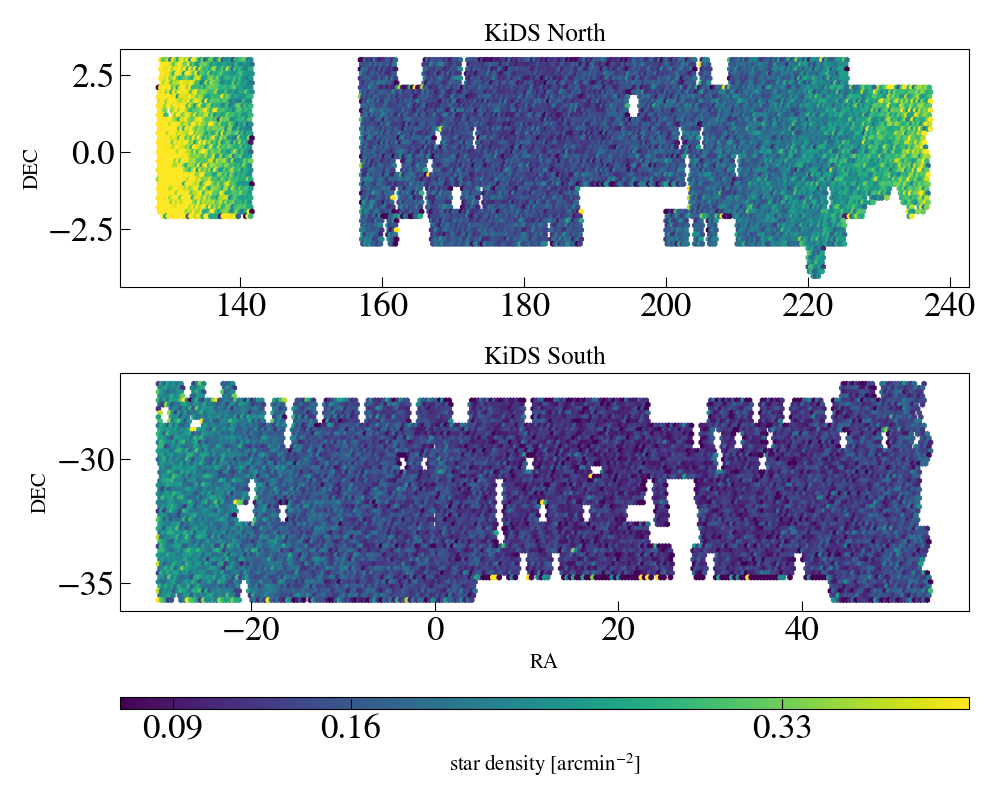
\includegraphics[width=0.7\textwidth, height = 0.5\textwidth]{figures_tmp/sys/scatter_nstar.png}
\caption{ The $\mathtt{HEALPIX}$ map of the density of GAIA DR2 stars ($14<G<17$) in the KiDS DR4 footprint.} 
\label{fig:scatter_stardens}
\end{figure*}

\begin{figure*}
\centering
\begin{tabular}{cc}
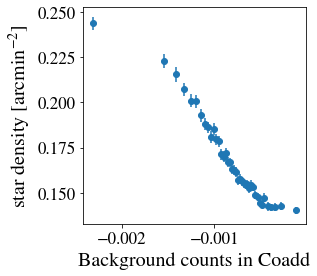
\includegraphics[width=0.4\textwidth, height =0.4\textwidth]{figures_tmp/sys_nstar_backgr.png}
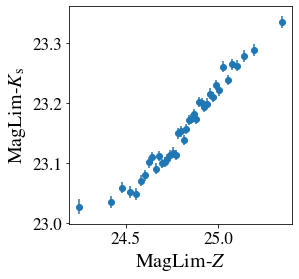
\includegraphics[width=0.4\textwidth, height =0.4\textwidth]{figures_tmp/sys_maglimk_maglimz.png}
\end{tabular}
\begin{tabular}{cc}
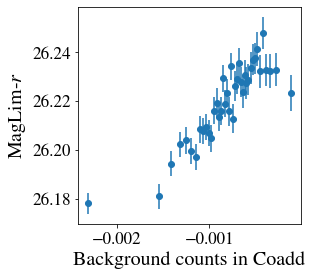
\includegraphics[width=0.4\textwidth, height =0.4\textwidth]{figures_tmp/sys_maglimr_backgr.png}
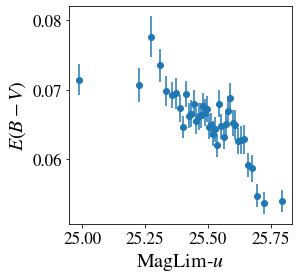
\includegraphics[width=0.4\textwidth, height =0.4\textwidth]{figures_tmp/sys_ext_maglimu.png}
\end{tabular}
\caption{ Demonstration of correlation between some of the survey properties. The anti-correlation between the background counts in the coadds and the stellar number density is evident (\textit{Top Left}). Furthermore, there is a correlation between the magnitude limits in the $Z$ and the $K_{\rm s}$ bands (\textit{Top Right}), a correlation between the background counts and the limiting magnitude in the $r$-band (\textit{Bottom Left}), and an anti-correlation between the limiting magnitude in the $u$-band and the galactic extinction (\textit{Bottom Right}).} 
\label{fig:sys_sys_correlation}
\end{figure*}


We consider a range of photometric systematics with on-sky variations that can impact the variations of galaxy number densities. In total we consider 13 survey properties that we further pixelate using $\healpix$ (\citealt{healpix}). We produce the $\healpix$ map of these properties with $n_{\rm side} = 256$. Moreover, we consider the Galactic extinction in the $r$-band, and the star number density in the survey footprint. 

It is important to note that the detection band in the KiDS photometry pipeline is the $r$-band. Therefore, most of the systematic parameters considered in our analysis are extracted from the $r$-band imaging data. Since we make use of the galaxy GAaP magnitudes and magnitude errors in our red-sequence pipeline, we also include the GAaP limiting magnitudes in our list of imaging systematics.  
 

In what follows, we list the set of systematic properties considered in our investigation:

\begin{itemize}

  \item \textbf{Background counts in the THELI images}: The background counts at the centroid positions of the objects in the THELI-processed $r$-band detection images. In KiDS DR4, the background count is provided as $\mathtt{BACKGROUND}$. Note that the THELI processed detection images are background subtracted. The $\mathtt{BACKGROUND}$ parameter simply returns the value of the residual sky background at the positions of objects, therefore the background `counts' could be also negative. %The healpix map of the background counts in shown in~ Figure\ref{fig:scatter_BackGr}.

  \item \textbf{Detection threshold above background}: This quantity is measured in units of counts and it is provided in the single-band source list as $\mathtt{THRESHOLD}$. 
  
  \item \textbf{Limiting magnitudes in 9 bands}: The limiting GAaP magnitude attributes are provided in DR4 as $\mathtt{MAG}\_\mathtt{LIM}\_\mathtt{band}$, where $\mathtt{band} = \{u,g,r,i,Z,Y,J,H,K_{\rm s}\}$. 
  For each band the limiting magnitudes are evaluated on an object-by-object basis. At the position of a given object, the limiting GAaP magnitude corresponds to the 1-$\sigma$ GAaP flux error for the aperture of the source. The aperture size is set to the optimal value of the minimum aperture $\mathtt{MIN}\_\mathtt{APER}$ in GAaP photometry. Thus, it depends on the pixel noise---in the Gaussianized image where the GAaP flux is measured---as well as the aperture size. This implies that the limitting magnitudes are indirectly dependent on the full-width-at half-maximum of the point spread function in the bandpass as well as the sky background counts.   
  
  \item \textbf{PSF full Width at half maximum (FWHM) in the $r$-band}: the PSF FWHM in the $r$-band measured in units of arcseconds. The PSF FWHM is calculated using the fallowing catalogue entries: $\mathtt{PSFe1}$, $\mathtt{PSFe2}$, and $\mathtt{PSF\_Strehl\_ratio}$.
    
  \item \textbf{PSF ellipticity in the $r$-band}: the KiDS PSF ellipticity in the $r$-band. As discussed in \citet{kuijken2019}, both PSF ellipticity and the PSF FWHM in the $r$-band are small, allowing for benign imaging variation in the $r$-band which is used as the detection band in the KiDS photometry pipeline. 
  The PSF ellipticity quantity is computed from the $\mathtt{PSFe1}$, $\mathtt{PSFe2}$ columns in the data. 
  
  \item \textbf{Galactic dust extinction in the $r$-band}: This quantity is provided as $\mathtt{EXTINCTION}\_r$ in the nine-band catalogue of KiDS DR4. The Galactic extinction in the other bands are given by scaling the extinction in the $r$-band (\citealt{schlegel98, schlafly2011}).
  
  \item \textbf{Star number density}: We determine the the stellar density from the pixelated number density map of bright stars in the second data release of GAIA (GAIA DR2, \citet{gaia0}). This is done by considering the GAIA stars with the $G$-band magnitude between 12 and 17. This is the magnitude range in which the GAIA DR2 G-band is complete (\citealt{gaia0,gaia1}). Note that only GAIA DR2 stars that lie in the KiDS footprint are considered in the process of generating the map of stellar number densities. 
  
  It is worth noting that a number of parameters in the KiDS DR4 catalogue are dedicated to star-galaxy separation. These include the $\mathtt{CLASS\_STAR}$
  parameter which is an output of the source extractor software, the $\mathtt{SG2DPHOT}$ parameter which is an internal KiDS star-galaxy classifier \citep[e.g.][]{kids_dr3, radovich2017}, and lastly the $\mathtt{SG\_FLAG}$ parameter which is derived based on an estimate of the size-peakiness relation of objects. Note that we have already excluded objects in our sample that are classified as high confidence stars according to the parameters $\mathtt{SG2DPHOT}$ and $\mathtt{SG\_FLAG}$. However, in order to reduce any impact of possible imperfections in the star-galaxy classification on our systematic tests, we decide to use a systematic map constructed from an external GAIA DR2 catalogue with a complete sample of stars. The $\mathtt{HEALPIX}$ map of star number densities is shown in Figure~\ref{fig:scatter_stardens}.
 
\end{itemize}

%\begin{figure*}
%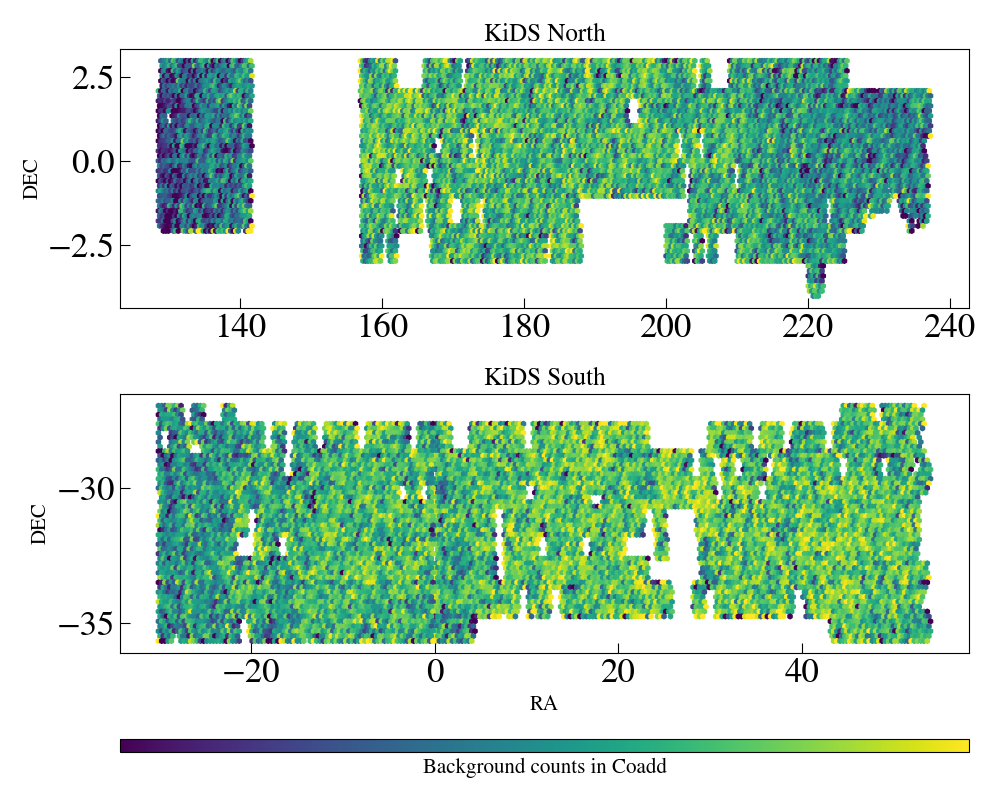
\includegraphics[width=\textwidth, height = 0.5textwidth]{figures_tmp/sys/scatter_BackGr.png}
%\caption{\label{fig:scatter_BackGr} The healpix map of the background counts in the coadded images in the $r$-band in the KiDS DR4 footprint.} 
%\end{figure*}


\begin{figure*}
\centering
    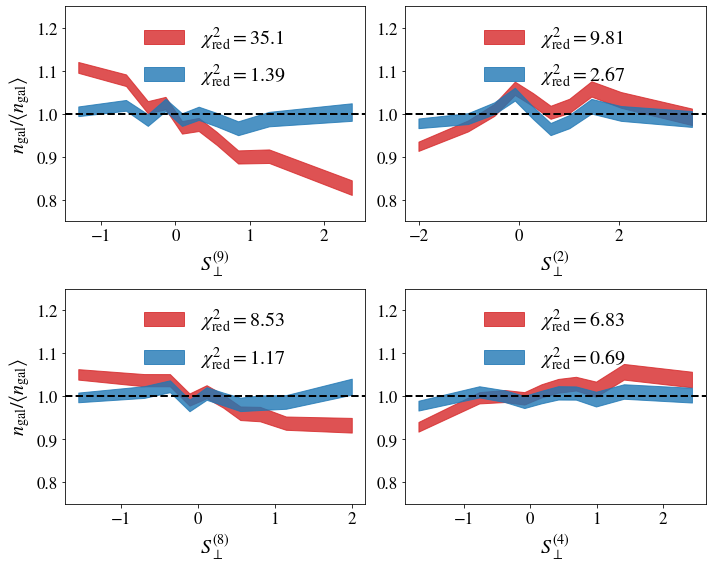
\includegraphics[width = 0.9\textwidth]{figures_tmp/weights_2.png}
    \caption{Variation of the galaxy over density versus the orthogonal systematic parameters $\{\mathbf{S}_{\perp}\}$ in the third redshift bin $z_{\rm red} \in [0.45, 0.6]$ with (shown in blue) and without (shown in red) the systematic weights included. The deviation of the galaxy over density from unity is quantified by $\chi^{2}_{\rm red}$. Note that we have only included the four components of $\{\mathbf{S}_{\perp}\}$ that induce the most signifcant variations in the observed galaxy number densities (shown in red). After including the photometric weights (shown in blue) the systematic trends are reduced significantly.}
    \label{fig:sys_ng_correlation}
\end{figure*}

\begin{figure}
    %\centering
    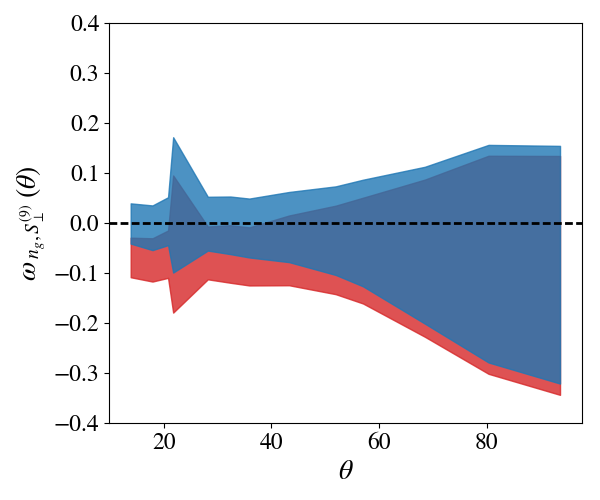
\includegraphics[width = \columnwidth, height =\columnwidth]{figures_tmp/cross_45.png}
    \caption{Cross correlation of the galaxy number density in the third redshift bin with the systematic variable most correlated with $n_g$. The cross-correlation is computed with (without) the systematic weights is shown in blue (red). The width of the bands show the 68\% in the jacknife uncertainties. The estimated cross-correlations are consistent with zero.}
    \label{fig:cross-correlation}
\end{figure}


\subsection{The impact of photometric systematics}

%\mb{[the same was already said in sec.4.1]}
%In order to quantify such systematic-induced variations, we make pixelated on-sky maps of survey properties using the $\mathtt{HEALPIX}$ framework (\citealt{healpix})\footnote{In particular, we use healpy (\citealt{healpy2019}), a python library for handling and analyzing healpix maps.}. 
Similar to the works of \citet{ross2017, rezaie2019}, we construct the pixelated maps with the resolution of $N_{\rm side} = 256$. 

The systematic parameters considered in our investigation are correlated. Figure~\ref{fig:sys_sys_correlation} demonstrates the correlation between various systematic parameters in the survey. For instance, there is a strong anti-correlation between the background counts in the $r$-band and the stellar number density, and an anti-correlation between the magnitude limit in the $u$-band and the galactic extinction $E(B-V)$. Conversely, there is a strong correlation between the background counts in the $r$-band and the $r$-band limiting magnitude, and between the $Z$-band and the $K_{\rm s}$ band limiting magnitudes. 

The anti-correlation between the background counts and the stellar number density stems from the tendency of the image processing pipeline to over-estimate, and as a result, to over-subtract the sky background in the fields with higher stellar density. The correlation between the limiting magnitudes of the infrared bands is due to the observing strategy of the VIKING survey according to which, all the infrared band data were taken simultaneously, which is different from the KiDS $ugri$ case, where each band was observed independently.

Due to the covariance between various imaging systematics, we inspect the variation of the observed galaxy number densities and the imaging systematics in the linear basis in which the covariance matrix between the systematic parameters is diagonal. The basis vectors of this space are the eigen-vectors of the covariance matrix of imaging systematics, or equivalently the principal components of the imaging systematics\footnote{Without excluding any of the principal components due to low contribution to the variance present in the space of imaging systematics.}. In such a basis, one can assess the variations between the observed galaxy number density and the different basis vectors independently. 

In particular, we inspect the variation of galaxy over-densities $\delta_{\rm gal} = N_{\rm gal}/\langle N_{\rm gal} \rangle$. Any deviation of this quantity with respect to unity as a function of an imaging systematic will signal a non-vanishing impact of that imaging systematic\footnote{Note that alternatively, one can reformulate this by looking at the deviations of $N_{\rm gal}/N_{\rm random}$ (modulo some normalization) from unity, where $N_{\rm random}$ is the number density of a set of uniformly distributed random points across the survey footprint \citep[e.g. ][]{bautista2018sdss, icaza2020clustering}.}.
Let us denote the list of all pixelated systematic parameters by $\{\mathbf{s}_{i} \in \mathbb{R}^{15}\}_{i=1}^{N_{\rm pix}}$ where the subscript $i$ denotes the position of the pixel $i$ on the sky. Furthermore, we transform the set of vectors 
$\{\mathbf{s}_{i} \in \mathbb{R}^{15}\}_{i=1}^{N_{\rm pix}}$ so that the mean and the variance across each of the 15 dimensions are zero and one, respectively. Afterwards, we transform this 15 dimensional linear basis to a new orthogonal basis in which the covariance matrix of the systematic vectors is diagonal. In this new basis, we represent the list of systematic parameters by $\{\mathbf{S}_{\perp,i} \in \mathbb{R}^{15}\}_{i=1}^{N_{\rm pix}}$ where at each pixel we have:

\begin{equation}
    \mathbf{S}_{\perp} = [S_{\perp}^{(1)}, S_{\perp}^{(2)}, ..., S_{\perp}^{(15)}],
\end{equation}
where $S_{\perp}^{(j)}$ is the $j$-th systematic vector in the new basis. For the third redshift bin\footnote{For brevity we only show the systematic-density trends in the third bin. The systematic trends in the rest of the redshift bins and the corrections are similar.} $z_{\rm red} \in [0.45, 0.6]$, the variation of the observed number density versus the systematic parameters $\mathbf{S}_{\perp}$ is shown by the red bands in Figure~\ref{fig:sys_ng_correlation}, where we only show the four most significant variations quantified by the reduced chi-squared $\chi^2_{\rm red}$. A higher $\chi^{2}_{\rm red}$ value implies a more considerable systematic trend in which the observed galaxy over-density deviates from unity.  

%Note that the observed galaxy number density-systematic trends are shown with the orange errorbars. In each row, only the trends with considerable deviation from unity are shown. We note that the variations in the observed number density as a result of survey inhomogeneity changes depends on the galaxy sample under study,  with galaxies in different tomographic bins showing different sensitivities.

In this work we mitigate the impact of systematics by introducing a set of photometric weights to remove the systematic-induced variation of galaxy densities due to imaging systematics. This approach has been widely utilized in galaxy clustering analyses in order to account for the impact of systematics: the clustering of LRGs in SDSS BOSS (\citealt{ross2012clustering, ross2017clustering}), galaxy clustering in the Dark Energy Survey (\citealt{elvin2017,crocce2019dark}), DESI legacy survey (\citealt{DESI_systematic}), and finally clustering of LRGs in SDSS-eBOSS (\citealt{bautista2018sdss, icaza2020clustering}). 

Following the work of \citet{bautista2018sdss}, we introduce a set of photometric weights by assuming a relation between the pixelated observed galaxy overdensities and $\delta_{\rm gal} = N_{\rm gal}/\langle N_{\rm gal}\rangle$ and the set of pixelated systematic parameters. In \citet{bautista2018sdss} this relation is assumed to be linear, i.e. $\boldsymbol{\delta}_{\rm gal} = \mathbf{Ws+b} + \mathbf{\mathrm{noise}}$. 

Additionally, we consider two modifications. First, we introduce a set of second-order polynomial features from the original feature space $\{\mathbf{s}\}$. These polynomial features are then mapped to the observed galaxy overdensity via a linear relation. Furthermore, we introduce an $L_{2}$ regularization to this regression problem which is implemented by adding a regularization term $\lambda \sum_{k} W_k^2$ to the least square cost function. The added advantage of this regularization term is that it tends to keep the $\mathbf{W}$ parameters small thereby avoiding overfitting.

In practice, we choose the regularization hyper-parameter $\lambda$ by a $k$-fold cross-validation search in which we explore a wide range of $\lambda$ values from $10^{-4}$ to $10^{5}$. We note that in all the redshift bins, our cross-validation optimization procedure prefers a heavy regularization in which a very large value of $\lambda \in [10^3-10^5]$ is favored. The advantage of this approach to that of \citet{ross2017clustering} is that it does not assume that there is no correlation between the systematic parameters.

The prediction of this model, once applied to the pixelated systematic maps provides a set of photometric weights that removes the systematically induced variations in the galaxy number density. The photometric weights are obtained by taking the inverse of the prediction of the model. Figure~\ref{fig:sys_ng_correlation} demonstrates how the photometric weights derived from our framework can help reduce the systematic trends seen in the observed galaxy number densities. In Figure~\ref{fig:sys_ng_correlation}, the density-correlations are displayed after taking into account the photometric weights (shown in blue) and without the photometric weights (shown in red). We note that the reduced $\chi^{2}$ is reduced significantly once the photometric weights are taken into consideration. 

Moreover, we investigate the two-point cross-correlations of the galaxy number density and the orthogonal systematic parameters $\{\mathbf{S}_{\perp, i}\}_{i=1}^{N_{pix}}$ as a function of angular separation. In Figure~\ref{fig:cross-correlation}, the cross-correlations between the galaxy number density in the third redshift bin ($z_{\rm red} \in [0.45, 0.6]$) and  the systematic vector $S_{\perp}^{(9)}$ with the largest correlation with the observed density (see Figure~\ref{fig:sys_ng_correlation}) is shown in two cases: the case where we include the systematic weights (shown in blue) and where we do not include the systematic weights (shown in red). The width of the bands represent the 68\% uncertainties obtained from the jackknife method. In both cases, we note that the cross-correlations are consistent with zero with slight improvements when the photometric weights are accounted for.

Alternatively, one can use self organizing maps (SOM, \citealt{kohonen1997}) for learning the systematic galaxy density modes due the variable survey properties and then generating a set of organized randoms mimicking the galaxy depletion pattern across the survey footprint. We have also tested this method and we found that this method works best in correcting the systematic depletion in a galaxy sample with a higher number density than the galaxy sample in our study. This approach is being pursued by Johnston et al.(in prep) to mitigate the systamtic biases in clustering of galaxies in the KiDS DR4 bright sample.
%\mb{[mention that this is what Johnston in prep. will discuss for the general bright sample?]}

We have not explored the effect of various observing conditions on the distribution of the physical properties of the galaxies. Such effects can in principle generate systematic on-sky variations of the estimate host halo mass of galaxies in our sample. Such an effect can subsequently further complicate the cosmological analysis. This problem is exacerbated in a galaxy survey covering a larger area and can only be taken into account through a careful forward model approach which is outside the scope of this paper.  




%\begin{table}
%\begin{center}%
%	\caption{{\bf Prior probability distribution over the model parameters:} 
%    The prior probability distribution over the linear galaxy bias and the photo-z shift parameters. We assume a uniform prior over the bias parameters and a Gaussian prior over the photo-z shift parameters. The Gaussian priors have zero means and variances set by the uncertainty on the mean redshifts of the DIR redshift distributions (see Table~\ref{tab:pz}).}
%	\label{tab:prior}
%%	\\	\hline
%		Parameter        & & Prior       & & Range \\
%		\hline
%		$b_{g}^{(i)}$    & & Uniform     & & $\mathcal{U}\Big(1,3.5\Big)$  \\
%		$\Delta z^{(i)}$ & & Gaussian    & & $\mathcal{N}\Big(0, \delta^{2}_{z^{(i)}}\Big)$  \\
%		\hline
%	\end{tabular}
%\end{center}
%\end{table}



\section{Galaxy Clustering}\label{sec:clustering}

\subsection{Theory}

Assuming a local deterministic linear galaxy bias, the galaxy overdensity $\delta_g$ is related to the matter overdensity $\delta_m$ through a linear relation: $\delta_g = b_g \delta_m$, where the parameter $b_g$ is the linear bias parameter. Such assumption is expected to hold on sufficiently large scales \citep[e.g.][]{Kravtsov1999, marian2015}, whereas on small scales, the nonlinear structure formation is best described by the more sophisticated halo model \citep[e.g. ][]{berlind2002,cooray2002,zehavi2011,hand2017,vakili_hahn}.

Assuming a nonlinear matter power-spectrum $P_{\delta}(k,z)$, and a galaxy population described by linear bias of $b_g$, and redshift distribution of $n_g(z)$, one can predict the angular two-point correlation function $w_{g}(\theta)$. Under the Limber, flat-sky approximations (\citealt{limber1961, loverde2008, kilbinger2017, kitching2017}), the angular clustering $w_g(\theta)$ is given by:

\begin{eqnarray}
w_{g}(\theta) &=& b_g^2 \int_{0}^{\infty} \frac{2\pi dl}{l}J_{0}(l\theta)  \nonumber \\ 
            &\times& \int_{0}^{\chi_{\rm H}} d\chi_{\rm c} \Big[\frac{n_{g}(z)\frac{dz}{d\chi_{\rm c}}}{\chi_{\rm c}}\Big]^{2}P_{\rm NL}\Big(\frac{l+1/2}{\chi_{\rm c}}; z\Big),                  
\label{eq:clustering_theory}
\end{eqnarray}
where $\chi_{\rm c}$ is the comoving distance, $P_{\rm NL}$ is the analytical nonlinear power spectrum evaluated at the wave-number $k = \frac{l+1/2}{\chi_{\rm c}}$ and redshift $z$. The nonlinear power spectrum can be calculated using different recipes such as the halo model \citep[e.g. ][]{takahashi2012, mead2015, smith2019}, or emulation \citep[e.g.][]{emu2014}. Hereafter we use the Core Cosmology Library ($\mathtt{CCL}$, \citealt{ccl2019, ccl_code}) to compute the theoretical predictions of angular clustering. For our choice of nonlinear power spectrum, we use the~\citet{takahashi2012} model as it is capable of predicting the matter clustering in the linear and quasi-linear regimes (i.e. $\chi_{\rm c}>8 \; \mathrm{Mpc}/h$) considered in this study.

We calculate the theoretical prediction (\ref{eq:clustering_theory}) for all four tomographic bins in our galaxy sample with their corresponding linear bias parameters $\{b^{(i)}_{g}\}_{i=1}^{4}$ and redshift distributions $\{n^{(i)}_{g}(z)\}_{i=1}^{4}$.

Assuming a fixed cosmology, we aim to estimate the linear bias parameters $\{b^{(i)}_{g}\}_{i=1}^{4}$ by fitting the theoretical prediction (\ref{eq:clustering_theory}) to the angular clustering measurements provided in Section~\ref{sec:measurement}. It is worth noting that one major source of systematic in this theoretical prediction is the uncertainty on the mean of the redshift distributions $\{n_{g}^{(i)}(z)\}_{i=1}^{4}$. In order to mitigate the impact of such systematic, we assume that the estimated redshift distribution at each tomographic bin $n_{g}^{(i)}(z)$ is effectively given by shifting the underlying unbiased redshift distribution $n_{g, \rm true}^{(i)}(z - \delta z^{(i)})$, where the parameter $\delta z^{(i)}$ is the uncertainty on the mean of the redshift distribution of $i$-th redshift bin. In Section~\ref{sec:inference} we will 
discuss how the uncertainty over the mean of the redshift distribution can be estimated. When reporting the constraints on the galaxy bias parameters, we marginalize over the redshift uncertainties. 

\subsection{Clustering measurements}\label{sec:measurement}

The galaxy two-point correlation function is the excess probability, compared to random, of finding a pair of galaxies within a given angular or physical separation. Given that we do not know the exact redshifts of the galaxies, we focus on computing the angular correlation function which can be obtained by performing pair-counts in angular bins perpendicular to the line of sight. We measure the angular clustering using the Landy-Szalay estimator (\citealt{landy}):
\begin{equation}
    \widehat{w}(\theta) = \frac{DD-2DR+RR}{RR},
\label{eq:landy}
\end{equation}
where $DD$ denotes the number of galaxy pairs within an angular separation bin centered at $\theta$, $DR$ denotes the number of galaxy-random pairs, and $RR$ denotes the number of random pairs. 

As discussed in Section~\ref{sec:systematic}, in each redshift bin a photometric weight is assigned to each galaxy depending on the its position on the sky. These weights are derived such that the on-sky variations of galaxy overdensity due to survey properties are mitigated. We compute two sets of angular clustering measurements, one with the photometric weights, and another without the photometric weights. 

\begin{figure*}
\centring
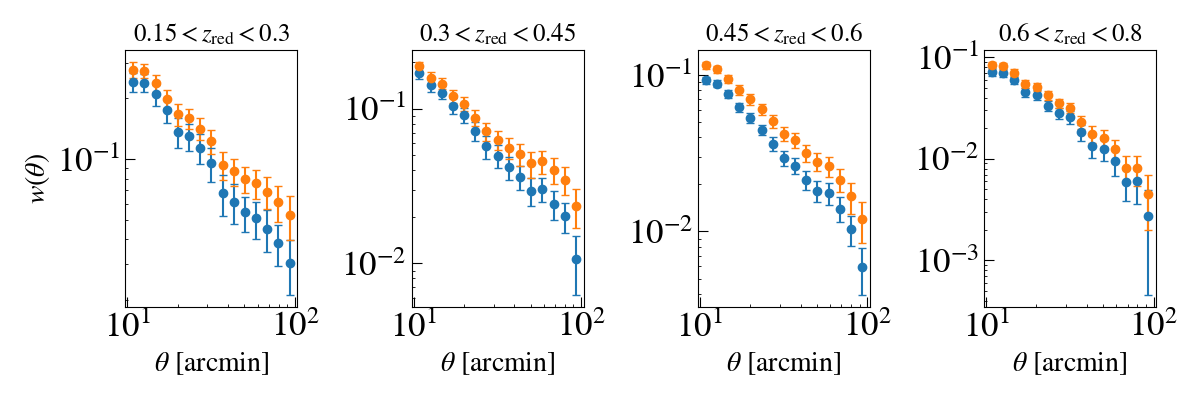
\includegraphics[width=0.9\textwidth]{figures_tmp/woftheta.png}
\caption{Clustering measurements for the four redshift bins. In each panel, the blue (orange) data-points correspond to the correlation functions computed with (without) the systematic weights.} 
\label{fig:xi} 
\end{figure*}

The angular clustering measurements of LRGs at four tomographic bins are displayed in Figure~\ref{fig:xi}, with the first three bins encompassing the galaxies in the dense $(L> 0.5L_{\star})$ sample and the last bin ($0.6<z<0.8$) encompassing the galaxies in the luminous $(L> L_{\star})$ sample. The clustering signal estimated with (without) the photometric weights is shown in blue (orange). The correlation functions are measured in 15 logarithmically-spaced bins in the range $ 10\leq \theta \leq 100 \; \mathrm{arcmin}$. 

We estimate the measurement uncertainties using the jackknife resampling method (\citealt{norberg2009,oliver2016,singh2017,shirasaki2017}). 
In this method, the survey footprint is first divided into $N_{\mathrm{JK}}$ jackknife subsamples of approximately equal area\footnote{The segmentation of KiDS DR4 footprint into $N_{\mathrm{JK}}$ is done with the $K$-means algorithm. In particular we made use of the implementation of this algorithm designed to handle RA and DEC coordinates on the sky (\hyperlink{kmeans\_radec}{https://github.com/esheldon/kmeans\_radec})}.
For each subsample $k\in\{1,...,N_{\mathrm{JK}}\}$, the clustering data vector  
is measured by dropping the $k$-th subsample and estimating the clustering signal of the rest of the survey area. Note that $\boldsymbol{w}_{g}^{(k)}$ is a vector containing the correlation function measured in all the 15 angular bins considered in this study. The jackknife estimator of the covariance matrix is then given by:
\be 
\widehat{C}_{\rm JK} = \frac{\njk - 1}{\njk}\sum_{k=1}^{\njk}\big(\dk-\dbar\big)^{T}\big(\dk-\dbar\big), 
\label{eq:jk}
\ee
where $\dbar$ is the mean of all $\boldsymbol{w}_{g}^{(k)}$ vectors. 


Since the covariance matrix is estimated from the jackknife method with a finite number of jackknife subsamples, our estimate of the covariance matrix and its inverse are noisy. The unbiased estimate of the inverse covariance matrix is related to the inverse of the estimated jackknife covariance matrix $\hat{C}_{\rm JK}$ following \citet{hartlap2007}:

\be
\widehat{C^{-1}} = \frac{\njk - N_{\rm d} - 2}{\njk - 1} \widehat{C}^{-1}_{\rm JK},
\label{eq:hartlap}
\ee
where $\njk$ is the number of jackknife subsamples and $N_{\rm d}$ is the number of bins, in the clustering measurements, that enter the likelihood function evaluation. In other words, the data points that do not pass the scale cuts described in section~\ref{sec:inference} are excluded from the Equation~\ref{eq:hartlap}.  

\begin{figure*}
\centering
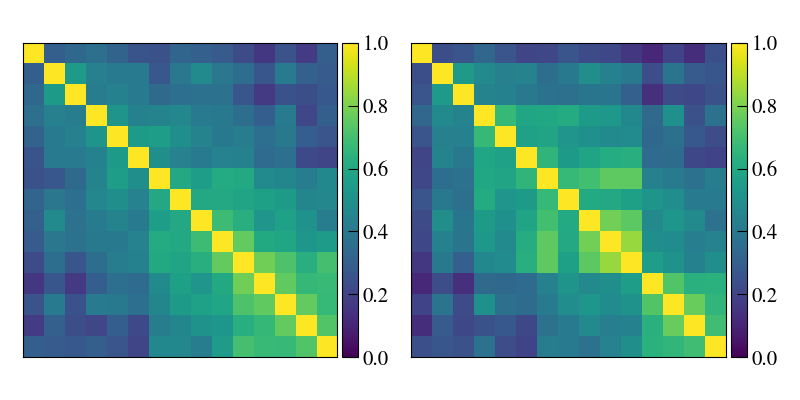
\includegraphics[width=0.9\textwidth]{figures_tmp/correlation_last_bin_cosmo.png}
\caption{ Two correlation matrices corresponding to the angular clustering measurements in the last tomographic bin. One of the matrices is the original correlation matrix derived from the jackknife covariance matrix computed in section~\ref{sec:measurement}, while the other matrix is constructed with the method of~\citet{sellentin2019} such that the posterior probability is shifted.} 
\label{fig:blind}
\end{figure*}

\subsection{Inference setup}\label{sec:inference}

\subsubsection{Parameters}

In order to fit the theoretical model of angular clustering to the data, we need to clarify our choices of parameters. Assuming a fixed cosmology, we estimate the linear galaxy bias (using equation~\ref{eq:clustering_theory}) of the red galaxies in the redshift tomographic bins. We estimate the bias parameters by marginalizing over the photometric redshift uncertainty parameters.  
Furthermore, we choose a flat LCDM model assuming $\Omega_m = 0.25, \;\Omega_{\Lambda} = 0.75, \; \Omega_b = 0.044, \; \sigma_{8} = 0.8, \; n_s = 0.95, \; h = 0.7$. Our choice is consistent with the 
%MICE suite of cosmological simulations (\citealt{MICE1}). The simulation's input cosmology is consistent with the 
best-fit flat $\Lambda$CDM cosmology given the WMAP5 data (\citealt{WMAP5}). It is important to note that due to the correlation between amplitude of the nonlinear matter power spectrum, proportional to $S_8 = \sigma_8(\Omega_m)^{(1/3)}$ parameter, and the linear galaxy bias, our constraints will depend on the assumed cosmology.

%\mb{[but you never use MICE here anyway?]}

%These parameters are denoted by $\{b^{(1)}_g, \; b^{(2)}_g, \; b^{(3)}_g, \; b^{(4)}_g\}$. 

%Furthermore, we keep our estimates of the photometric redshift distributions fixed. That is, we do not marginalize over photo-$z$ uncertainties. 
%\mjv{I'm running new chains to marginalize over photo-z errors!}
%In our future 3x2pt analysis however, we will jointly constrain the cosmological parameters, linear galaxy bias, as well as photometric redshift uncertainties of our sample. 


We adopt the following priors over the model parameters. For the galaxy bias parameters, we assume a uniform prior with a lower bound of 1 and an upper bound of 3. For the prior distribution of the photo-z shift parameters $\{\delta z _{i}\}_{i=1}^{4}$ we assume a Gaussian distribution with zero mean and a dispersion which we estimate in the following way. We assume that there are two major contributions to the uncertainty of the mean of the redshift distributions. The first contribution is the spatial sample variance which we compute using the jackknife resampling method. The second contribution is estimated by computing the covariance between the photo-z biases with respect to the four spectroscopic redshift surveys considered in this study (see Table~\ref{tab:bias}). Combining these two sources of uncertainty will provide us with an estimate of the prior distribution over the photo-z shift parameters:
\begin{equation}
    \delta z_{i} \sim \mathcal{N}\big(0, \sigma_{\delta z_{i}}\big),
\end{equation}
where $\sigma_{\delta z_{i}}$ is $2.4\times 10^{-3}$, $3.2\times 10^{-3}$, $2.3\times 10^{-3}$, and $4.6\times 10^{-3}$ for the first, second, third, and fourth redshift bins respectively. 

\subsubsection{Blinding}

In order to avoid confirmation bias we adopt the blinding scheme introduced in \citep{sellentin2019}. In this approach the blinded element of the inference pipeline is the inverse covariance matrix as opposed to the catalogues (\citealt{hendrick2017}), photo-z distributions (\citealt{hendrik2020}), or the correlation functions (\citealt{muir2019}). 

In this approach the estimated inverse covariance matrix is changed by multiplication of a diagonal matrix to the Cholesky decomposition of the estimated inverse covariance matrix\footnote{The Cholesky decomposition of a symmetric positive-definite matrix $A$ is a matrix factorization that can be expressed as $A = LL^{\rm T}$, where $L$ is a unique lower triangular matrix.}. The diagonal matrix is chosen such that the posterior distributions derived from the new inverse covariance matrix are shifted with the respect to those estimated from the fiducial inverse covariance matrix. Transformation of the inverse covariance matrix is given by the following set of equations:

\begin{eqnarray}
\widehat{C^{-1}} &=& L^{T}L \\
             &\rightarrow& L^{T}B^{T}BL, \label{eq:blinded}
\end{eqnarray}
where $L^{T}L$ is the Cholesky decomposition of the original inverse covariance matrix, $B$ is the diagonal matrix responsible for shifting the peak of the posterior probability distribution, and $L^{T}B^{T}BL$ is the blinded inverse covariance matrix.

Figure~\ref{fig:blind} demonstrates the described blinding scheme, where the two panels show the correlation matrix of the clustering measurement corresponding to the last redshift bin before and after blinding.

\subsubsection{Scale cuts}\label{sec:scale_cut}

The theoretical model summarized in equation~\ref{eq:clustering_theory} fails to capture the full complexity of the galaxy-matter connection on small scales as it relies only on a simple linear deterministic treatment of galaxy bias. Therefore, we decided to apply a conservative cut on the comoving scales considered in our theoretical modeling of the clustering signal. In particular, we adopt a cut at a comoving scale of 8 $\mathrm{Mpc}h^{-1}$ which translates to a minimum angular scale (hereafter denoted by $\theta_{\rm min}$) of 28.3 arcmin for the first bin, 18.4 arcmin for the second bin, 13.7 arcmin for the third bin, and finally 10.8 arcmin for the last redshift bin. The comoving distance is converted to angular scales assuming the flat $\Lambda$CDM cosmology discussed shortly above. Furthermore, the parameter $\theta_{\rm min}$ in each tomographic bin is calculated from the comoving distance at the mean redshift of the redshift bin.

 
 

\subsubsection{Likelihood and posterior sampling}

With the theoretical model, the measurements, and the blinded covariance matrix at hand, now we are ready to constrain the linear galaxy bias and photo-z distribution shift parameters for each redshift bin: $\{b_{g}^{(i)}, \delta z^{(i)}\}_{i=1}^{4}$. 

%The assumed prior probability over these parameters is specified by Table~\ref{tab:prior}. 
%The assumed prior probability over the linear galaxy bias parameters is assumed to be a uniform distribution with lower and upper bounds of 1 and 3.5. The prior over the photo-z shift parameters $\{\Delta_{z^{(i)}}\}_{i=1}^{4}$ is assumed to be a normal distribution with mean 0 and a standard deviation $\delta_z^{(i)}$.  In each bin, the parameter $\delta_z^{(i)}$ is found in the following way. First we perform bootstrap resampling of the scaled redshift residuals and then for each sample we compute its corresponding set of student-t distribution parameters. Each set of parameters correspond to a redshift distribution for the redshift bin. The scatter between the mean values of these redshift distributions provides an estimate of the parameter $\delta_z^{(i)}$.

We assume that the likelihood, the probability of the data conditioned on the model parameters $p(d|\theta)$, is a multivariate Gaussian distribution with the mean given by the theoretical prediction (Eq.~\ref{eq:clustering_theory}) and with the inverse covariance given by the blinded inverse covariance matrix (Eq.~\ref{eq:blinded}). The model parameters are constrained by MCMC sampling from the posterior probability distribution $p(\theta | d) \propto p(d|\theta)p(\theta)$ using the $\mathtt{emcee}$ implementation (\citealt{emcee}) of the affine-invariant ensemble Markov Chain Monte Carlo sampling method of~\citet{goodman2010}.


\subsection{Constraints}

Figure~\ref{fig:w_estimate} demonstrates the 68\% and 95\% posterior predictions of $w_{\theta}$ for all the four redshift bins. Given the blind uncertainties, the model predictions are consistent with the measurements. 
The 1$\sigma$ and $2\sigma$ levels of the 2D posterior surfaces in the $(b_g, \delta_z)$ parameter space as well as the marginalized distributions over the individual parameters are displayed in Figure~\ref{fig:joint_estimate}. With the exception of the first tomographic bin, the correlation between the inferred bias parameter and the photo-z shift parameter appears to be very low. The Spearman correlation between the two parameters is 0.6, 0.07, 0.05, and 0.1 for the four bins in increasing redshift order. 

The marginalized distributions are summarized in Table~\ref{tab:constraints}. We note that the constrains on the photo-z shift parameters are consistent with zero and largely consistent with the adopted priors over these parameters. Furthermore, we find consistency, given the uncertainties, between the constraints on the galaxy bias parameters of the first three bins. Note that the first three bins are constructed from the dense galaxy sample which has an approximately constant comoving density. On the other hand, our constraint on the bias parameter of the last bin is larger than those of the first three bins. This is expected as the  last bin is constructed from the luminous sample which consists of brighter galaxies residing in higher mass halos.

\begin{table}
	\centering
	\caption{\textbf{Summary of parameter constraints}: Model parameter constraints and uncertainties derived from the median and the 68\% confidence intervals of the marginalized posterior distributions}
	\label{tab:constraints}
	\begin{tabularx}{0.8\columnwidth}{lcr} % four columns, alignment for each
		\hline
		Redshift bin & $b_g$ & $\delta_z$\\
		\hline
		$0.15<z_{\rm red}<0.3$ & $1.78^{+0.02}_{-0.02}$ & $-0.00004^{+0.002}_{-0.002}$\\
		$0.3<z_{\rm red}<0.45$ & $1.89^{+0.11}_{-0.11}$ & $-0.0001^{+0.003}_{-0.003}$ \\
        $0.45<z_{\rm red}<0.8$ & $1.80^{+0.05}_{-0.05}$ & $0.0002^{+0.002}_{-0.002}$\\
        $0.6<z_{\rm red}<0.8$ & $2.07^{+0.06}_{-0.06}$ & $0.0005^{+0.005}_{-0.004}$\\
		\hline
	\end{tabularx}
\end{table}

In the default setup for studying the large-scale structure, we have relied on four redshift bins, three of which are constructed from the dense sample with bins defined by the redshift edges of [0.15, 0.3, 0.45, 0.6], and one last bin constructed from the luminous sample within the [0.6, 0.8] redshift interval. In order to assess the redshift-dependence of the estimated bias parameters we define two additional tomographic bins for the galaxies in the luminous sample with the redshift edges of [0.2, 0.4, 0.6]. Following the steps we have discussed for our fiducial large-scale structure analysis, we perform redshift estimation, photometric weight assignment, correlation function measurement, and blinding for the two new redshift bins in the luminous sample.  

The redshift-dependence of the bias is shown in Figure~\ref{fig:b_estimate}, where the estimated bias parameters of the luminous (dense) sample are shown in red (blue). The boxes mark the 68\% as well as the 95\% confidence intervals in the marginalized bias distributions. We note that within each sample, the bias constraints do not appear to have any strong redshift evolution. 

We compare our findings with the passive evolution model of galaxy bias (see \citealt{Fry1996, Tegmark1998}). The passive evolution model has been tested against the amplitude of the clustering of LRGs in \citet{Rita2012, Guo2013}\footnote{In particular, \citet{Guo2013} investigated the evolution of bias of red-galaxies for various ranges of constant comoving density, absolute magnitude, as well as colour.}. Following the approach of \citet{Guo2013} we fit the passive evolution model to our estimated biases as a function of redshift in two samples.   

Let us start by describing the bias evolution of the luminous sample. By fitting the passive evolution model of \citet{Fry1996} to the bias constraints in the luminous sample we find that this model provides a good picture of the evolution of galaxy bias yielding a $\chi^2/\mathrm{dof}$ of 0.73/2. When constraining the passive evolution model with the bias estimate of the highest redshift bin ($0.6<z_{\rm red}<0.8$), we find that the expected bias parameters for the first and the second bins to be 1.89 and 1.98 which are consistent with the estimated parameters (from the clustering measurements) of $1.97\pm0.19$ and $2.05\pm 0.075$ at 0.4$\sigma$ and 1$\sigma$ levels respectively. 

Turning our attention to the dense sample, we find that the passive evolution model provides a less consistent picture of bias evolution with a $\chi^2/\mathrm{dof}$ of 2.8/2. Once we condition the passive evolution model on the bias constraint of the highest redshift bin ($0.45<z_{\rm red}<0.6$), we find that the expected bias values for the first and the second redshift bins are 1.7 and 1.75 which are in disagreement with the inferred bias parameters (based on clustering measurement) of $1.78\pm0.02$ and $1.89\pm 0.11$ at $4.2\sigma$ and $1.3\sigma$ levels. 

\begin{figure*}
\centering
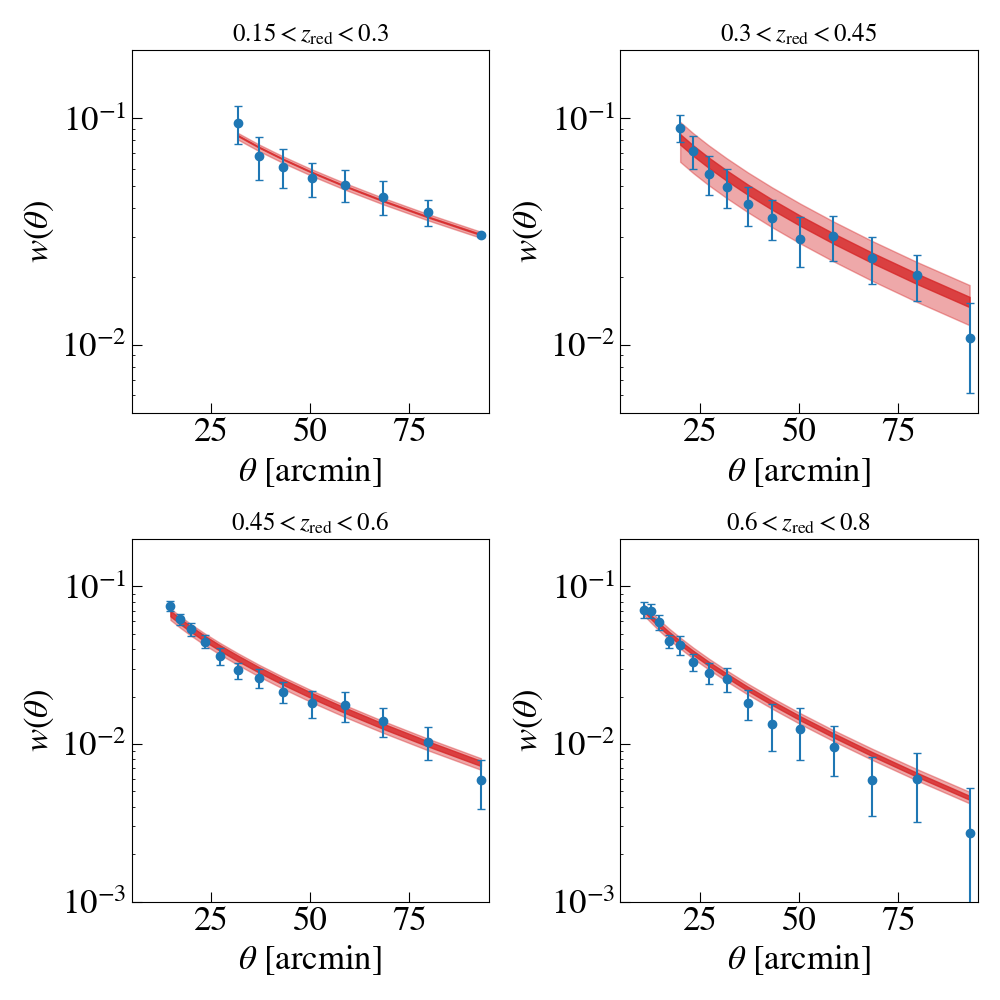
\includegraphics[width=0.9\textwidth]{figures_tmp/w_estimate.png}
\caption{ Comparison between the posterior predictions (red shaded) of clustering and the clustering measurements (blue) in the four tomographic bins. The dark and light shaded regions mark the 68\% and the 95\% confidence intervals. The error bars are derived from the diagonal elements of the blinded covariance matrix of the observations. } 
\label{fig:w_estimate}
\end{figure*}


\begin{figure}
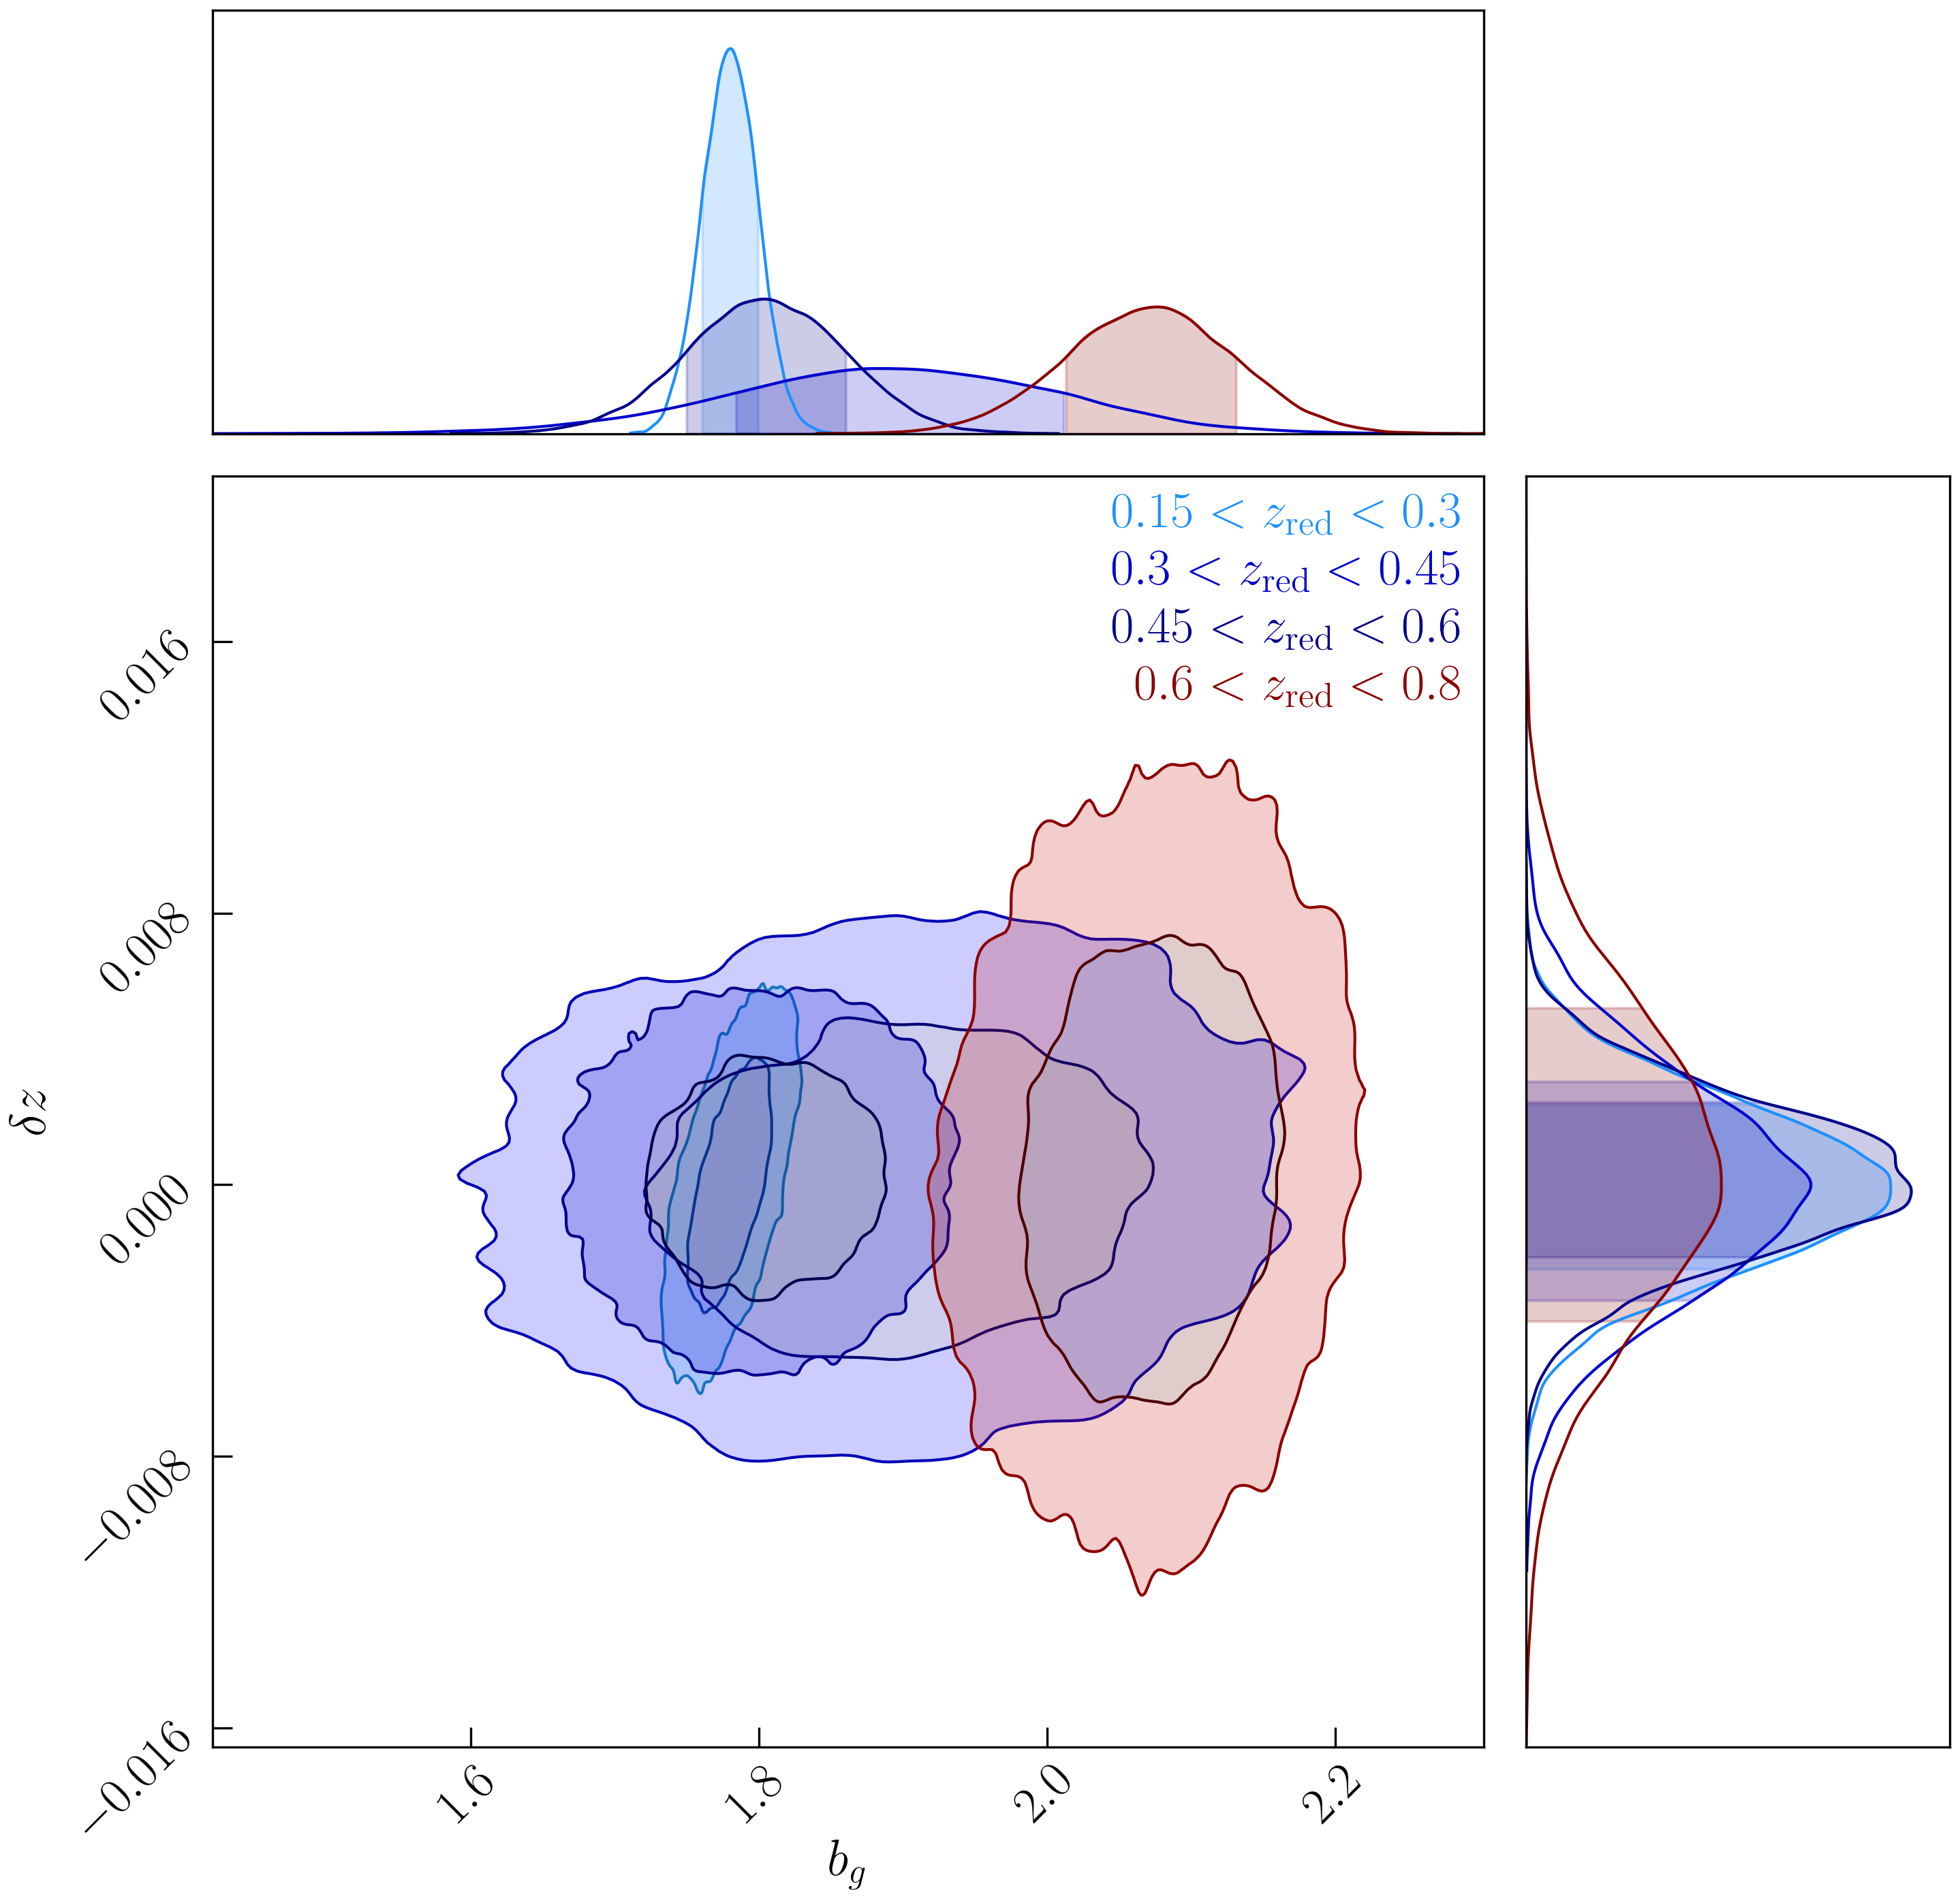
\includegraphics[width=\columnwidth]{figures_tmp/joint_estimate.png}
\caption{ Joint constraints on the linear galaxy bias and photo-z shift parameters shown for the redshift bins constructed with the dense sample (blue contours) and the last redshift bin which is constructed from the luminous sample (red contour).} 
\label{fig:joint_estimate}
\end{figure}

\begin{figure}
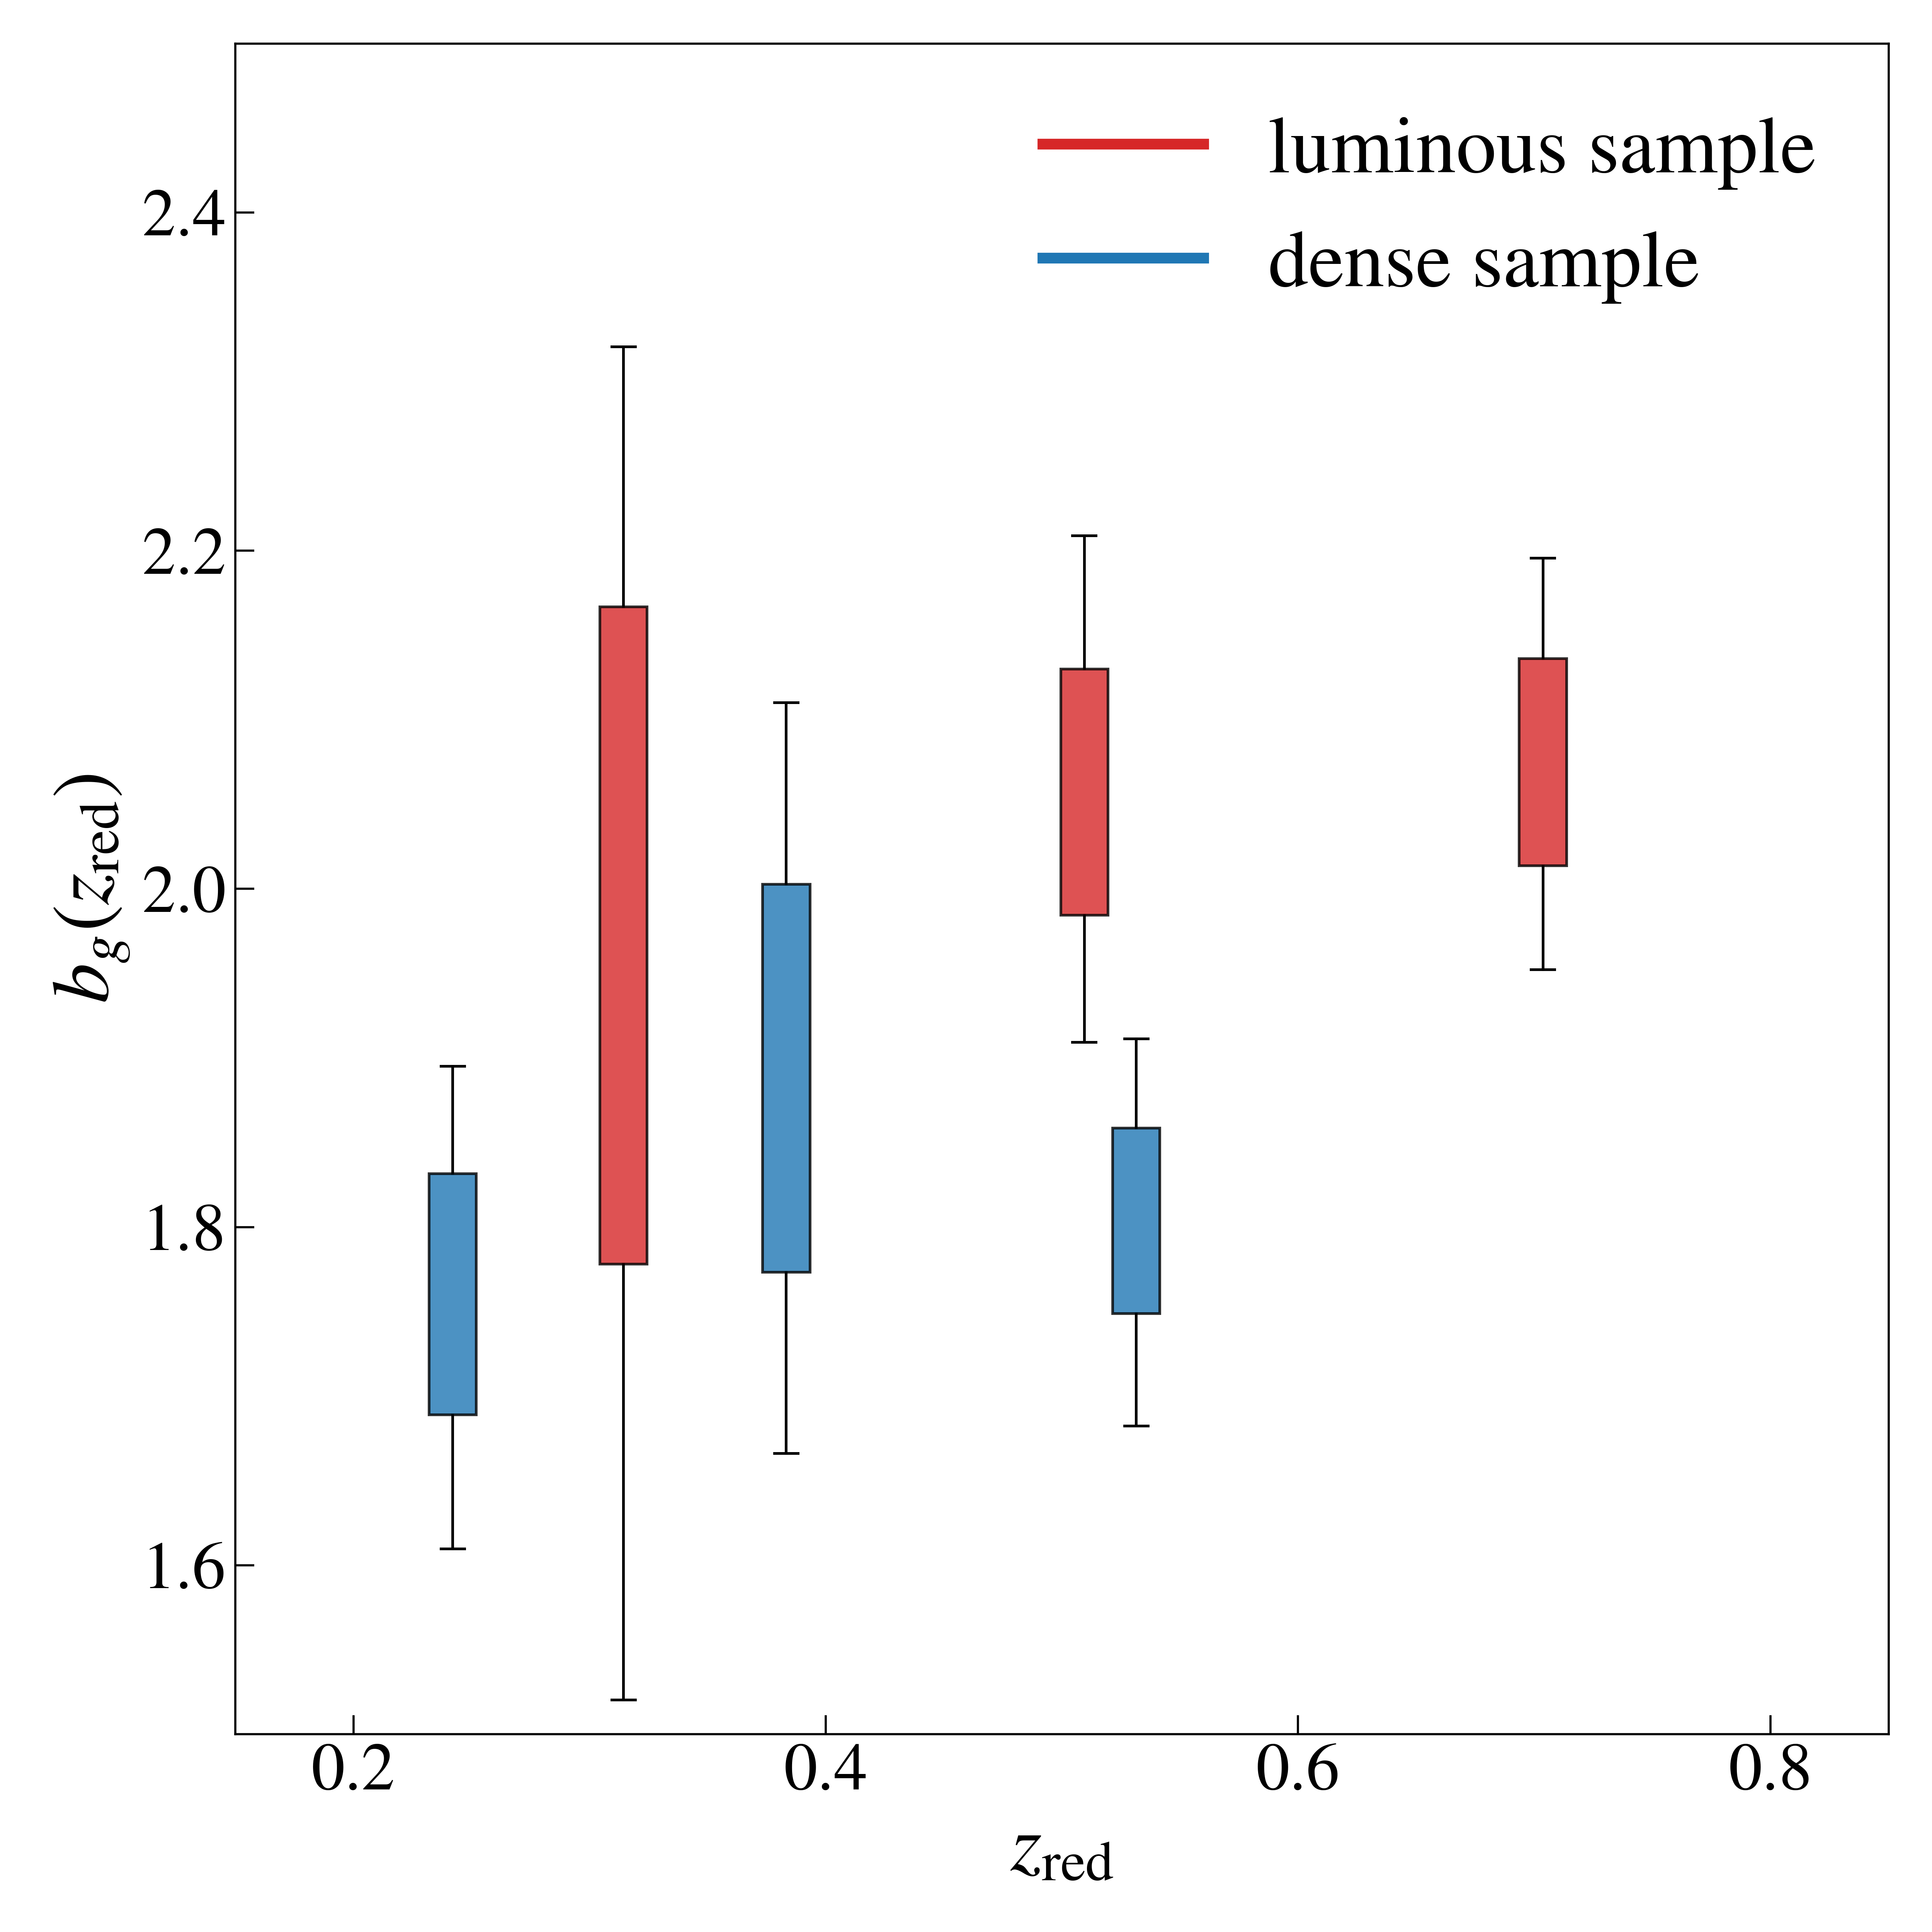
\includegraphics[width=\columnwidth]{figures_tmp/b_estimate_boxed.png}
\caption{ Redshift-dependence of the estimated linear galaxy bias shown for the dense sample (blue) and the luminous sample (red). The boxes mark the 68\% and the 95\% confidence intervals over the marginalized distribution over bias parameters. The solid (dashed) lines show the predictions of the passive evolution model of \citet{Fry1996} given the bias constraints in the three redshift bins (in the last redshift bin) for each galaxy sample.} 
\label{fig:b_estimate}
\end{figure}

%We tested the dependence of the inferred bias parameters on the brighness as well as the redshift of the subsamples. We defined two additional tomographic bins for galaxies in the luminous sample, with the edges $z_{\rm red} = [0.2,0.4, 0.6]$. 

\section{Summary}\label{sec:summary} 

In this work we have introduced selection and clustering measurements of the red-sequence galaxies in the fourth data release of the Kilo-Degree Survey. The data-driven colour-redshift relation of these galaxies, allows us to obtain precise and accurate estimates of their redshifts. We construct two samples, a bright one and a dense one, each with approximately constant comoving density.

We find that the near-infrared magnitudes derived from the VIKING imaging of the selected galaxies allow us to assess the purity of the sample. This purity assessment is done by comparing the colour distribution of the red-sequence candidates and that of high confidence stars in the fourth data release. The outcome of this procedure is the removal of the $\sim40\%$ of the candidates in the dense sample with $z_{\rm red}>0.6$ and $\sim5\%$ of the the candidates in the luminous sample in the same redshift range.

After taking into account the purity and completeness of the samples, we construct four redshift bins for our large-scale structure analysis with the first three bins based on the dense sample and the last bin based on the bright sample. 
In order to estimate the redshfit distributions as well as the uncertainty over the mean redshift of the distributions, we rely on four spectroscopic redshift surveys. Of these redshift surveys, three have overlap with the fourth data release, while GAMA-G10 only covers one of the KiDS calibration fields in the COSMOS region. In each tomographic bin, the individual redshift distributions of galaxies are well described by a Student-t distribution, parameters of which are estimated with the overlapping spectroscopic data sets. %\mb{[is it the case? I thought that the scaled errors are t-distributed and not the whole $dN/dz$?]}

In order to account for the survey systematics, we extend the works of \citet{bautista2018sdss} and \citet{icaza2020clustering} to allow for a more flexible relation between the systematic-induced variations of observed galaxy densities and the survey properties, while making use of heavy regularization to avoid overfitting. In comparison to \citet{ross2012clustering, crocce2019dark}, our adopted framework for removing the impact of survey properties does not make any assumption regarding the lack of correlation between the systematic parameters. Having validated our method for removing the effect of imaging systematics on the observed density variations, we apply the derived photometric weights to the measurement of the red-sequence galaxy clustering.

In order to avoid confirmation bias in our theoretical interpretation of the clustering measurements, we adopt a blinding method introduced by \citet{sellentin2019} in which the estimated inverse covariance matrix of the clustering measurements is perturbed. This perturbation manifest itself in shifting the posterior probability distributions over model parameters. 

We find that the estimated bias parameters of the galaxies in the $L>0.5L_{\star}$ sample are lower than those of $L>L_{\star}$ sample, consistent with the expectation that brighter galaxies reside in higher mass halos. The constraints on the photo-z shift parameters are consistent with zero and largely consistent with the adopted priors over these parameters. By comparing the redshift evolution of our bias constraints with the passive evolution model, we find that the bias evolution of galaxies in the $L>L_{\star}$ ($L>0.5L_{\star}$) sample is consistent (inconsistent) with the expectations of the model. 

The large-scale analysis of this study will be the cornerstone of our future 3$\times$2pt analysis for constraining the cosmological parameters with combination of the positions of red-sequence galaxies and cosmic shear signal of the background sources in the fourth data release of the Kilo-Degree Survey. The galaxy sample constructed in this work is also being used for constraining the intrinsic alignment of galaxies (Fortuna et al. in prep).


\section*{Acknowledgements}

MV and HHo acknowledge
support from Vici grant 639.043.512 from the Netherlands
Organization of Scientific Research (NWO).

GAMA is a joint European-Australasian project based
around a spectroscopic campaign using the Anglo Australian
Telescope. The GAMA input catalogue is based on data
taken from the Sloan Digital Sky Survey and the UKIRT
Infrared Deep Sky Survey. Complementary imaging of the
GAMA regions is being obtained by a number of independent survey programs including GALEX MIS, VST
KiDS, VISTA VIKING, WISE, Herschel-ATLAS, GMRT
and ASKAP providing UV to radio coverage. GAMA is
funded by the STFC (UK), the ARC (Australia), the AAO,
and the participating institutions. The GAMA website is
\hyperlink{www.gama-survey.org}{www.gama-survey.org}.

Funding for SDSS-III was provided by the Alfred P.
Sloan Foundation, the Participating Institutions, the National Science Foundation, and the U.S. Department of
Energy Office of Science. The SDSS-III website is \hyperlink{http:
//www.sdss3.org/}{http:
//www.sdss3.org/}. SDSS-III is managed by the Astrophysical Research Consortium for the Participating Institutions
of the SDSS-III Collaboration including the University of
Arizona, the Brazilian Participation Group, Brookhaven
National Laboratory, Carnegie Mellon University, University of Florida, the French Participation Group, the German Participation Group, Harvard University, the Instituto de Astrofisica de Canarias, the Michigan State/NotreDame/JINA Participation Group, Johns Hopkins University, Lawrence Berkeley National Laboratory, Max Planck
Institute for Astrophysics, Max Planck Institute for Extraterrestrial Physics, New Mexico State University, New
York University, Ohio State University, Pennsylvania State
University, University of Portsmouth, Princeton University,
the Spanish Participation Group, University of Tokyo, University of Utah, Vanderbilt University, University of Virginia, University of Washington, and Yale University.

This work has made use of \hyperlink{www.python.org}{python},
including the packages \hyperlink{www.numpy.org}{numpy}, \hyperlink{www.scipy.org}{scipy}, \hyperlink{https://pandas.pydata.org/}{pandas}, and \hyperlink{https://scikit-learn.org/}{scikit-learn}. 
Plots have been produced with \hyperlink{matplotlib.org}{matplotlib} and \hyperlink{https://seaborn.pydata.org/}{seaborn}.

This work has made use of \hyperlink{cosmohub.pic.es}{CosmoHub}.
CosmoHub has been developed by the Port dInformacio Cientifica (PIC), maintained through a collaboration of the Institut de Fisica d Altes Energies (IFAE) and the Centro de Investigaciones Energeticas, Medioambientales y Tecnologicas (CIEMAT) and the Institute of Space Sciences (CSIC \& IEEC), and was partially funded by the "Plan Estatal de Investigacion Cientifica y Tecnica y de Innovacion" program of the Spanish government.

%\begin{figure*}
 
% \begin{tabular}{cc}
%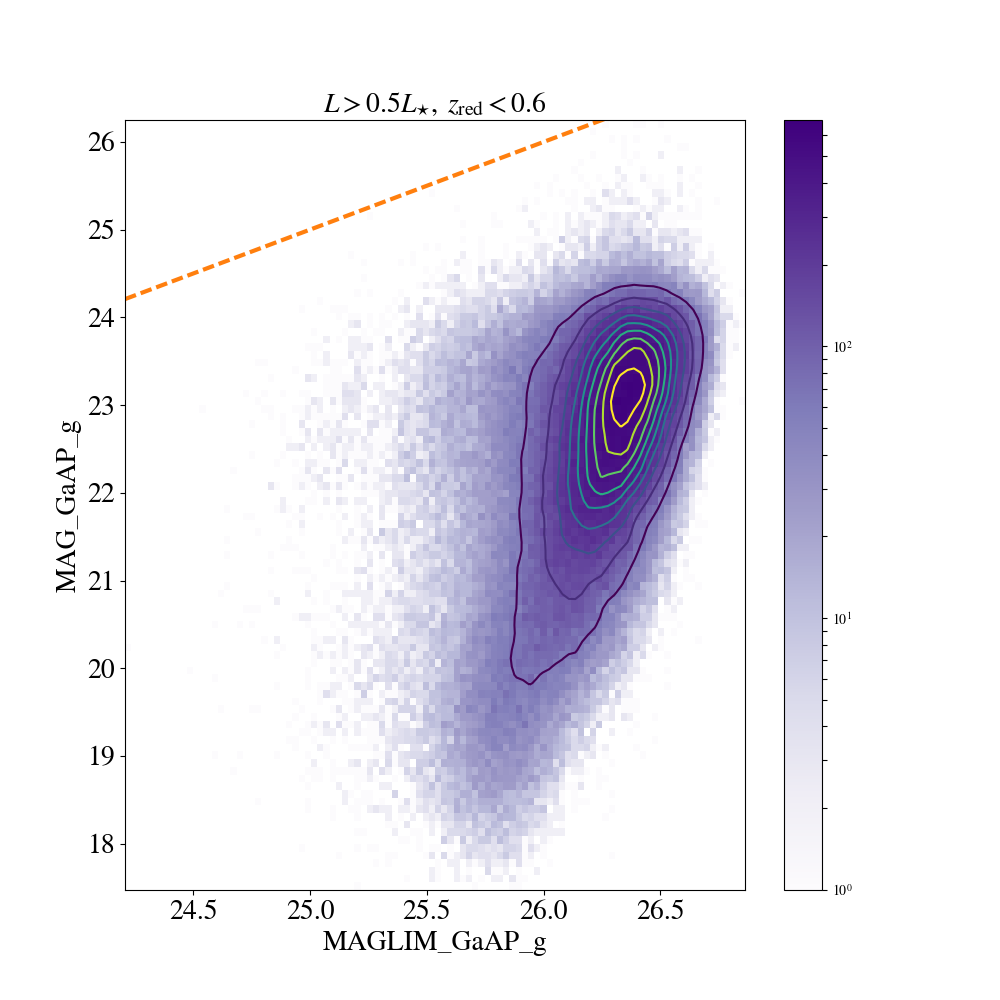
\includegraphics[width=0.5\textwidth]{figures_tmp/magg_lim_type_dense_zmax_0_6.png}
%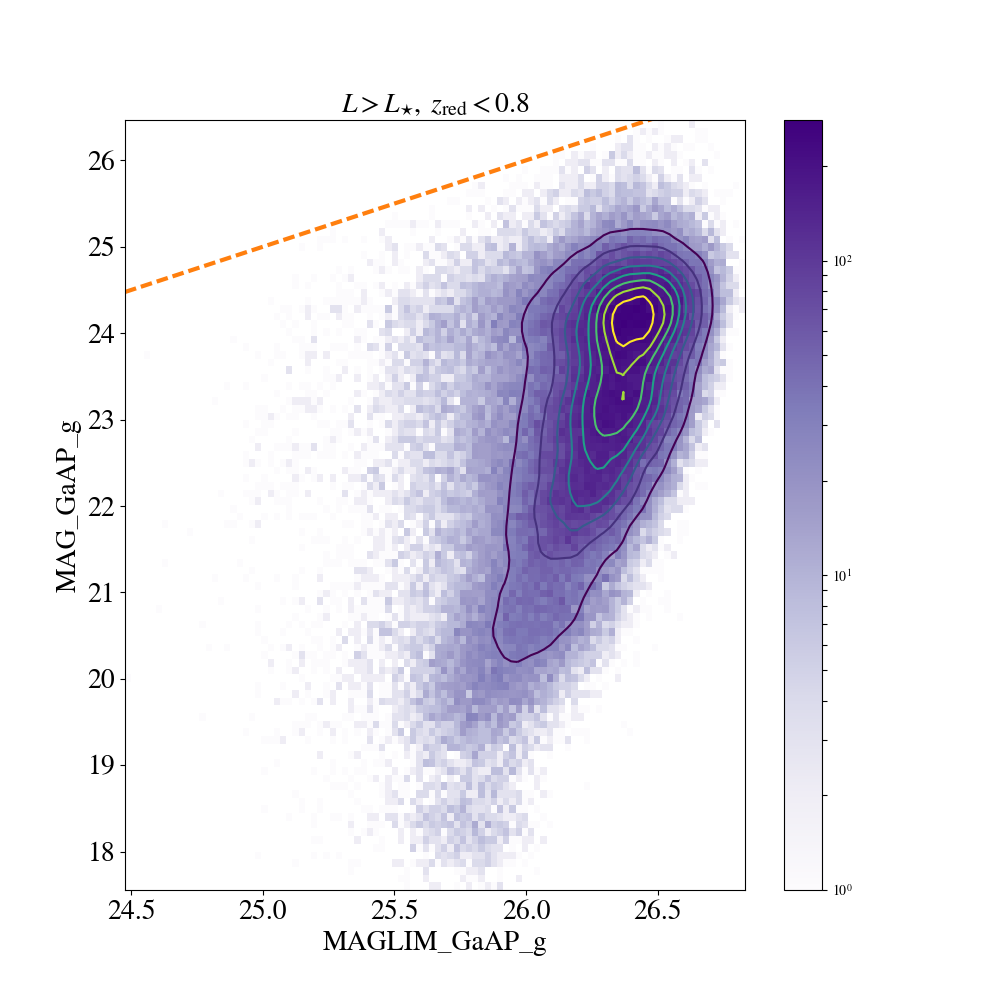
\includegraphics[width=0.5\textwidth]{figures_tmp/magg_lim_type_lum_zmax_0_8.png}
%\end{tabular}
%\caption{\label{fig:maglim_g} Demonstration of the distributions of the GaAP magnitudes and the limiting magnitudes in the $g$-band for the dense sample (left panel) and the luminous sample (right panel). In both figures the pixelised distributions and contours are colour-coded by the number counts. Note that the maximum redshifts of the two samples, $z_{\rm red}=0.6$ (dense) sample and $z_{\rm red}=0.8$ (luminous) sample are chosen such that the samples remain volume-limited and not limited by the varying depth of the survey (shown with the dashed orange line in both panels).} 
%\end{figure*}

%\begin{figure*}
 
% \begin{tabular}{cc}
%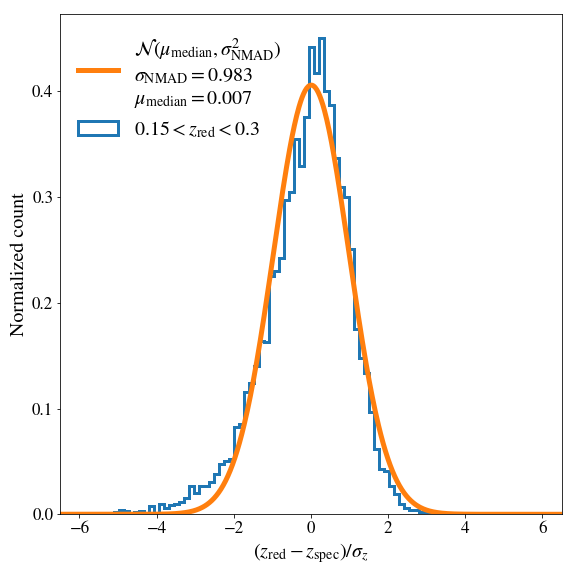
\includegraphics[width=0.5\textwidth]{figures_tmp/nz_normal_1.png}
%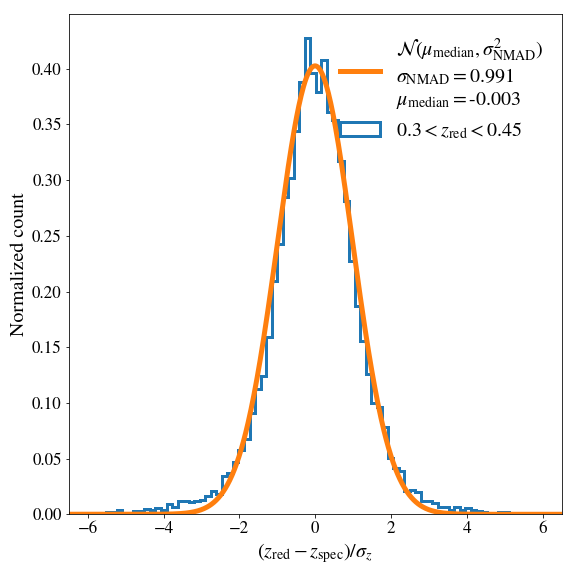
\includegraphics[width=0.5\textwidth]{figures_tmp/nz_normal_2.png}
%\end{tabular}

% \begin{tabular}{cc}
%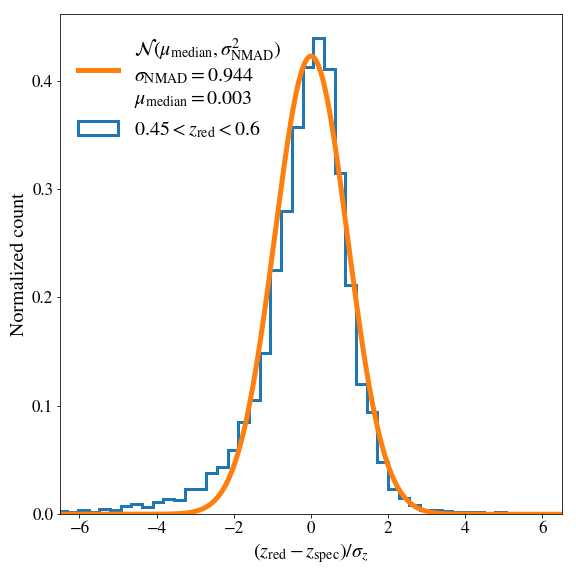
\includegraphics[width=0.5\textwidth]{figures_tmp/nz_normal_3.png}
%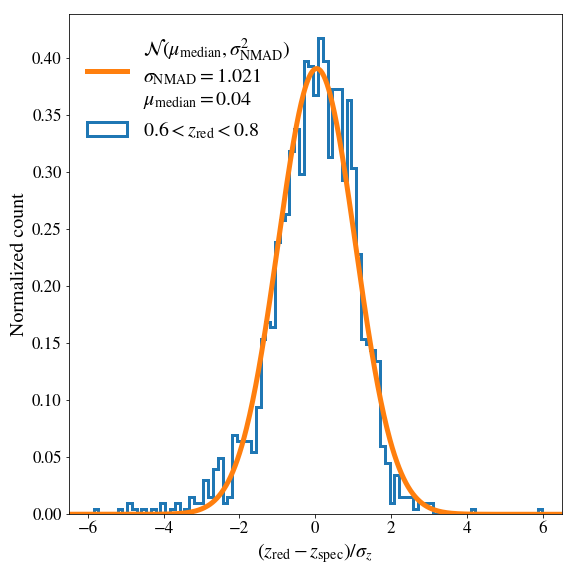
\includegraphics[width=0.5\textwidth]{figures_tmp/nz_normal_4.png}
%\end{tabular}
%\caption{\label{fig:pz} The Blue histogram shows the distribution of the offset between the red-sequence redshifts $z_{\rm red}$ and the spectroscopic redshifts $z_{\rm spec}$, weighted by their corresponding redshift uncertainties $\sigma_{z_{\rm red}}$. The orange solid line is a Gaussian distribution with zero mean and standard deviation of unity. This demonstrates that the a Gaussian distribution is a good description of the red-sequence redshift probability distribution functions of galaxies in the our sample of luminous red galaxies.} 
%\end{figure*}



%\begin{figure}
%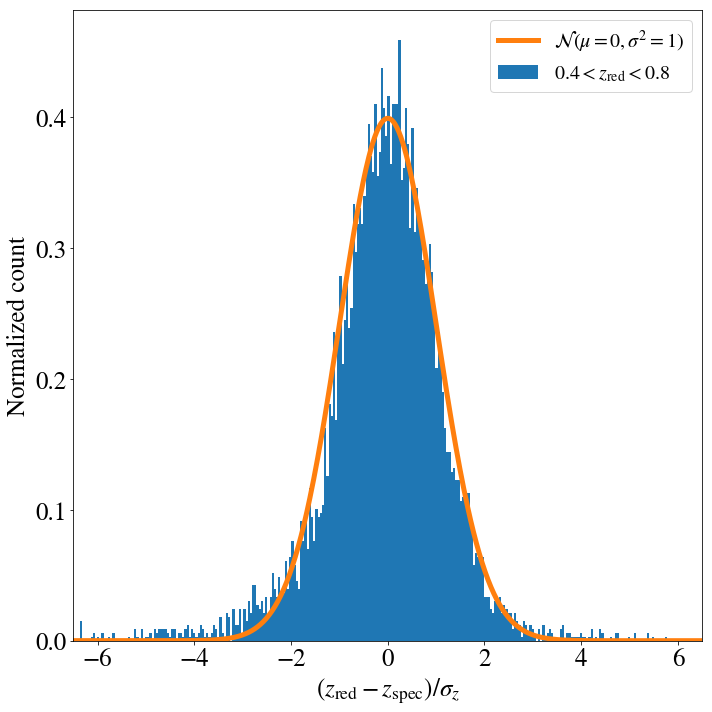
\includegraphics[width=\columnwidth]{figures_tmp/zerr_dist_2.png}
%\caption{\label{fig:pz} The Blue hisogram shows the distribution of the offset between the red-sequence redshifts $z_{\rm red}$ and the spectroscopic redshifts $z_{\rm spec}$, weighted by their corresponding redshift uncertainties $\sigma_{z_{\rm red}}$. The orange solid line is a Gaussian distribution with zero mean and standard deviation of unity. This demonstrates that the a Gaussian distribution is a good description of the red-sequence redshift probability distribution functions of galaxies in the our sample of luminous red galaxies.} 
%\end{figure}


%\begin{figure}
%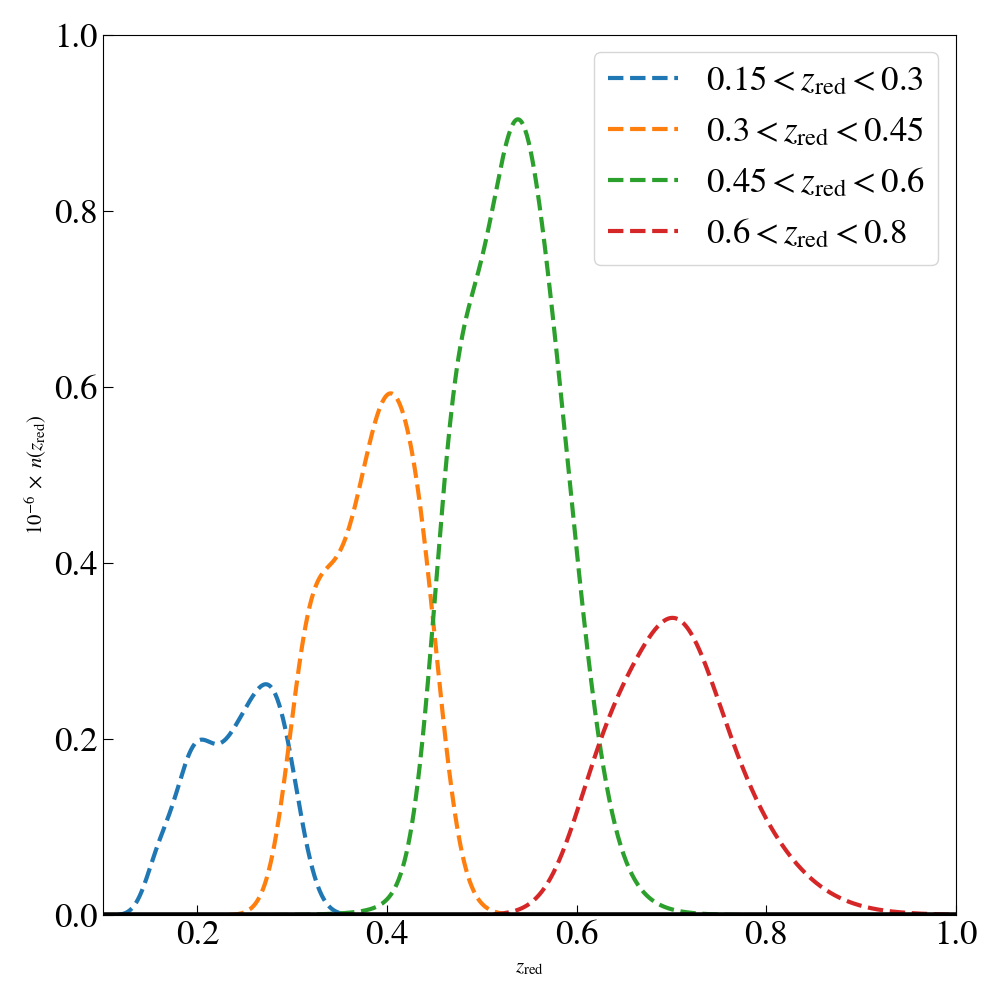
\includegraphics[width=\columnwidth]{figures_tmp/nofz.png}
%\caption{\label{fig:pz} Tomographic redshift distributions of our red galaxy sample in four bins: %$0.15<z_{\rm red}<0.3, \;0.3<z_{\rm red}<0.45, \;0.45<z_{\rm red}<0.6, \;0.6<z_{\rm red}<0.8$.
% The redshift distributions of the lenses are estimated directly from the the individual red-sequence %redshift estimates and their corresponding uncertainties.} 
%\end{figure}



%\begin{figure*}
%\begin{tabular}{cc}
%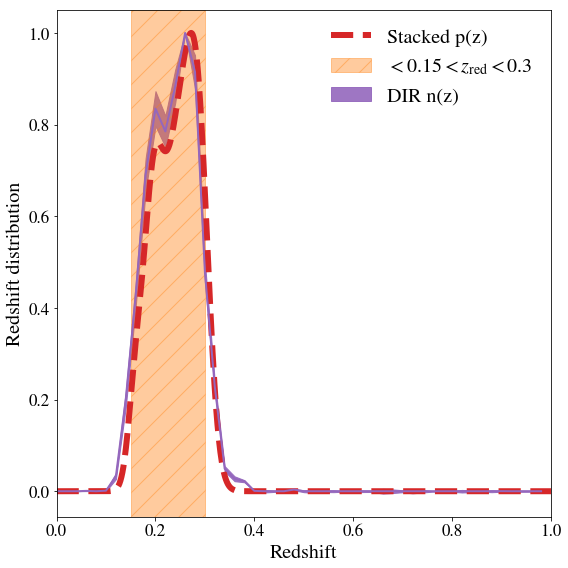
\includegraphics[width=\columnwidth]{figures_tmp/nz_comp_1.png}
%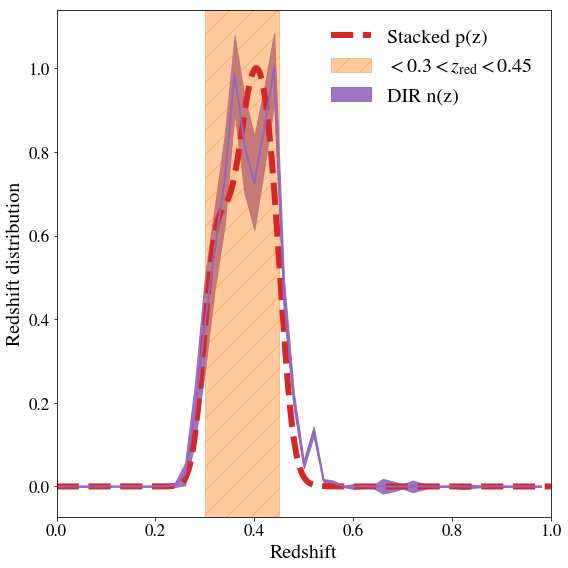
\includegraphics[width=\columnwidth]{figures_tmp/nz_comp_2.png}
%\end{tabular}
%\begin{tabular}{cc}
%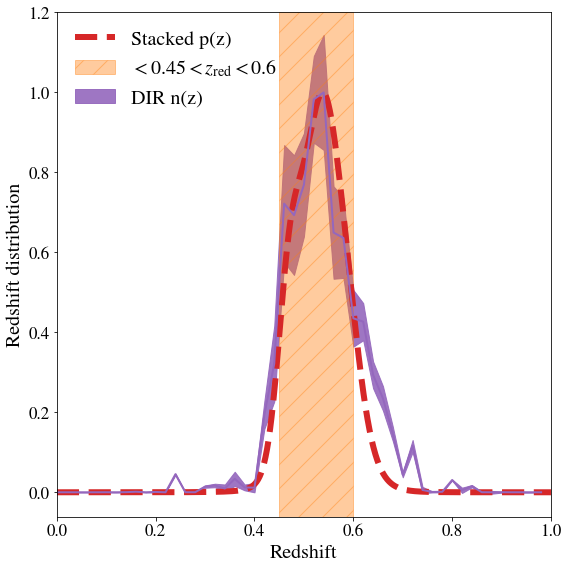
\includegraphics[width=\columnwidth]{figures_tmp/nz_comp_3.png}
%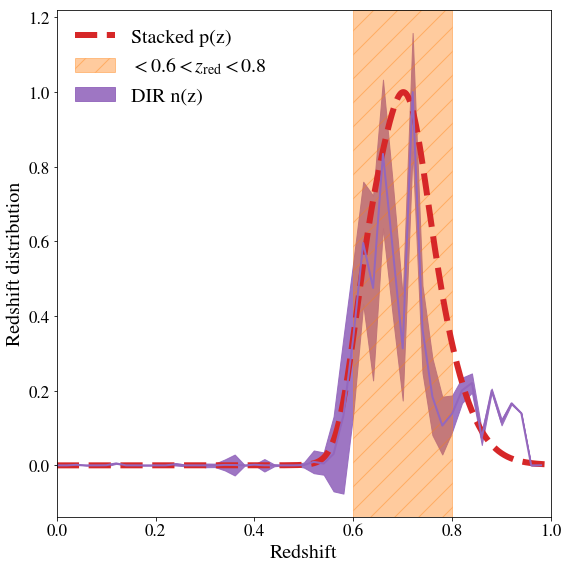
\includegraphics[width=\columnwidth]{figures_tmp/nz_comp_4.png}
%\end{tabular}
%
%\caption{\label{fig:pz2} Tomographic redshift distributions of our red galaxy sample in four bins: $0.15<z_{\rm red}<0.3, \;0.3<z_{\rm red}<0.45, \;0.45<z_{\rm red}<0.6, \;0.6<z_{\rm red}<0.8$.
% The redshift distributions are estimated from two methods: DIR redshift distributions are shown in blue and the stacked redshift probabilities are shown in orange.} 
%\end{figure*}





%%%%%%%%%%%%%%%%%%%%%%%%%%%%%%%%%%%%%%%%%%%%%%%%%%

%%%%%%%%%%%%%%%%%%%% REFERENCES %%%%%%%%%%%%%%%%%%
% BibTeX:

\bibliographystyle{mnras}
\bibliography{lrg_kids.bib}

%%%%%%%%%%%%%%%%%%%%%%%%%%%%%%%%%%%%%%%%%%%%%%%%%%

%%%%%%%%%%%%%%%%% APPENDICES %%%%%%%%%%%%%%%%%%%%%
%\clearpage

\appendix


\bsp	% typesetting comment
\label{lastpage}
\end{document}
